% xcolor cần tùy chọn table (cho \rowcolors) trước khi tikz nạp nó.
\PassOptionsToPackage{table}{xcolor}
\documentclass[a4paper, 12pt]{report}

% Tiếng Việt, mã hóa và ký hiệu toán.
\usepackage{vntex}
\usepackage[utf8]{inputenc}
\usepackage{amsmath,amssymb}

% Hình, vị trí float, caption căn giữa; thu hẹp khoảng trắng quanh hình/bảng.
\usepackage{graphicx}
\usepackage{float}
\usepackage{caption}
\captionsetup{justification=centering}
\setlength{\intextsep}{8pt plus 2pt minus 2pt}
\setlength{\textfloatsep}{10pt plus 2pt minus 2pt}
\setlength{\floatsep}{8pt plus 2pt minus 2pt}
\setlength{\abovecaptionskip}{5pt}
\setlength{\belowcaptionskip}{2pt}

% Lề trang (trái 3cm, phải 2cm, trên/dưới 2,5cm), giãn dòng 1,3, thụt đầu đoạn đầu tiên.
\usepackage[top=2.5cm,bottom=2.5cm,left=3cm,right=2cm,headheight=40pt,headsep=0.6cm,footskip=1.2cm,includehead]{geometry}
\usepackage{setspace}
\setstretch{1.3}
\usepackage{indentfirst}

% Bảng: cột co giãn, bảng nhiều trang, kẻ ngang, gộp dòng, màu nền; quy ước \tblsetup/\tblzebra/L{}.
\usepackage{array,tabularx,longtable,booktabs,multirow}
\usepackage{xcolor}
\definecolor{tblheadbg}{gray}{0.82}
\definecolor{tblaltbg}{gray}{0.95}
\newcolumntype{L}[1]{>{\raggedright\arraybackslash}p{#1}}
\newcommand{\tblsetup}{\small\renewcommand{\arraystretch}{1.25}\setlength{\tabcolsep}{5pt}}
\newcommand{\tblzebra}{\rowcolors{2}{}{tblaltbg}}

% Trang nằm ngang cho Gantt và bảng rộng.
\usepackage{pdflscape}

% Khối mã nguồn và thuật toán.
\usepackage{listings}
\definecolor{backcolour}{rgb}{0.95,0.95,0.92}
\lstset{frame=tb,
  backgroundcolor=\color{backcolour},
  basicstyle=\ttfamily\small,
  breaklines=true,
  captionpos=b,
  numbers=left,
  tabsize=2,
}
\usepackage[lined,boxed,commentsnumbered]{algorithm2e}

% Sơ đồ (activity network, PFD, PBS).
\usepackage{tikz}
\usetikzlibrary{arrows.meta,positioning,shapes,calc,backgrounds}

% Trích dẫn trong câu (\enquote); tài liệu tham khảo viết tay ở cuối, không cần biber.
\usepackage{csquotes}

% Header logo + tên trường/khoa, footer số trang; trang mở chương dùng chung kiểu.
\usepackage{fancyhdr}
\usepackage{lastpage}
\pagestyle{fancy}
\fancyhead{}
\fancyhead[L]{%
  \raisebox{-0.5\height}{
\includegraphics[height=8mm]{image/hcmut.png}}\hspace{2mm}%
  \parbox[c]{12cm}{\small\bfseries\setstretch{1}%
    Trường Đại học Bách Khoa -- ĐHQG TP.HCM\\
    Khoa Khoa học và Kỹ thuật Máy tính}}
\fancyfoot{}
\fancyfoot[R]{\small Trang \thepage}
\renewcommand{\headrulewidth}{0.3pt}
\renewcommand{\footrulewidth}{0.3pt}
\fancypagestyle{plain}{}

% Ghi chú việc cần điền: khung nền vàng nhạt, chữ nghiêng (khối trong đoạn, nội dòng trong ô bảng).
\definecolor{todobg}{RGB}{255,248,196}
\newcommand{\todo}[1]{%
  \ifvmode
    \par\noindent\colorbox{todobg}{\parbox{\dimexpr\linewidth-2\fboxsep\relax}{\itshape\small Cần điền: #1}}\par
  \else
    \colorbox{todobg}{\itshape\small #1}%
  \fi}

% Ghi chú rà soát bản nháp: cam = cần kiểm tra lại (đã có nội dung nhưng chưa chắc/nháp AI); đỏ hồng = cần nhóm chốt.
\definecolor{checkbg}{RGB}{255,213,153}
\definecolor{decidebg}{RGB}{255,189,196}
\newcommand{\kiemtra}[1]{%
  \ifvmode
    \par\noindent\colorbox{checkbg}{\parbox{\dimexpr\linewidth-2\fboxsep\relax}{\small\textbf{Cần kiểm tra lại:} #1}}\par
  \else
    \colorbox{checkbg}{\small #1}%
  \fi}
\newcommand{\chot}[1]{%
  \ifvmode
    \par\noindent\colorbox{decidebg}{\parbox{\dimexpr\linewidth-2\fboxsep\relax}{\small\textbf{Cần chốt:} #1}}\par
  \else
    \colorbox{decidebg}{\small\textbf{#1}}%
  \fi}

% Đánh số tới subsubsection, mục lục tới section.
\setcounter{secnumdepth}{3}
\setcounter{tocdepth}{1}

% Việt hóa tên chương, phụ lục, hình, bảng, mục lục, danh mục.
\AtBeginDocument{%
  \renewcommand*\chaptername{Chương}%
  \renewcommand*\appendixname{Phụ lục}%
  \renewcommand*\figurename{Hình}%
  \renewcommand*\tablename{Bảng}%
  \renewcommand*\contentsname{Mục lục}%
  \renewcommand*\listfigurename{Danh mục hình}%
  \renewcommand*\listtablename{Danh mục bảng}%
}

% Liên kết nội bộ; nạp gần cuối để không xung đột gói khác.
\usepackage{hyperref}
\hypersetup{urlcolor=blue,linkcolor=black,citecolor=black,colorlinks=true}
% Cho URL dài (Drive, Sheet) xuống dòng giữa chữ và số.
\expandafter\def\expandafter\UrlBreaks\expandafter{\UrlBreaks\do\a\do\b\do\c\do\d\do\e\do\f\do\g\do\h\do\i\do\j\do\k\do\l\do\m\do\n\do\o\do\p\do\q\do\r\do\s\do\t\do\u\do\v\do\w\do\x\do\y\do\z\do\A\do\B\do\C\do\D\do\E\do\F\do\G\do\H\do\I\do\J\do\K\do\L\do\M\do\N\do\O\do\P\do\Q\do\R\do\S\do\T\do\U\do\V\do\W\do\X\do\Y\do\Z\do0\do1\do2\do3\do4\do5\do6\do7\do8\do9}
\begin{document}

% ===================== TRANG BÌA =====================
\begin{titlepage}
\begin{center}
ĐẠI HỌC QUỐC GIA THÀNH PHỐ HỒ CHÍ MINH \\
TRƯỜNG ĐẠI HỌC BÁCH KHOA \\
KHOA KHOA HỌC VÀ KỸ THUẬT MÁY TÍNH

\vspace{1cm}

\includegraphics[width=3cm]{image/hcmut.png}
\vspace{1cm}

\begin{tabular}{c}
\textbf{\normalsize QUẢN LÝ DỰ ÁN PHẦN MỀM (CO3011)} \\
\textbf{\normalsize Lớp L01 -- Nhóm 9} \\[4pt]
\hline \\
\textbf{\Large HỆ THỐNG ĐĂNG KÝ VÀ QUẢN LÝ SỰ KIỆN} \\[4pt]
\textit{\large University Event Registration System} \\[8pt]
\hline
\end{tabular}

\vspace{0.6cm}
Giảng viên: Nguyễn Minh Tâm

\vspace{0.7cm}
\begin{tabular}{|c|l|c|l|}
\hline
\textbf{STT} & \textbf{Họ tên} & \textbf{MSSV} & \textbf{Vai trò} \\
\hline
1 & Nguyễn Đức Nghĩa & 2312266 & Project Manager \\
\hline
2 & Ngô Thanh Hùng & 2311289 & BA / QA \\
\hline
3 & Phan Huy Quang Minh & 2312105 & Tech Lead, Backend \\
\hline
4 & Nguyễn Đắc Nghĩa & 2312265 & Frontend \\
\hline
5 & Hà Cao Đức Minh & 2312059 & Fullstack, DevOps \\
\hline
\end{tabular}

\vfill
Thành phố Hồ Chí Minh, tháng 12 năm 2026
\end{center}
\end{titlepage}

% ===================== MỤC LỤC, DANH MỤC =====================
\pagenumbering{roman}
\tableofcontents
\cleardoublepage\phantomsection
\addcontentsline{toc}{chapter}{Danh mục hình}
\listoffigures
\cleardoublepage\phantomsection
\addcontentsline{toc}{chapter}{Danh mục bảng}
\listoftables
\clearpage
\noindent\textbf{Chú giải ghi chú trong bản nháp} (xóa trang này và mọi ghi chú màu trước khi nộp):\par\medskip
\noindent\colorbox{todobg}{\parbox{\dimexpr\linewidth-2\fboxsep\relax}{\itshape \small Vàng -- Cần điền: chưa có dữ liệu, phải bổ sung.}}\par\smallskip
\noindent\colorbox{checkbg}{\parbox{\dimexpr\linewidth-2\fboxsep\relax}{\small Cam -- Cần kiểm tra lại: đã có nội dung nhưng là bản nháp AI, số chưa khớp hoặc cần người phụ trách xác nhận.}}\par\smallskip
\noindent\colorbox{decidebg}{\parbox{\dimexpr\linewidth-2\fboxsep\relax}{\small Đỏ hồng -- Cần chốt: nhóm phải ra quyết định trước khi hoàn thiện mục này.}}\par\smallskip
\clearpage

% ===================== NỘI DUNG CHÍNH =====================
% Phần nội dung đánh số lại từ 1; chân trang hiển thị "Trang x/tổng".
\pagenumbering{arabic}
\fancyfoot[R]{\small Trang \thepage/\pageref{LastPage}}
\chapter{Khởi động - xác định dự án (Task 1)}
\label{chap:task1}

\section{Tham vấn client và Client Interaction Log}
\label{sec:1-1}

Thầy Nguyễn Minh Tâm đóng vai client của dự án (P01). Các vòng trao đổi đến thời điểm hiện tại:

\begingroup\tblsetup\tblzebra
\begin{longtable}{L{1.6cm}L{3.2cm}L{3.2cm}L{6.0cm}}
\caption{Các vòng trao đổi với client}\label{tab:client-rounds}\\
\toprule
\rowcolor{tblheadbg}\textbf{Vòng} & \textbf{Gửi} & \textbf{Client trả lời} & \textbf{Nội dung} \\
\midrule
\endfirsthead
\toprule
\rowcolor{tblheadbg}\textbf{Vòng} & \textbf{Gửi} & \textbf{Client trả lời} & \textbf{Nội dung} \\
\midrule
\endhead
\bottomrule
\endlastfoot
P01 & 23/09/2026 20:25, Nguyễn Đức Nghĩa & 24/09/2026 07:48 & Vai trò client \\
Q01--Q09 & 02/10/2026 15:17, Nguyễn Đức Nghĩa & 02/10/2026 19:48 & Nghiệm thu, điểm danh, số chỗ/waitlist, tổ chức sự kiện, đăng nhập, báo cáo, quy mô, ràng buộc, hiện trạng \\
Q10--Q17, Q19--Q20 & 08/10/2026 16:39, Nguyễn Đức Nghĩa & 08/10/2026 19:58 & Xác nhận scope và MoE; role duyệt, hạn hủy, waitlist, đăng ký trùng, sửa/hủy sự kiện, quyền xem dữ liệu; milestone môn học; change event \\
Q21--Q22 (A58) & 23/10/2026 15:10, Nguyễn Đức Nghĩa & 25/10/2026 07:32 & Phạm vi demo tại Progress Check 09/11; kênh thông báo tối thiểu \\
\end{longtable}
\endgroup

Câu hỏi vòng 1 được chia theo 3 mức ưu tiên dựa trên tác động: mức 1 tác động lớn tới scope và rủi ro (Q08, Q03, Q04); mức 2 tác động tới luồng dữ liệu và thiết kế (Q01, Q02, Q05); mức 3 phục vụ giả định và đo lường (Q06, Q09, Q07). Mỗi câu hỏi mức 1--2 có kèm phân tích tác động và câu hỏi follow-up chuẩn bị trước. Nội dung đầy đủ của từng lần trao đổi ở Phụ lục~\ref{app:client-log}.

Vòng 2 (phản hồi ngày 08/10) xác nhận phạm vi và mục tiêu (Q10, Q11), chốt các quy tắc nghiệp vụ (Q12--Q15, Q19, Q20) và làm rõ lịch môn học (Q16, Q17). Các thay đổi chính đối với dự án:
\begin{itemize}
  \item Admin hệ thống thực hiện việc duyệt sự kiện, không tách thêm role riêng; Organizer không được tự duyệt sự kiện của mình (Q12).
  \item Hạn hủy đăng ký cố định 24 giờ trước giờ bắt đầu sự kiện (Q13).
  \item Organizer được sửa hoặc hủy sự kiện đã công bố; hệ thống phải thông báo người đã đăng ký khi đổi thời gian hoặc địa điểm (Q19). Đây là yêu cầu mới so với vòng 1.
  \item Môn học không có Milestone 2 và 3, chỉ có một lần Progress Check theo kế hoạch (Q16).
  \item Change event không báo trước nội dung; nhóm xem là rủi ro và dành contingency, không tạo trước activity riêng (Q17).
\end{itemize}

Vòng 2 gửi lúc 16:39 và được thầy trả lời lúc 19:58 cùng ngày 08/10; ảnh bằng chứng \texttt{Q10-Q20-2026-10-08-email-tra-loi.png} (P06) lưu trong thư mục minh chứng trên Drive của nhóm (Phụ lục~\ref{app:repository}).

\kiemtra{Cột \enquote{Tác động} ở Phụ lục~\ref{app:client-log} cho vòng 2 là đề xuất của AI, TV1 rà lại.}

Vòng 3 (A58) được gửi khi lịch A21 cho thấy đến 09/11 chưa có QR check-in; thầy trả lời sáng 25/10, trước họp A23. Thầy đồng ý phạm vi nhóm đề xuất (Q21): tại Progress Check chưa bắt buộc hoàn thiện toàn bộ workflow, gồm QR check-in và báo cáo/Excel/CSV, nhưng chức năng đã hoàn thành phải có bản demo chạy được, không chỉ trình bày giao diện hoặc mô tả thiết kế; chức năng đang phát triển phải thể hiện rõ tiến độ và kế hoạch hoàn thành. Thầy đồng ý thông báo trong ứng dụng là mức bắt buộc, email là mức Should (Q22). Nhóm sửa tiêu chí CP4 (mục~\ref{sec:2-5}) theo Q21, không đổi thứ tự công việc.

\kiemtra{Ảnh chụp email trả lời Q21, Q22 (TV1 cung cấp 27/10) cần lưu lên Drive làm bằng chứng (P06), đề xuất tên \texttt{Q21-Q22-2026-10-25-email-tra-loi.png}.}

\todo{Bổ sung: bằng chứng client đã làm thay đổi quyết định (scope, estimate, risk) cụ thể ra sao ở Baseline V1.0.}

\section{Bối cảnh, giả định và ràng buộc}
\label{sec:1-2}

\subsection*{Bối cảnh tổ chức}
Trường thường xuyên tổ chức seminar, workshop và hoạt động cho sinh viên. Sự kiện có thể do Khoa, CLB/Đội/Nhóm và các đơn vị/phòng ban của trường tổ chức. Các đơn vị này có thể tạo sự kiện, nhưng sự kiện phải được một vai trò có thẩm quyền (authorized role) phê duyệt trước khi công bố (Q01). Sinh viên là nhóm người tham gia chính; Organizer (Ban tổ chức) và Admin (quản trị viên hệ thống, đồng thời duyệt sự kiện) quản lý thông tin sự kiện và dữ liệu tham dự.

Quy trình hiện tại dùng form/bảng tính và có một số bước tổng hợp thủ công (Q07). Đây là planning assumption, không phải số liệu đo thực tế của nhà trường.

\subsection*{Vấn đề và cơ hội}
Thông tin sự kiện, đăng ký tham dự và điểm danh đang được quản lý bằng nhiều công cụ khác nhau. Workflow phân mảnh có thể buộc Ban tổ chức đối soát thủ công dữ liệu đăng ký, sức chứa, danh sách chờ (waitlist), điểm danh và báo cáo sau sự kiện. Cơ hội của dự án là xây dựng một hệ thống web responsive duy nhất, duy trì trạng thái người tham gia nhất quán từ khi sự kiện được công bố, qua đăng ký, điểm danh, đến báo cáo.

\subsection*{Sản phẩm đề xuất và hướng đã xác nhận}
\begin{itemize}
  \item Ứng dụng web responsive; không bắt buộc ứng dụng mobile native (Q09).
  \item Đăng nhập mô phỏng tài khoản trường bằng tài khoản mẫu có email trường (ASM-06); không tích hợp SSO thật (Q02).
  \item Phân quyền theo vai trò (RBAC) cho Student, Organizer và Admin; sự kiện phải được Admin duyệt trước khi công bố, Organizer không được tự duyệt sự kiện của mình (Q01, Q09, Q12). Organizer chỉ xem dữ liệu sự kiện do mình quản lý; Admin xem dữ liệu các đơn vị được giao duyệt; sinh viên chỉ xem đăng ký của chính mình (Q20).
  \item Quản lý số chỗ, đăng ký/hủy, waitlist; khi có chỗ trống tự động chuyển người đứng đầu waitlist sang danh sách đăng ký và thông báo cho người đó (Q04). Hủy được đến 24 giờ trước giờ bắt đầu (Q13); thông báo thất bại vẫn tính là đã đăng ký, không có trạng thái chờ xác nhận (Q14); sinh viên đã hủy được đăng ký lại, vào cuối waitlist nếu sự kiện đã đầy (Q15).
  \item Organizer được sửa hoặc hủy sự kiện đã công bố; đổi thời gian hoặc địa điểm thì thông báo người đã đăng ký; hủy sự kiện thì hủy các đăng ký, đóng waitlist và thông báo (Q19).
  \item Điểm danh bằng QR, có phương án dự phòng nhập mã hoặc xác nhận thủ công; không yêu cầu check-out (Q03).
  \item Báo cáo gồm danh sách đăng ký, danh sách điểm danh, thống kê số lượng tham gia, xuất Excel/CSV; tích hợp trực tiếp với hệ thống điểm rèn luyện nằm ngoài scope (Q05).
  \item Nhắc lịch/thông báo chung là chức năng bổ trợ; client ưu tiên core workflow hơn (Q08).
\end{itemize}

\subsection*{Giả định}
\begingroup\tblsetup\tblzebra
\begin{longtable}{L{1.5cm}L{6.5cm}L{1.5cm}L{3.5cm}}
\caption{Các giả định của dự án}\label{tab:assumptions}\\
\toprule
\rowcolor{tblheadbg}\textbf{Mã} & \textbf{Nội dung} & \textbf{Cơ sở} & \textbf{Trạng thái} \\
\midrule
\endfirsthead
\toprule
\rowcolor{tblheadbg}\textbf{Mã} & \textbf{Nội dung} & \textbf{Cơ sở} & \textbf{Trạng thái} \\
\midrule
\endhead
\bottomrule
\endlastfoot
ASM-01 & Quy trình hiện tại dùng form/bảng tính, có một số bước tổng hợp thủ công. & Q07 & Client cho phép giả định \\
ASM-02 & Không có số liệu sử dụng thực tế (Q06). Nhóm giả định để thiết kế và kiểm thử: khoảng 20 sự kiện mỗi tháng trên toàn hệ thống; trung bình 100 và tối đa 500 người đăng ký mỗi sự kiện; tối đa 50 lượt check-in đồng thời; tối đa 100 lượt đăng ký đồng thời khi mở đăng ký. & Q06 & Giả định của nhóm; client cho phép \\
ASM-03 & Hạn chót hủy đăng ký: mốc cố định 24 giờ trước giờ bắt đầu sự kiện, áp dụng toàn hệ thống; sau mốc này sinh viên liên hệ Organizer. & Q04, Q13 & Client đồng ý (08/10) \\
ASM-04 & Admin hệ thống thực hiện việc duyệt, không tách role riêng; Organizer không tự duyệt sự kiện của mình. Mô hình: Student / Organizer / Admin. & Q01, Q12 & Client đồng ý nguyên tắc (08/10) \\
ASM-05 & Nếu cần hosting, nhóm dùng gói miễn phí hoặc môi trường tương đương vì client không đặt ràng buộc hosting. & Q09 & Giả định của nhóm; client không ràng buộc \\
ASM-06 & Tài khoản trường được mô phỏng bằng tài khoản mẫu có email trường (dạng \texttt{mã@hcmut.edu.vn}) và mật khẩu cục bộ, đủ ba vai trò Student, Organizer, Admin; không kết nối hệ thống của trường. & Q02 & Giả định của nhóm; client cho phép \\
ASM-07 & Mốc hiện trạng để so sánh MoE: điểm danh thủ công khoảng 15 giây mỗi người; tổng hợp sau sự kiện khoảng 20 phút mỗi sự kiện (O2, O3). Đây là số do nhóm đặt, không phải số đo thực. & Q07 & Giả định của nhóm; client cho phép \\
\end{longtable}
\endgroup

\kiemtra{Giá trị của ASM-02, ASM-06, ASM-07 do PM chốt ngày 12/10 dựa trên đề xuất của AI (đã ghi AI Log) và được ghi là giả định của nhóm vì client cho phép (Q02, Q06, Q07). Nhóm rà lại tính hợp lý và độ khớp với bộ kiểm thử 500 lượt đăng ký ở O3; giả định phải được dùng nhất quán ở Product Description, test plan và risk register.}

\subsection*{Ràng buộc}
\begin{itemize}
  \item \textbf{Lịch:} Milestone~1 trình bày ngày 05/10/2026; CP1 ngày 04/10/2026. Task~2 hoàn thành sau M1 và trước khi chốt Baseline V1.0. Theo thầy (08/10, Q16) môn học không có Milestone~2 và 3; chỉ có một lần Progress Check theo kế hoạch (09/11) và demo, viva ngày 07/12.
  \item \textbf{Nhân lực:} nhóm 5 sinh viên; công việc quản lý dự án và hiện thực dùng chung nguồn lực giới hạn.
  \item \textbf{Dữ liệu và quyền riêng tư:} cần phân quyền cơ bản và bảo vệ thông tin cá nhân của sinh viên (Q09).
  \item \textbf{Nền tảng:} web responsive là đủ; không yêu cầu mobile native (Q09).
  \item \textbf{Hosting:} client không áp đặt; lựa chọn triển khai là quyết định kỹ thuật của nhóm (Q09).
  \item \textbf{Bằng chứng:} Client Interaction Log phải lưu trao đổi và mốc thời gian thực tế; không cần biên bản có chữ ký riêng (P06).
\end{itemize}
\begin{itemize}
  \item \textbf{Công cụ:} GitHub, Jira và Google Sheet (mục~\ref{sec:1-7}); CI/CD do repo code đảm nhiệm.
  \item \textbf{Ngân sách:} không có ngân sách bằng tiền; vận hành dùng gói miễn phí (ASM-05).
\end{itemize}
Stack kỹ thuật được nhóm chốt tại họp ngày 18/10: React cho giao diện, Go cho API, PostgreSQL cho cơ sở dữ liệu. Trong nhóm đã có thành viên từng học và làm dự án với Go.

\kiemtra{Bổ sung kỹ năng của từng thành viên với React, Go, PostgreSQL (chưa dùng, đã học, đã làm dự án) nếu cần cho phân công và rủi ro.}

\section{Business case và quyết định go/no-go}
\label{sec:1-3}
\subsection*{Lợi ích kỳ vọng}
Hệ thống thay thế quy trình form/bảng tính và tổng hợp thủ công hiện tại (Q07, client cho phép giả định), giảm sai sót đối soát và tăng tốc điểm danh bằng QR. Mức cải thiện được đo bằng các MoE O1--O4 ở Bảng~\ref{tab:objectives}; mốc hiện trạng là planning assumption (mục~\ref{sec:1-2}).

\subsection*{Chi phí và bất lợi}
\begin{itemize}
  \item Công sức của 5 sinh viên trong thời gian môn học; effort chính thức được xác định ở Task~2 (A18), trước khi chốt Baseline V1.0; chi phí nhân công tính bằng giờ người, không quy đổi sang VND.
  \item Chi phí vận hành bằng tiền: 0 VND theo giả định dùng free-tier hosting (ASM-05, Q09).
  \item Các đơn vị (Khoa, CLB/Đội/Nhóm) cần thời gian làm quen hệ thống; xử lý bằng tài liệu hướng dẫn giao diện. Nhóm đánh giá mức rủi ro thấp.
  \item Phạm vi giới hạn: không SSO thật, không tích hợp hệ thống điểm rèn luyện.
\end{itemize}

\subsection*{Phương án thay thế}
Giữ form/bảng tính như hiện trạng (Q07): không tốn công xây dựng nhưng vẫn phải đối soát thủ công. Việc dùng công cụ có sẵn chưa được nhóm khảo sát.

\subsection*{Tiêu chí và kết luận go/no-go}
Chưa áp dụng đánh giá tài chính (NPV, ROI) vì không có số liệu thực tế. Khuyến nghị: \textbf{GO}, vì chi phí vận hành bằng tiền bằng 0 (theo giả định free-tier) và hệ thống giải quyết đúng điểm đau thủ công hiện tại. Quyết định được đánh giá lại khi chốt Baseline V1.0, vì ước lượng effort chính thức chỉ có ở Task~2.

\textbf{Go nếu:}
\begin{itemize}
  \item Workflow cốt lõi rõ và được client xác nhận (Q08).
  \item Chi phí vận hành bằng tiền bằng 0 theo giả định free-tier (ASM-05).
  \item Không phụ thuộc hệ thống ngoài: không SSO thật, không tích hợp điểm rèn luyện (Q02, Q05).
\end{itemize}

\textbf{No-go nếu} (xét lại ở Baseline V1.0):
\begin{itemize}
  \item Client đổi hướng ưu tiên lớn hoặc yêu cầu tích hợp hệ thống ngoài.
  \item Effort ước lượng ở Task~2 vượt khả năng của 5 sinh viên, hoặc lịch vượt Progress Check 09/11 mà không thu hồi được.
\end{itemize}
\textbf{Xử lý khi no-go:} họp với client để thu hẹp scope, bỏ nhóm Could rồi Should (Bảng~\ref{tab:moscow}) trước, không bỏ core workflow.

Kết luận GO và các tiêu chí go/no-go ở trên đã được TV4 (phụ trách A06) xác nhận trong báo cáo Milestone~1.


Hướng xử lý (PM chốt 13/10): nếu ước lượng hoặc lịch của Task~2 vượt khả năng của 5 sinh viên hoặc vượt Progress Check 09/11 thì thu hẹp phạm vi theo thứ tự Could rồi Should, không bỏ core workflow. Bản đề xuất sơ bộ (nháp AI) cho thấy lịch có thể vượt, nên kết luận GO hiện là khuyến nghị có điều kiện.

\section{Phạm vi, loại trừ, mục tiêu và thước đo hiệu quả (MoE)}
\label{sec:1-4}

\subsection*{Phạm vi}
Dự án cung cấp hệ thống đăng ký và quản lý sự kiện dạng web responsive, bao phủ các workflow cốt lõi mà client ưu tiên nghiệm thu theo thứ tự (Q08):
\begin{enumerate}
  \item Tạo và quản lý sự kiện; sự kiện phải được Admin duyệt trước khi công bố, Organizer không được tự duyệt sự kiện của mình (Q01, Q12).
  \item Sinh viên đăng ký và hủy đăng ký; hủy được đến 24 giờ trước giờ bắt đầu (Q13); mỗi sinh viên chỉ có một đăng ký còn hiệu lực cho một sự kiện, hủy rồi được đăng ký lại (Q15).
  \item Quản lý số lượng và danh sách chờ: sự kiện có giới hạn số chỗ; khi có chỗ trống, hệ thống tự động chuyển người đầu waitlist sang danh sách đăng ký và gửi thông báo, không cần ban tổ chức duyệt lại (Q04); thông báo thất bại vẫn tính là đã đăng ký (Q14).
  \item Điểm danh bằng QR, có phương án dự phòng nhập mã hoặc xác nhận thủ công (Q03).
  \item Xem kết quả và báo cáo: danh sách đăng ký, danh sách điểm danh, thống kê số người tham gia; có thể xuất Excel/CSV (Q05).
\end{enumerate}
Thông báo và nhắc lịch là chức năng bổ trợ, ưu tiên thấp hơn các workflow trên (Q08). Ngoài ra, theo phản hồi 08/10 (Q19), Organizer được sửa hoặc hủy sự kiện đã công bố; khi đó hệ thống thông báo người đã đăng ký (đổi thời gian hoặc địa điểm) hoặc hủy đăng ký và đóng waitlist (hủy sự kiện).

\subsection*{Phân loại MoSCoW}
\begingroup\tblsetup\tblzebra
\begin{longtable}{L{1.8cm}L{10.2cm}L{1.8cm}}
\caption{Phân loại yêu cầu theo MoSCoW}\label{tab:moscow}\\
\toprule
\rowcolor{tblheadbg}\textbf{Mã} & \textbf{Yêu cầu} & \textbf{Mức} \\
\midrule
\endfirsthead
\toprule
\rowcolor{tblheadbg}\textbf{Mã} & \textbf{Yêu cầu} & \textbf{Mức} \\
\midrule
\endhead
\bottomrule
\endlastfoot
REQ-01 & Đăng nhập mô phỏng tài khoản trường & Must \\
REQ-02 & Truy cập và xem dữ liệu theo vai trò cho Student / Organizer / Admin (Q12, Q20) & Must \\
REQ-03 & Tạo/chỉnh sửa sự kiện & Must \\
REQ-04 & Phê duyệt trước khi công bố (Admin duyệt; Organizer không tự duyệt) & Must \\
REQ-05 & Giới hạn số lượng đăng ký (capacity) & Must \\
REQ-06 & Đăng ký/hủy đăng ký & Must \\
REQ-07 & Danh sách chờ (waitlist) & Must \\
REQ-08 & Tự động chuyển người đầu waitlist khi có chỗ trống & Must \\
REQ-09 & Thông báo cho người được chuyển từ waitlist & Must \\
REQ-10 & Điểm danh bằng QR & Must \\
REQ-11 & Phương án dự phòng cho QR: nhập mã/xác nhận thủ công & Must \\
REQ-12 & Danh sách đăng ký và danh sách tham dự & Must \\
REQ-13 & Thống kê tham dự & Must \\
REQ-14 & Xuất Excel/CSV & Must \\
REQ-15 & Bảo vệ dữ liệu cá nhân cơ bản & Must \\
REQ-16 & Xác nhận đăng ký & Should \\
REQ-17 & Nhắc lịch/thông báo sự kiện (ngoài thông báo khi chuyển từ waitlist) & Should \\
REQ-18 & Thống kê sau sự kiện phong phú hơn & Should \\
REQ-19 & Phản hồi của người tham dự sau sự kiện & Could \\
REQ-20 & Cải tiến UI tiện dụng không ảnh hưởng core workflow & Could \\
REQ-21 & Sửa hoặc hủy sự kiện đã công bố; thông báo người đã đăng ký khi đổi thời gian hoặc địa điểm; hủy sự kiện thì hủy đăng ký và đóng waitlist (Q19) & Should \\
\end{longtable}
\endgroup

REQ-21 đặt mức Should (PM chốt 13/10). Thông báo khi chuyển từ waitlist (REQ-09) và khi sự kiện đổi hoặc hủy là bắt buộc; kênh tối thiểu là thông báo trong ứng dụng, gửi email là tùy chọn (nhóm đề xuất, thầy đồng ý ngày 25/10, Q22).

\subsection*{Loại trừ (Won't)}
\begin{itemize}
  \item Tích hợp SSO thật của trường/HCMUT (Q02).
  \item Ứng dụng native Android/iOS (Q09).
  \item Tích hợp trực tiếp với hệ thống điểm rèn luyện (Q05).
  \item Check-out bắt buộc (Q03).
  \item Đồng bộ offline đầy đủ.
  \item Cam kết khả năng mở rộng không giới hạn trong môi trường thực; các giá trị tải chỉ là giả định kiểm thử vì client không có số liệu quy mô thực tế (Q06).
\end{itemize}

\subsection*{Mục tiêu và MoE}
Các mốc hiện trạng dưới đây là planning assumption của nhóm, không phải số đo thực tế (xem Bảng~\ref{tab:assumptions}).

\begingroup\tblsetup\tblzebra
\begin{longtable}{L{0.9cm}L{3.8cm}L{4.0cm}L{5.3cm}}
\caption{Mục tiêu và thước đo hiệu quả}\label{tab:objectives}\\
\toprule
\rowcolor{tblheadbg}\textbf{Mã} & \textbf{Mục tiêu} & \textbf{Mốc hiện trạng (giả định)} & \textbf{Chỉ tiêu MoE} \\
\midrule
\endfirsthead
\toprule
\rowcolor{tblheadbg}\textbf{Mã} & \textbf{Mục tiêu} & \textbf{Mốc hiện trạng (giả định)} & \textbf{Chỉ tiêu MoE} \\
\midrule
\endhead
\bottomrule
\endlastfoot
O1 & Duy trì chính xác trạng thái đăng ký, số chỗ và waitlist với ít đối soát thủ công hơn & Workflow hiện tại có thể dùng form/bảng tính và tổng hợp thủ công (Q07); chưa có số đo tỷ lệ lỗi & 100\% acceptance test đạt; ngăn đăng ký trùng và vượt số chỗ; tự động chuyển waitlist đúng FIFO trong mọi test case đã định nghĩa \\
O2 & Tăng tốc điểm danh và vẫn hoạt động được khi QR/thiết bị/mạng gặp vấn đề & Chưa có số đo thực tế; giả định để so sánh: tra cứu/điểm danh thủ công $\approx$ 15 giây/người & Median điểm danh $\leq$ 5 giây trong môi trường test của nhóm; chặn điểm danh trùng; manual fallback cập nhật attendance giống QR \\
O3 & Giảm thời gian lấy thông tin tham dự sau sự kiện & Chưa có số đo thực tế; giả định tổng hợp thủ công $\approx$ 20 phút/sự kiện & Với bộ dữ liệu kiểm thử 500 lượt đăng ký, tổng hợp tham dự và xuất Excel/CSV xong trong 30 giây; số liệu khớp hoàn toàn dữ liệu nguồn \\
O4 & Chỉ vai trò có thẩm quyền mới publish được sự kiện hoặc truy cập chức năng hạn chế & Quy trình hiện tại chưa được đo & 100\% authorization test đạt; không sự kiện nào publish khi chưa qua vai trò duyệt; không còn lỗi nghiêm trọng về quyền riêng tư/kiểm soát truy cập tại UAT \\
\end{longtable}
\endgroup

\subsection*{Truy vết tới Client Log}
Q01 quyết định luồng duyệt sự kiện; Q02 giới hạn scope xác thực; Q03 xác định QR cùng phương án dự phòng và loại check-out; Q04 đưa số chỗ/waitlist/tự động chuyển vào core scope; Q05 xác định báo cáo/xuất dữ liệu và loại tích hợp điểm rèn luyện; Q06--Q07 cho phép dùng planning assumption được ghi rõ; Q08 xác định ưu tiên nghiệm thu của core workflow; Q09 xác nhận web responsive, phân quyền và bảo vệ dữ liệu cơ bản, không ràng buộc hosting. Vòng 2 (08/10): Q10--Q11 xác nhận scope, objective và MoE; Q12 chốt Admin duyệt; Q13 chốt hạn hủy 24 giờ; Q14--Q15 chốt quy tắc waitlist và đăng ký lại; Q19 thêm yêu cầu sửa/hủy sự kiện đã công bố; Q20 chốt quyền xem dữ liệu; Q16--Q17 làm rõ mốc môn học và change event.

\section{Thẩm quyền dự án}
\label{sec:1-5}
\subsection*{Các vai trò có thẩm quyền}
\begin{itemize}
  \item \textbf{Client/sponsor:} thầy Nguyễn Minh Tâm. Các vấn đề về scope, mức ưu tiên và thay đổi yêu cầu trao đổi trực tiếp với thầy (P01).
  \item \textbf{Project Manager:} Nguyễn Đức Nghĩa (TV1), chịu trách nhiệm liên hệ client, duyệt baseline, phân bổ tài nguyên, xử lý change request.
\end{itemize}

\subsection*{Trách nhiệm ra quyết định}

\begingroup\tblsetup\tblzebra
\begin{longtable}{L{6.0cm}L{4.0cm}L{4.0cm}}
\caption{Trách nhiệm ra quyết định}\label{tab:decision-rights}\\
\toprule
\rowcolor{tblheadbg}\textbf{Quyết định} & \textbf{Người quyết định} & \textbf{Người tham gia} \\
\midrule
\endfirsthead
\toprule
\rowcolor{tblheadbg}\textbf{Quyết định} & \textbf{Người quyết định} & \textbf{Người tham gia} \\
\midrule
\endhead
\bottomrule
\endlastfoot
Scope, mức ưu tiên, thay đổi yêu cầu & Client & PM (đề xuất) \\
Duyệt baseline & PM & Cả nhóm thống nhất trước khi duyệt \\
Giải pháp kỹ thuật trong phạm vi scope đã chốt & TV3 (Tech Lead) & TV4, TV5 \\
Phân bổ tài nguyên, change request & PM & Thành viên liên quan \\
Duyệt checkpoint & Theo Bảng~\ref{tab:checkpoints} & \\
\end{longtable}
\endgroup

\subsection*{Cơ chế leo thang}
Vấn đề được xử lý ở cấp thấp nhất có thể, theo thứ tự: thành viên phụ trách $\rightarrow$ PM $\rightarrow$ họp nhóm $\rightarrow$ client. Vấn đề được đưa lên họp nhóm khi gặp một trong các ngưỡng:
\begin{enumerate}
  \item Quyết định cần từ 3 người trở lên mà trao đổi trên chat chưa thống nhất.
  \item Độ lệch $>20\%$ ở activity nằm trên đường găng.
  \item Rủi ro có exposure $\geq 12$ xảy ra.
  \item Từ 2 người trở lên báo blocker trong cùng một đợt.
  \item Có change event.
  \item Trước checkpoint.
\end{enumerate}
Vấn đề ảnh hưởng đến scope, mức ưu tiên hoặc yêu cầu được PM chuyển lên client (P01).

\section{Phân tích các bên liên quan}
\label{sec:1-6}
Các bên liên quan rút ra từ đề tài và Client Log được phân tích ở Bảng~\ref{tab:stakeholder}. Mức ảnh hưởng và quan tâm là đề xuất của nhóm; nhóm không khảo sát sinh viên thật (P03) và chưa khẳng định đã tham vấn đại diện đơn vị tổ chức.

\begingroup\tblsetup\tblzebra
\begin{longtable}{L{2.4cm}L{3.2cm}L{1.9cm}L{1.3cm}L{5.2cm}}
\caption{Phân tích các bên liên quan}\label{tab:stakeholder}\\
\toprule
\rowcolor{tblheadbg}\textbf{Bên liên quan} & \textbf{Vai trò / quan tâm} & \textbf{Ảnh hưởng} & \textbf{Quan tâm} & \textbf{Chiến lược và kênh trao đổi} \\
\midrule
\endfirsthead
\toprule
\rowcolor{tblheadbg}\textbf{Bên liên quan} & \textbf{Vai trò / quan tâm} & \textbf{Ảnh hưởng} & \textbf{Quan tâm} & \textbf{Chiến lược và kênh trao đổi} \\
\midrule
\endhead
\bottomrule
\endlastfoot
Giảng viên Nguyễn Minh Tâm (client) & Quyết định scope, ưu tiên, thay đổi yêu cầu (P01); đã xác nhận workflow ưu tiên, duyệt trước khi công bố, waitlist tự động, QR có dự phòng & Cao & Cao & Trao đổi sát qua TV1 bằng email; ghi câu trả lời và tác động vào Client Log; đồng bộ scope và tiêu chí nghiệm thu \\
Đơn vị tổ chức sự kiện và người duyệt sự kiện & Tạo sự kiện, kiểm soát công bố, số chỗ và điểm danh (Q01); Admin hệ thống duyệt sự kiện, Organizer không tự duyệt sự kiện của mình (Q12) & Trung bình đến cao & Cao & Làm rõ quyền duyệt, công bố, quản lý chỗ và điểm danh trong thiết kế; bảo đảm chỉ sự kiện đã duyệt mới công bố và nhận đăng ký \\
Sinh viên tham dự & Đăng ký, hủy, vào waitlist và được điểm danh; chịu tác động trực tiếp & Thấp (với quyết định dự án) & Cao & Thiết kế và thử luồng bằng tài khoản, dữ liệu mô phỏng \\
Nhóm dự án (TV1--TV5) & Lập kế hoạch, triển khai, bảo vệ dữ liệu sinh viên, báo cáo tiến độ & Cao (với cách thực hiện) & Cao & Cùng chốt các quy tắc còn mở, review chéo, lưu bằng chứng theo mã activity; trao đổi qua chat, board và Sheet \\
\end{longtable}
\endgroup

\todo{Nêu thay đổi cụ thể về objective/scope/cách tiếp cận do phân tích stakeholder (nếu có); bổ sung bên liên quan khác nếu nhóm xác định thêm.}

\section{Hạ tầng dự án: tiêu chuẩn, tổ chức nhóm và giao tiếp}
\label{sec:1-7}

\subsection*{Tổ chức nhóm}

Nhóm phân vai lại tại họp ngày 18/10: TV1 phụ trách toàn bộ sản phẩm quản trị và báo cáo; TV2 kiểm thử; TV3 và TV5 backend; TV4 frontend. Các sản phẩm quản trị làm trước 18/10 vẫn ghi đúng người đã thực hiện theo phân công cũ.

\begingroup\tblsetup\tblzebra
\begin{longtable}{L{1.2cm}L{4.0cm}L{8.8cm}}
\caption{Vai trò và trách nhiệm}\label{tab:roles}\\
\toprule
\rowcolor{tblheadbg}\textbf{Mã} & \textbf{Vai trò} & \textbf{Sở hữu} \\
\midrule
\endfirsthead
\toprule
\rowcolor{tblheadbg}\textbf{Mã} & \textbf{Vai trò} & \textbf{Sở hữu} \\
\midrule
\endhead
\bottomrule
\endlastfoot
TV1 & Project Manager (Nguyễn Đức Nghĩa) & Toàn bộ sản phẩm quản trị và báo cáo: thẩm quyền dự án, Client Log, scope và MoE, business case, stakeholder, PBS/PFD, Product Descriptions, ước lượng, lịch và Gantt, tài nguyên, sổ rủi ro, quality plan, baseline, weekly log, truy vết, change request, AI log, báo cáo \\
TV2 & Tester (Ngô Thanh Hùng) & Test case, chạy kiểm thử, regression, hỗ trợ UAT \\
TV3 & Tech Lead, Backend (Phan Huy Quang Minh) & Quyết định kỹ thuật, cơ sở dữ liệu (PostgreSQL), API (Go) \\
TV4 & Frontend (Nguyễn Đắc Nghĩa) & Giao diện (React) \\
TV5 & Backend, DevOps (Hà Cao Đức Minh) & Backend (Go) cùng TV3, codebase, CI/CD, triển khai, điểm danh QR \\
\end{longtable}
\endgroup

\subsection*{Công cụ và hạ tầng}
\begingroup\tblsetup\tblzebra
\begin{longtable}{L{2.6cm}L{11.4cm}}
\caption{Công cụ quản lý dự án}\label{tab:tools}\\
\toprule
\rowcolor{tblheadbg}\textbf{Công cụ} & \textbf{Vai trò} \\
\midrule
\endfirsthead
\toprule
\rowcolor{tblheadbg}\textbf{Công cụ} & \textbf{Vai trò} \\
\midrule
\endhead
\bottomrule
\endlastfoot
GitHub (tổ chức \texttt{qldapm-hcmut}) & Kho mã nguồn (\texttt{ticket-system-uni}) và tài liệu quản lý (\texttt{pm-docs}); mỗi công việc làm trên nhánh riêng, đưa vào \texttt{main} qua Pull Request có người review \\
CI/CD của repo code & Build và test chạy trong repo \texttt{ticket-system-uni}, do người dựng repo thiết lập; nhóm không dựng CI riêng cho repo tài liệu \\
Jira & Space Uni-Ticket-System (key SCRUM), theo dõi công việc bằng sprint hằng tuần với trạng thái Backlog, In Progress, Done; thẻ gắn mã activity; worklog làm dữ liệu actual effort \\
Google Sheet Master & Client Log, Traceability, Estimates, Risk Register, Weekly Log, Time Tracking \\
Chat và thư mục tài liệu & Báo tiến độ, vướng mắc; thư mục phân quyền cho nhóm \\
\end{longtable}
\endgroup
Ban đầu nhóm dùng GitLab tự host (Merge Request) và Jenkins. Ngày 22/10 phát sinh I03 (mục~\ref{sec:3-4}): GitLab chạy trên máy cá nhân nên các thành viên khác chưa truy cập được. Sau đó nhóm chuyển sang GitHub (tổ chức \texttt{qldapm-hcmut}), đưa vào \texttt{main} qua Pull Request có người review; nguyên tắc review và lưu bằng chứng giữ nguyên. CI/CD do người dựng repo code thiết lập nên nhóm không dựng Jenkins hay CI riêng cho repo tài liệu; quyết định ``CI dùng Jenkins'' (21/10) không còn áp dụng.

\kiemtra{Ngày nhóm chuyển sang GitHub và ngày đóng I03 cần TV1 điền; mục 1.7 này mô tả hạ tầng tại thời điểm viết, cập nhật nếu CI/CD của repo code đổi.}

\kiemtra{Trước khi mirror: rà repo không chứa mật khẩu, khóa truy cập hoặc dữ liệu thật của sinh viên (tiêu chuẩn bảo mật ở mục này); tạo mirror và ghi link vào Phụ lục~\ref{app:repository}.}

\todo{Bổ sung ảnh chụp bằng chứng hạ tầng (cả 5 thành viên truy cập được, \texttt{main} được bảo vệ, một Pull Request mẫu có review); link board, Sheet và thư mục tài liệu ở Phụ lục~\ref{app:repository}.}

\subsection*{Kiến trúc kỹ thuật}
Stack được nhóm chốt tại CP2 ngày 18/10: frontend React (web responsive, không làm ứng dụng di động riêng theo Q09, Q10), backend Go, cơ sở dữ liệu PostgreSQL. Hình~\ref{fig:architecture} ánh xạ từng khối tới activity tạo ra nó; thiết kế bảng và hợp đồng API là sản phẩm của A25 (PD-02). CI/CD do repo code đảm nhiệm (thay quyết định dùng Jenkins ngày 21/10). Các phần chưa quyết định (nền tảng hosting, kênh thông báo ngoài ứng dụng) vẽ nét đứt.

\begin{figure}[H]
\centering
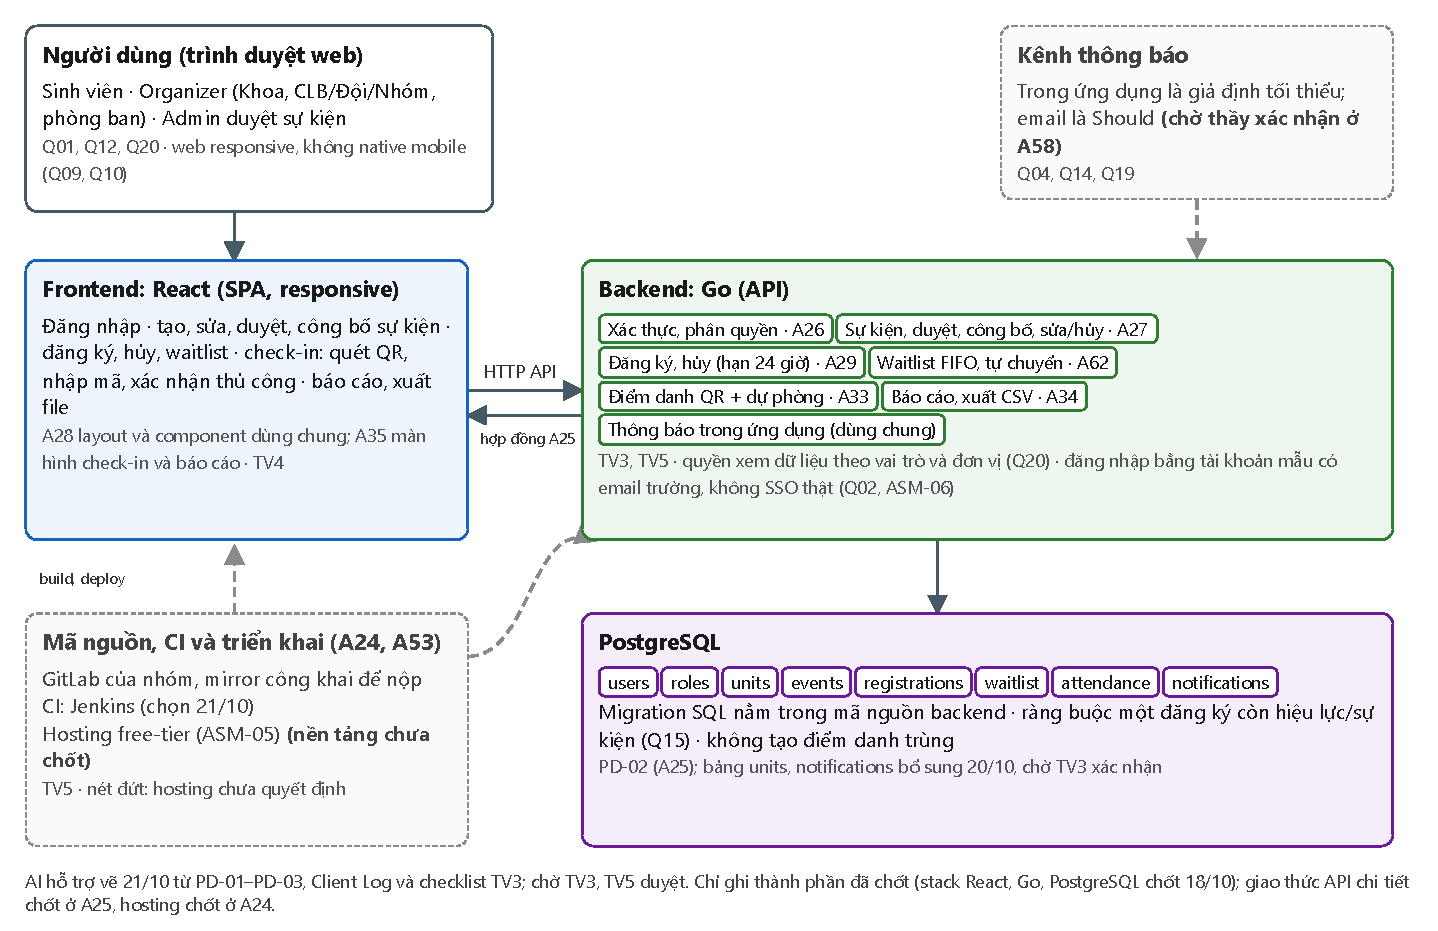
\includegraphics[width=\linewidth]{image/architecture.pdf}
\caption{Kiến trúc kỹ thuật React -- Go -- PostgreSQL và activity tương ứng}
\label{fig:architecture}
\end{figure}

\kiemtra{Hình~\ref{fig:architecture} do AI hỗ trợ vẽ ngày 21/10 từ PD-01 đến PD-03, Client Log và checklist TV3; chờ TV3, TV5 duyệt (nhất là phân chia module backend và bảng PostgreSQL).}

\subsection*{Kế hoạch giao tiếp}
\begin{itemize}
  \item \textbf{Với client:} qua email; TV1 là đầu mối, gom câu hỏi trước khi gửi; client không cam kết thời gian phản hồi (P02, P05). Mọi trao đổi ghi vào Client Log kèm mốc thời gian.
  \item \textbf{Trong nhóm:} dùng chat để báo tiến độ và vướng mắc bất đồng bộ; check-in 3 dòng vào thứ Tư/thứ Năm. TV1 tổng hợp tiến độ hằng tuần.
  \item \textbf{Công cụ theo dõi:} board Jira theo dõi công việc theo mã activity; Sheet Master ghi thời gian và bằng chứng.
  \item \textbf{Họp định kỳ:} 15h00 Chủ nhật hằng tuần, để rà soát time tracking, chốt weekly log, review chéo tài liệu và chuẩn bị cho viva.
  \item \textbf{Họp bất thường:} thêm khi gặp một trong các ngưỡng ở mục~\ref{sec:1-5}.
\end{itemize}

\subsection*{Tiêu chuẩn và quy trình}
\begin{itemize}
  \item \textbf{Git:} mỗi công việc một nhánh; Pull Request ghi mã công việc, nội dung thay đổi, cách kiểm tra; ít nhất một thành viên khác review trước khi vào \texttt{main}.
  \item \textbf{Bảo mật:} không đưa mật khẩu, khóa truy cập hoặc dữ liệu thật của sinh viên lên repo.
  \item \textbf{Định nghĩa hoàn thành:} code chạy được, đáp ứng yêu cầu công việc, đã kiểm tra phù hợp và đã review; tài liệu ghi rõ người thực hiện, nguồn thông tin và các điểm còn là giả định. Mức kiểm thử xác định theo từng tính năng, không bắt buộc unit test đầy đủ cho mọi công việc.
  \item \textbf{Giao diện:} ưu tiên hiển thị tốt trên điện thoại (mobile-first) cho màn hình điểm danh; dùng thư viện UI component có sẵn cho biểu mẫu và bảng để rút ngắn thời gian; giao diện dùng React (nhóm chốt stack ngày 18/10).
\end{itemize}
\todo{Bổ sung: chuẩn đặt tên (nhánh, file, mã activity), chuẩn coding/tài liệu, quy trình change request.}

\section{Đặc điểm dự án, rủi ro cấp cao và lựa chọn vòng đời}
\label{sec:1-8}

\subsection*{Đặc điểm dự án}
Dự án được quản lý theo sản phẩm (product-based): nhóm có thể mô tả, bàn giao và kiểm tra một ứng dụng web với các luồng nghiệp vụ cụ thể. Các đặc điểm ảnh hưởng đến cách tiếp cận:
\begin{itemize}
  \item Thời hạn môn học cố định, nhóm nhỏ.
  \item Workflow và các quy tắc duyệt, hủy, waitlist đã được client xác nhận (vòng 1 và vòng 2); vẫn có khả năng phát sinh thay đổi do change event (Q17).
  \item Chưa có số liệu vận hành thực tế; mọi chỉ tiêu tải và lợi ích định lượng phải ghi là giả định.
\end{itemize}

\subsection*{Lựa chọn vòng đời}
\begingroup\tblsetup\tblzebra
\begin{longtable}{L{3.0cm}L{11.0cm}}
\caption{So sánh các cách tiếp cận vòng đời}\label{tab:lifecycle}\\
\toprule
\rowcolor{tblheadbg}\textbf{Cách tiếp cận} & \textbf{Đánh giá theo dự án} \\
\midrule
\endfirsthead
\toprule
\rowcolor{tblheadbg}\textbf{Cách tiếp cận} & \textbf{Đánh giá theo dự án} \\
\midrule
\endhead
\bottomrule
\endlastfoot
Waterfall & Tạo trình tự tài liệu rõ nhưng phản hồi muộn khi quy tắc chi tiết thay đổi \\
Scrum đầy đủ & Có vòng phản hồi thường xuyên nhưng nhóm chưa thiết lập đầy đủ vai trò, sự kiện và quản lý backlog theo Scrum \\
Incremental delivery & \textbf{Chọn:} lập kế hoạch theo các mốc của môn học (Progress Check, demo), giao từng phần workflow chạy được, kiểm thử và điều chỉnh theo phản hồi \\
\end{longtable}
\endgroup

Nhóm chọn product-based với incremental delivery: baseline cố định, giao sản phẩm theo 2 increment. Thứ tự tăng trưởng theo phụ thuộc nghiệp vụ:
\begin{enumerate}
  \item Vai trò, tạo sự kiện, duyệt và công bố.
  \item Đăng ký, hủy, giới hạn số chỗ và tự động chuyển người đầu danh sách chờ.
  \item Điểm danh bằng QR cùng phương án nhập mã hoặc xác nhận thủ công.
  \item Báo cáo và xuất dữ liệu.
\end{enumerate}
Phân quyền và bảo vệ dữ liệu được kiểm tra trong mọi đợt. Đây là thứ tự phụ thuộc; ranh giới chính xác giữa hai increment sẽ được cập nhật ở Baseline V1.0. Không đưa check-out, SSO thật, app native hoặc tích hợp điểm rèn luyện vào cam kết kỹ thuật. Client liên hệ được bằng email nhưng không cam kết thời gian phản hồi.

Trong mỗi increment, tiến độ được theo dõi bằng sprint hằng tuần trên Jira (Bảng~\ref{tab:tools}); đây là cách chia nhỏ việc để theo dõi, không phải áp dụng Scrum đầy đủ.

\subsection*{Rủi ro cấp cao}
Bảng~\ref{tab:risk-high} liệt kê các rủi ro cấp dự án đã nhận diện và hướng xử lý ở mức cách tiếp cận.

Các rủi ro trong bảng ảnh hưởng tới toàn dự án thay vì một activity riêng lẻ; rủi ro gắn với từng activity ở mục~\ref{sec:2-8}. P (xác suất) và I (tác động) chấm theo thang 1--5, Exposure = P $\times$ I. Số liệu lấy từ Risk Register của Sheet master (bản export 22/10): P, I ban đầu do AI đề xuất ngày 13/10, owner xác nhận ở cột \enquote{Người duyệt}. Rủi ro R10 (Milestone 1 sớm hơn kế hoạch) đã xảy ra ngày 02/10 và chuyển thành issue I01 (mục~\ref{sec:3-4}); việc chưa có số liệu sử dụng thực tế được xử lý bằng giả định ASM-02 (Bảng~\ref{tab:assumptions}), không đưa vào sổ rủi ro.

\kiemtra{R02, R03, R05, R07, R15 thay cho bốn dòng mô tả chung của bản M1 (quy tắc nghiệp vụ tự đề xuất, thời hạn cố định, chưa có dữ liệu thực tế, giới hạn thời gian và kinh nghiệm); nhóm xác nhận cách thay này. R03, R05, R07, R15 do TV1 làm owner, TV1 duyệt ngày 22/10.}

\begingroup\tblsetup\tblzebra
\begin{longtable}{L{0.8cm}L{2.6cm}L{0.3cm}L{0.3cm}L{0.9cm}L{1.3cm}L{3.0cm}L{2.4cm}L{1.0cm}}
\caption{Rủi ro cấp cao}\label{tab:risk-high}\\
\toprule
\rowcolor{tblheadbg}\textbf{ID} & \textbf{Mô tả} & \textbf{P} & \textbf{I} & \textbf{Exp.} & \textbf{Owner} & \textbf{Giảm thiểu} & \textbf{Dự phòng} & \textbf{TT} \\
\midrule
\endfirsthead
\toprule
\rowcolor{tblheadbg}\textbf{ID} & \textbf{Mô tả} & \textbf{P} & \textbf{I} & \textbf{Exp.} & \textbf{Owner} & \textbf{Giảm thiểu} & \textbf{Dự phòng} & \textbf{TT} \\
\midrule
\endhead
\bottomrule
\endlastfoot
R15 & Lịch vượt Progress Check 09/11 và demo 07/12 vì năng lực 14h/tuần (E01) và nhiều activity do một người làm. Lịch A21 (21/10) chỉ vừa kịp 07/12, không còn ngày dự trữ; Progress Check 09/11 chưa có QR check-in & 4 & 4 & 16 & TV1 & Baseline V1.0 chỉ gồm Must; A34 không chặn A37; thêm owner cho A24, A31, A35; hỏi thầy phạm vi tối thiểu (A58) & Thu hẹp phạm vi theo thứ tự Could rồi Should & Open \\
R05 & Change event của giảng viên làm tăng scope đáng kể; nội dung không báo trước (Q17) & 5 & 3 & 15 & TV1 & Contingency A38 (30h) là quỹ ngoài chuỗi (L6 = B), dùng giờ dư của TV2--TV5; template Change Request sẵn & Cắt Should rồi Could; lập Baseline V2.0 & Open \\
R02 & Ước lượng thấp hơn thực tế do nhóm thiếu kinh nghiệm & 4 & 3 & 12 & TV3 & Tính cả AI review/test/sửa lỗi trong estimate; so sánh actual hằng tuần; báo PM khi vượt; CP2 18/10: ý kiến trái chiều về estimate implement/testing, chưa có số thay thế; PM giữ số 20/10, so actual hằng tuần & Cân bằng tài nguyên/reserve hoặc đổi scope theo quy trình & Open \\
R03 & Thành viên bận thi giữa kỳ hoặc môn khác; tuần nghỉ chỉ khoảng 6h/người (E02) & 4 & 3 & 12 & TV1 & Thu lịch thi sớm (A50); tuần nghỉ chỉ giao việc nhẹ & Hoán đổi việc, dùng float trước 20/10 & Open \\
R07 & Thành viên không đóng góp hoặc rời nhóm & 2 & 5 & 10 & TV1 & Owner rõ ràng; theo dõi time tracking và check-in thứ Tư/thứ Năm & Phân lại việc, báo giảng viên & Open \\
\end{longtable}
\endgroup

\chapter{Lập kế hoạch và Baseline (Task 2)}
\label{chap:task2}

% Kiểu nút dùng chung cho các sơ đồ PBS, PFD và mạng hoạt động trong chương này.
\tikzset{
  act/.style={draw, rounded corners, align=center, font=\scriptsize, text width=2.6cm, inner sep=3pt, minimum height=1cm},
  crit/.style={act, fill=red!12, draw=red!70!black, thick},
  ghost/.style={act, dashed, fill=gray!10}
}

\section{Cấu trúc phân rã sản phẩm (PBS)}
\label{sec:2-1}
PBS (Hình~\ref{fig:pbs}) chia sản phẩm của dự án thành hai nhánh: sản phẩm quản lý (M) phục vụ việc điều hành và nộp bài, và sản phẩm kỹ thuật (S) là những gì được xây dựng và bàn giao. Mỗi nút có mã để truy vết sang activity ở mục~\ref{sec:2-4}. Các module phần mềm (S31--S36) bám theo chuỗi cốt lõi mà client ưu tiên: quản lý sự kiện, đăng ký và danh sách chờ, điểm danh, báo cáo (Q08).

\begin{figure}[H]
\centering
\resizebox{\linewidth}{!}{%
\hyphenpenalty=10000 \exhyphenpenalty=10000\relax
\begin{tikzpicture}[>={Stealth[length=2mm]}]
  \node[act,text width=4.4cm] (M1) at (8.4,0.00) {\textbf{M1} Project Definition};
  \node[act,text width=4.4cm] (M2) at (8.4,-1.20) {\textbf{M2} Project Baseline};
  \node[act,text width=4.4cm] (M3) at (8.4,-2.40) {\textbf{M3} Monitoring \& Change Records};
  \node[act,text width=4.4cm] (M4) at (8.4,-3.60) {\textbf{M4} Final Report \& Closure};
  \node[act,text width=3.6cm] (M) at (3.6,-1.80) {\textbf{M} Management Products};
  \node[act,text width=4.4cm] (S1) at (8.4,-4.80) {\textbf{S1} Validated Scope \& Requirements};
  \node[act,text width=5.8cm] (S21) at (15.2,-6.00) {\textbf{S21} Database Design};
  \node[act,text width=5.8cm] (S22) at (15.2,-7.20) {\textbf{S22} API Contract};
  \node[act,text width=4.4cm] (S2) at (8.4,-6.60) {\textbf{S2} System Design};
  \node[act,text width=5.8cm] (S31) at (15.2,-8.40) {\textbf{S31} Authentication \& Authorization};
  \node[act,text width=5.8cm] (S32) at (15.2,-9.60) {\textbf{S32} Event Management};
  \node[act,text width=5.8cm] (S33) at (15.2,-10.80) {\textbf{S33} Registration \& Waitlist};
  \node[act,text width=5.8cm] (S34) at (15.2,-12.00) {\textbf{S34} Check-in \& Attendance};
  \node[act,text width=5.8cm] (S35) at (15.2,-13.20) {\textbf{S35} Reporting \& Export};
  \node[act,text width=5.8cm] (S36) at (15.2,-14.40) {\textbf{S36} User Interface};
  \node[act,text width=4.4cm] (S3) at (8.4,-11.40) {\textbf{S3} Software Products};
  \node[act,text width=5.8cm] (S41) at (15.2,-15.60) {\textbf{S41} Test Specification};
  \node[act,text width=5.8cm] (S42) at (15.2,-16.80) {\textbf{S42} Tested Integrated System};
  \node[act,text width=4.4cm] (S4) at (8.4,-16.20) {\textbf{S4} Test Products};
  \node[act,text width=5.8cm] (S51) at (15.2,-18.00) {\textbf{S51} Deployed System};
  \node[act,text width=5.8cm] (S52) at (15.2,-19.20) {\textbf{S52} Handover Documentation};
  \node[act,text width=4.4cm] (S5) at (8.4,-18.60) {\textbf{S5} Release Products};
  \node[act,text width=3.6cm] (S) at (3.6,-11.70) {\textbf{S} Specialist Products};
  \node[act,text width=3.4cm] (P0) at (-1.6,-6.75) {\textbf{P0} University Event Registration System};
  \draw[->] (M.east) to[out=0,in=180] (M1.west);
  \draw[->] (M.east) to[out=0,in=180] (M2.west);
  \draw[->] (M.east) to[out=0,in=180] (M3.west);
  \draw[->] (M.east) to[out=0,in=180] (M4.west);
  \draw[->] (S.east) to[out=0,in=180] (S1.west);
  \draw[->] (S2.east) to[out=0,in=180] (S21.west);
  \draw[->] (S2.east) to[out=0,in=180] (S22.west);
  \draw[->] (S.east) to[out=0,in=180] (S2.west);
  \draw[->] (S3.east) to[out=0,in=180] (S31.west);
  \draw[->] (S3.east) to[out=0,in=180] (S32.west);
  \draw[->] (S3.east) to[out=0,in=180] (S33.west);
  \draw[->] (S3.east) to[out=0,in=180] (S34.west);
  \draw[->] (S3.east) to[out=0,in=180] (S35.west);
  \draw[->] (S3.east) to[out=0,in=180] (S36.west);
  \draw[->] (S.east) to[out=0,in=180] (S3.west);
  \draw[->] (S4.east) to[out=0,in=180] (S41.west);
  \draw[->] (S4.east) to[out=0,in=180] (S42.west);
  \draw[->] (S.east) to[out=0,in=180] (S4.west);
  \draw[->] (S5.east) to[out=0,in=180] (S51.west);
  \draw[->] (S5.east) to[out=0,in=180] (S52.west);
  \draw[->] (S.east) to[out=0,in=180] (S5.west);
  \draw[->] (P0.east) to[out=0,in=180] (M.west);
  \draw[->] (P0.east) to[out=0,in=180] (S.west);
\end{tikzpicture}}
\caption{Cấu trúc phân rã sản phẩm (PBS)}
\label{fig:pbs}
\end{figure}

Sơ đồ là kết quả A15 (TV3, TV5); bộ mã M/S là mã sản phẩm chính thức của dự án (TV1 chốt 20/10).

\section{Mô tả sản phẩm (Product Descriptions)}
\label{sec:2-2}
Năm Product Description dưới đây mô tả các sản phẩm quyết định việc nghiệm thu và kiểm thử: S1, S21, S34, S41, S51 (mã theo PBS ở mục~\ref{sec:2-1}). Mỗi PD gồm các trường định danh, mục đích, nguồn tạo ra, thành phần, định dạng, tiêu chuẩn liên quan, tiêu chí chất lượng và phương pháp kiểm tra. Nội dung lấy từ tab Product Description của Sheet master; các PD được thành viên duyệt ngày 14/10, bổ sung ngày 20/10 theo phản hồi Q12, Q19, Q20 và stack đã chốt (React, Go, PostgreSQL).

\subsection*{PD-01 -- S1 Validated Scope \& Requirements}
\noindent\textit{TV2 duyệt 14/10; bổ sung Q12, Q19, Q20 ngày 20/10.}

\begingroup\tblsetup\tblzebra
\begin{longtable}{L{3.4cm}L{11.6cm}}
\caption{PD-01 -- S1 Validated Scope \& Requirements}\label{tab:pd-01}\\
\toprule
\rowcolor{tblheadbg}\textbf{Trường} & \textbf{Nội dung} \\
\midrule
\endfirsthead
\toprule
\rowcolor{tblheadbg}\textbf{Trường} & \textbf{Nội dung} \\
\midrule
\endhead
\bottomrule
\endlastfoot
Định danh & S1 Đặc tả yêu cầu (Validated Scope \& Requirements) \\
Mục đích & Mô tả đầy đủ yêu cầu chức năng và phi chức năng đã được client xác nhận, làm đầu vào cho thiết kế, kiểm thử và Baseline V1.0 \\
Nguồn tạo ra (derivation) & Client Interaction Log (Q01–Q20), scope và MoE (A07), giả định ASM-01 đến ASM-07 \\
Thành phần & Danh sách REQ-01 đến REQ-21 có mức MoSCoW và tiêu chí chấp nhận; ràng buộc phi chức năng; giả định và loại trừ; quy tắc nghiệp vụ đã xác nhận (hạn hủy 24 giờ, waitlist FIFO, một đăng ký còn hiệu lực/sinh viên/sự kiện; Organizer không tự duyệt sự kiện mình tạo, Admin duyệt (Q12); Organizer sửa/hủy sự kiện sau công bố, đổi thời gian/địa điểm phải thông báo (Q19); quyền xem dữ liệu theo vai trò và đơn vị (Q20)) \\
Định dạng & Markdown trong \texttt{docs/task2}, xuất sang báo cáo mục 1.4 \\
Tiêu chuẩn liên quan & Mỗi requirement có mã duy nhất và truy ngược được về câu trả lời của client hoặc assumption có mã \\
Tiêu chí chất lượng & 100\% requirement Must có tiêu chí chấp nhận kiểm tra được; 100\% truy ngược được về Client Log hoặc assumption; không có mâu thuẫn giữa bảng MoSCoW và báo cáo \\
Phương pháp và người kiểm tra & Review chéo bởi TV1 theo checklist CP2; client đã xác nhận scope ở Q10 và Q11 \\
\end{longtable}
\endgroup

\subsection*{PD-02 -- S21 Database Design}
\noindent\textit{TV4, TV3 duyệt 14/10; bổ sung bảng units, notifications và stack ngày 20/10, chờ TV3 xác nhận.}

\begingroup\tblsetup\tblzebra
\begin{longtable}{L{3.4cm}L{11.6cm}}
\caption{PD-02 -- S21 Database Design}\label{tab:pd-02}\\
\toprule
\rowcolor{tblheadbg}\textbf{Trường} & \textbf{Nội dung} \\
\midrule
\endfirsthead
\toprule
\rowcolor{tblheadbg}\textbf{Trường} & \textbf{Nội dung} \\
\midrule
\endhead
\bottomrule
\endlastfoot
Định danh & S21 Thiết kế cơ sở dữ liệu (ERD và schema) \\
Mục đích & Mô hình dữ liệu đáp ứng mọi requirement Must và các quy tắc nghiệp vụ đã xác nhận \\
Nguồn tạo ra (derivation) & S1 Validated Scope \& Requirements; ASM-02 (quy mô) \\
Thành phần & ERD; định nghĩa bảng users, roles, units (đơn vị tổ chức, Q01, Q20), events, registrations, waitlist, attendance, notifications (thông báo trong ứng dụng, Q14, Q19); khóa, ràng buộc, chỉ mục; trạng thái sự kiện gồm Cancelled (Q19); waitlist có thứ tự FIFO, tự chuyển đầu waitlist và tạo thông báo (Q14); đăng ký còn hiệu lực hoặc đã hủy, lưu thời điểm để đăng ký lại vào cuối waitlist (Q15) \\
Định dạng & Sơ đồ ERD; file migration SQL cho PostgreSQL trong mã nguồn backend (Go) \\
Tiêu chuẩn liên quan & Chuẩn hóa tới 3NF trừ khi có lý do ghi rõ; tên bảng và cột snake\_case \\
Tiêu chí chất lượng & Mọi requirement Must ánh xạ được vào thực thể; ràng buộc không đăng ký trùng và không vượt số chỗ được thực thi ở mức database; tự chuyển đầu waitlist đúng một lần, không chuyển trùng; thông báo lỗi vẫn giữ đăng ký chính thức; test đồng thời 100 lượt đăng ký không vượt chỗ \\
Phương pháp và người kiểm tra & Review bởi TV3 và TV4 (frontend dùng được); test FIFO và đồng thời, test tích hợp với dữ liệu mẫu 500 lượt đăng ký \\
\end{longtable}
\endgroup

\subsection*{PD-03 -- S34 Check-in \& Attendance}
\noindent\textit{TV4 duyệt 14/10; bổ sung stack và quyền điểm danh 20/10.}

\begingroup\tblsetup\tblzebra
\begin{longtable}{L{3.4cm}L{11.6cm}}
\caption{PD-03 -- S34 Check-in \& Attendance}\label{tab:pd-03}\\
\toprule
\rowcolor{tblheadbg}\textbf{Trường} & \textbf{Nội dung} \\
\midrule
\endfirsthead
\toprule
\rowcolor{tblheadbg}\textbf{Trường} & \textbf{Nội dung} \\
\midrule
\endhead
\bottomrule
\endlastfoot
Định danh & S34 Module điểm danh (Check-in \& Attendance) \\
Mục đích & Ghi nhận người tham dự nhanh và chính xác tại sự kiện, kể cả khi QR không dùng được \\
Nguồn tạo ra (derivation) & S33 Registration \& Waitlist; kết quả spike A20; Q03 \\
Thành phần & Sinh mã QR cho đăng ký; màn hình quét; nhập mã hoặc xác nhận thủ công; chặn điểm danh trùng; lưu thời điểm; không check-out \\
Định dạng & Mã nguồn giao diện quét (React) và API điểm danh (Go), chạy trên bản deploy \\
Tiêu chuẩn liên quan & Hoạt động trên trình duyệt điện thoại, mobile-first, không cần cài ứng dụng \\
Tiêu chí chất lượng & Median thời gian điểm danh $\le$ 5 giây trong môi trường test của nhóm (O2); không tạo bản ghi điểm danh trùng; phương án thủ công cập nhật giống QR; chỉ Organizer của sự kiện hoặc Admin được điểm danh (Q20) \\
Phương pháp và người kiểm tra & Test trên ít nhất 3 thiết bị thật; test case T-CI-01 đến T-CI-05 (đề xuất, mã chốt ở A22); review bởi TV2 \\
\end{longtable}
\endgroup

\subsection*{PD-04 -- S41 Test Specification}
\noindent\textit{TV2 duyệt 14/10.}

\begingroup\tblsetup\tblzebra
\begin{longtable}{L{3.4cm}L{11.6cm}}
\caption{PD-04 -- S41 Test Specification}\label{tab:pd-04}\\
\toprule
\rowcolor{tblheadbg}\textbf{Trường} & \textbf{Nội dung} \\
\midrule
\endfirsthead
\toprule
\rowcolor{tblheadbg}\textbf{Trường} & \textbf{Nội dung} \\
\midrule
\endhead
\bottomrule
\endlastfoot
Định danh & S41 Đặc tả kiểm thử (test plan và test case) \\
Mục đích & Mô tả kế hoạch và test case để kiểm tra các requirement; là bằng chứng cho Task 3.5 và đầu vào cho UAT. Kết quả chạy test được lưu riêng. \\
Nguồn tạo ra (derivation) & S1 Validated Scope \& Requirements; quality plan (A22) \\
Thành phần & Chiến lược test theo mức (unit, integration, e2e, UAT); test case có mã gắn với requirement; dữ liệu test; tiêu chí pass/fail; nơi lưu kết quả \\
Định dạng & Markdown trong \texttt{docs/quality} và test tự động trong \texttt{src/} \\
Tiêu chuẩn liên quan & Mã test theo quy ước T-nhóm-số (ví dụ T-REG-01), gắn với REQ \\
Tiêu chí chất lượng & 100\% requirement Must có ít nhất một test case; mỗi test case có kết quả kỳ vọng đo được; 100\% test đã chạy được ghi kết quả \\
Phương pháp và người kiểm tra & Review bởi TV1 và TV4; kết quả chạy lưu và liên kết từ ma trận truy vết \\
\end{longtable}
\endgroup

\subsection*{PD-05 -- S51 Deployed System}
\noindent\textit{TV2 duyệt 14/10.}

\begingroup\tblsetup\tblzebra
\begin{longtable}{L{3.4cm}L{11.6cm}}
\caption{PD-05 -- S51 Deployed System}\label{tab:pd-05}\\
\toprule
\rowcolor{tblheadbg}\textbf{Trường} & \textbf{Nội dung} \\
\midrule
\endfirsthead
\toprule
\rowcolor{tblheadbg}\textbf{Trường} & \textbf{Nội dung} \\
\midrule
\endhead
\bottomrule
\endlastfoot
Định danh & S51 Hệ thống đã triển khai \\
Mục đích & Sản phẩm chạy được để client nghiệm thu và nhóm demo \\
Nguồn tạo ra (derivation) & S42 Tested Integrated System (toàn bộ module S31 đến S36) \\
Thành phần & Ứng dụng đang chạy; database có dữ liệu mẫu (500 lượt đăng ký); 3 tài khoản demo cho Student, Organizer, Admin (ASM-06); README hướng dẫn chạy \\
Định dạng & URL bản deploy và mã nguồn trong repo (bản mirror công khai) \\
Tiêu chuẩn liên quan & Chạy trên trình duyệt phổ biến và điện thoại; không lưu mật khẩu hay dữ liệu thật trong repo \\
Tiêu chí chất lượng & Luồng tạo sự kiện, duyệt, đăng ký, waitlist, check-in, báo cáo chạy không lỗi nghiêm trọng; người ngoài nhóm dựng lại được theo README trong dưới 30 phút \\
Phương pháp và người kiểm tra & Regression test A39; UAT A41; review bởi TV5 \\
\end{longtable}
\endgroup

\kiemtra{PD-02: phần bổ sung ngày 20/10 (bảng units, notifications; migration PostgreSQL) chờ TV3 xác nhận. PD-03: mã test T-CI-01 đến T-CI-05 là đề xuất, mã chính thức chốt ở A22.}

\section{Sơ đồ luồng sản phẩm (PFD)}
\label{sec:2-3}
PFD (Hình~\ref{fig:pfd}) cho biết sản phẩm nào là đầu vào để tạo ra sản phẩm nào. Đây là quan hệ dẫn xuất giữa sản phẩm, không phải thứ tự công việc; thứ tự công việc nằm ở mạng hoạt động (mục~\ref{sec:2-4}).

\begin{figure}[H]
\centering
\resizebox{0.95\linewidth}{!}{%
\hyphenpenalty=10000 \exhyphenpenalty=10000\relax
\begin{tikzpicture}[>={Stealth[length=2mm]}]
  \node[act,text width=3.4cm] (REQ) at (6.00,0.00) {Validated Scope \& Requirements};
  \node[act,text width=3.4cm] (DB) at (0.00,-1.90) {Database Design};
  \node[act,text width=3.4cm] (API) at (4.00,-1.90) {API Contract};
  \node[act,text width=3.4cm] (TEST) at (8.00,-1.90) {Test Specification};
  \node[act,text width=3.4cm] (UI) at (12.00,-1.90) {User Interface};
  \node[act,text width=3.4cm] (AUTH) at (8.00,-3.80) {Authentication \& Authorization};
  \node[act,text width=3.4cm] (EVENT) at (2.40,-3.80) {Event Management};
  \node[act,text width=3.4cm] (REG) at (2.40,-5.70) {Registration \& Waitlist};
  \node[act,text width=3.4cm] (CHECK) at (2.40,-7.60) {Check-in \& Attendance};
  \node[act,text width=3.4cm] (REPORT) at (2.40,-9.50) {Reporting \& Export};
  \node[act,text width=3.4cm] (SYS) at (2.40,-11.40) {Tested Integrated System};
  \node[act,text width=3.4cm] (DEPLOY) at (2.40,-13.30) {Deployed System};
  \node[act,text width=3.4cm] (HAND) at (2.40,-15.20) {Handover Documentation};
  \draw[->] (REQ) -- (DB);
  \draw[->] (REQ) -- (API);
  \draw[->] (REQ) -- (TEST);
  \draw[->] (REQ) -- (UI);
  \draw[->] (DB) -- (EVENT);
  \draw[->] (API) -- (EVENT);
  \draw[->] (DB) -- (AUTH);
  \draw[->] (API) -- (AUTH);
  \draw[->] (EVENT) -- (REG);
  \draw[->] (REG) -- (CHECK);
  \draw[->] (CHECK) -- (REPORT);
  \draw[->] (REPORT) -- (SYS);
  \draw[->] (SYS) -- (DEPLOY);
  \draw[->] (DEPLOY) -- (HAND);
  \draw[->] (REG.west) to[out=180,in=180,looseness=1.4] (REPORT.west);
  \draw[->] (EVENT.west) to[out=180,in=180,looseness=1] (SYS.west);
  \draw[->] (REG.west) to[out=180,in=180,looseness=1.2] (SYS.west);
  \draw[->] (CHECK.west) to[out=180,in=180,looseness=1.4] (SYS.west);
  \draw[->] (AUTH.east) to[out=0,in=0,looseness=1] (SYS.east);
  \draw[->] (TEST.east) to[out=0,in=0,looseness=1] (SYS.east);
  \draw[->] (UI.east) to[out=0,in=0,looseness=1] (SYS.east);
\end{tikzpicture}}
\caption{Sơ đồ luồng sản phẩm (PFD)}
\label{fig:pfd}
\end{figure}

Sơ đồ là kết quả A15 (TV3, TV5).

\section{Mạng hoạt động}
\label{sec:2-4}
Activity được suy ra từ PFD: mỗi sản phẩm trong PFD có ít nhất một activity tạo ra nó. Tên activity theo dạng động từ cộng danh từ; quan hệ phụ thuộc là finish-to-start; các mốc theo lịch môn học (hỏi client, duyệt baseline, Progress Check, UAT, demo) được đặt ràng buộc không bắt đầu trước ngày cố định. Mạng được chia làm ba hình: lập kế hoạch đến chốt baseline (Hình~\ref{fig:net-a}), Increment 1 và Increment 2 đến Progress Check (Hình~\ref{fig:net-b}), kiểm thử Increment 2 đến demo (Hình~\ref{fig:net-c}). Mỗi nút ghi effort, thời lượng CPM, ngày theo lịch đã san tải, người làm và float CPM (mục~\ref{sec:2-11}). Nút viền đỏ là đường găng sau san tải; nút nét đứt là activity thuộc hình khác; cạnh nét đứt xanh là phụ thuộc được sửa ở L8--L11 (A21, A50).

\begin{figure}[p]
\centering
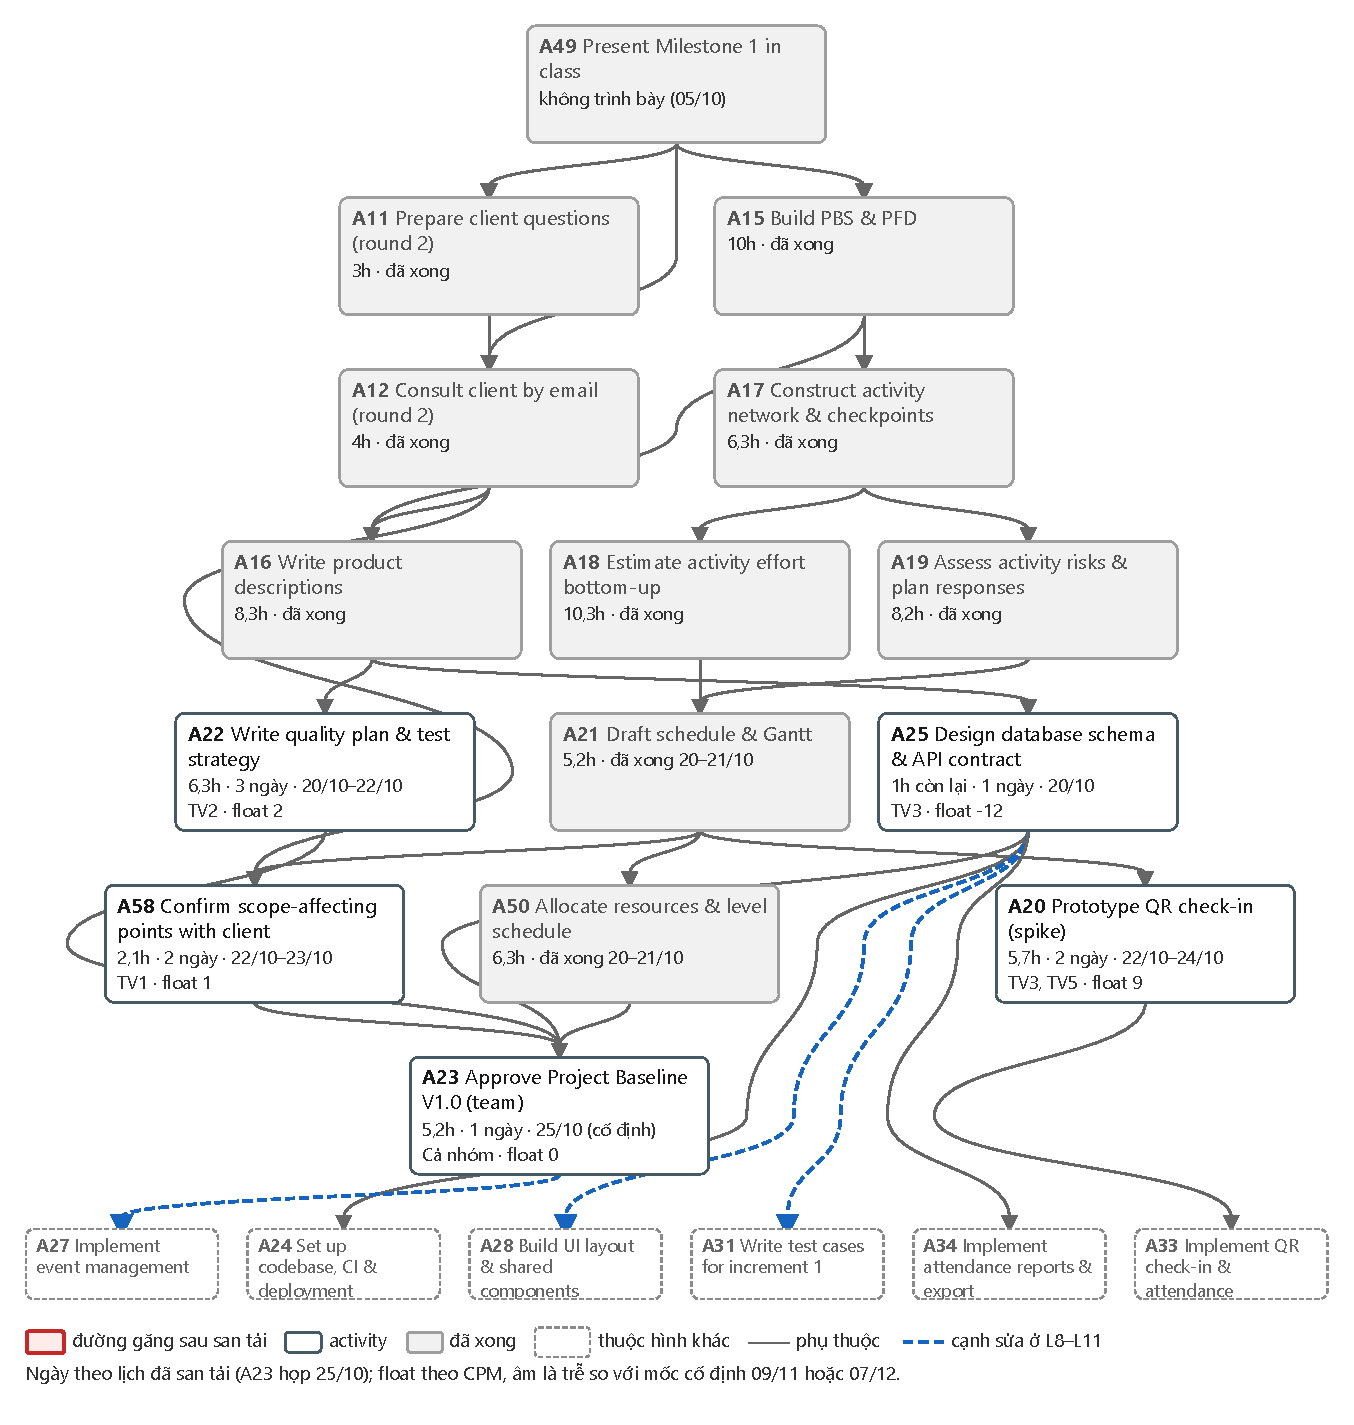
\includegraphics[width=\linewidth,height=0.9\textheight,keepaspectratio]{image/network-a.pdf}
\caption{Mạng hoạt động -- từ PBS/PFD đến chốt Baseline V1.0 (A23, 25/10)}
\label{fig:net-a}
\end{figure}

\begin{figure}[p]
\centering
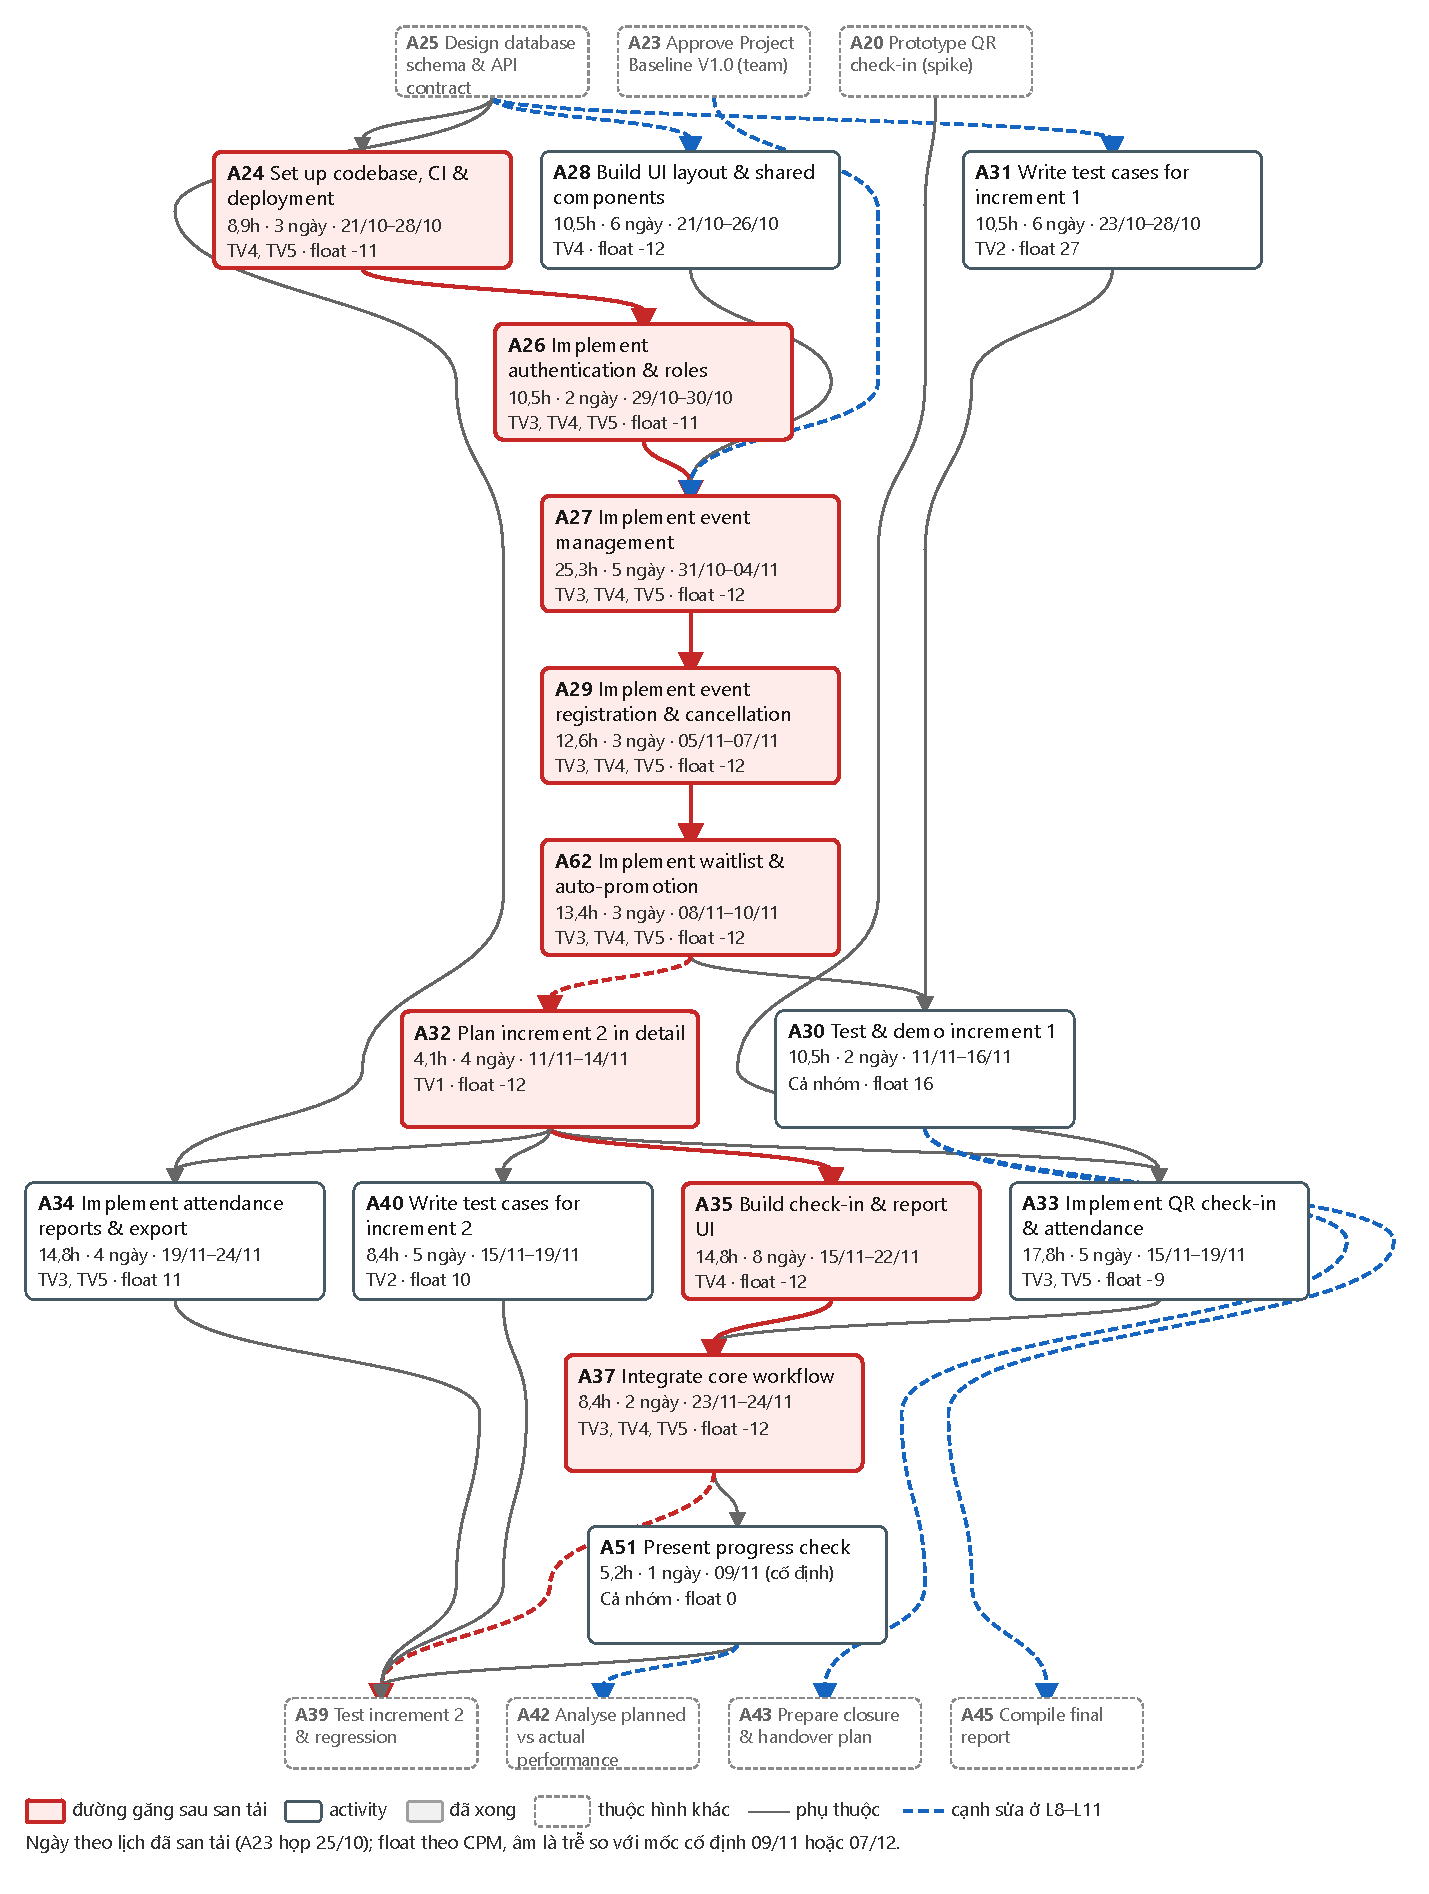
\includegraphics[width=\linewidth,height=0.9\textheight,keepaspectratio]{image/network-b.pdf}
\caption{Mạng hoạt động -- Increment 1 và Increment 2 đến Progress Check (A51, 09/11)}
\label{fig:net-b}
\end{figure}

\begin{figure}[p]
\centering
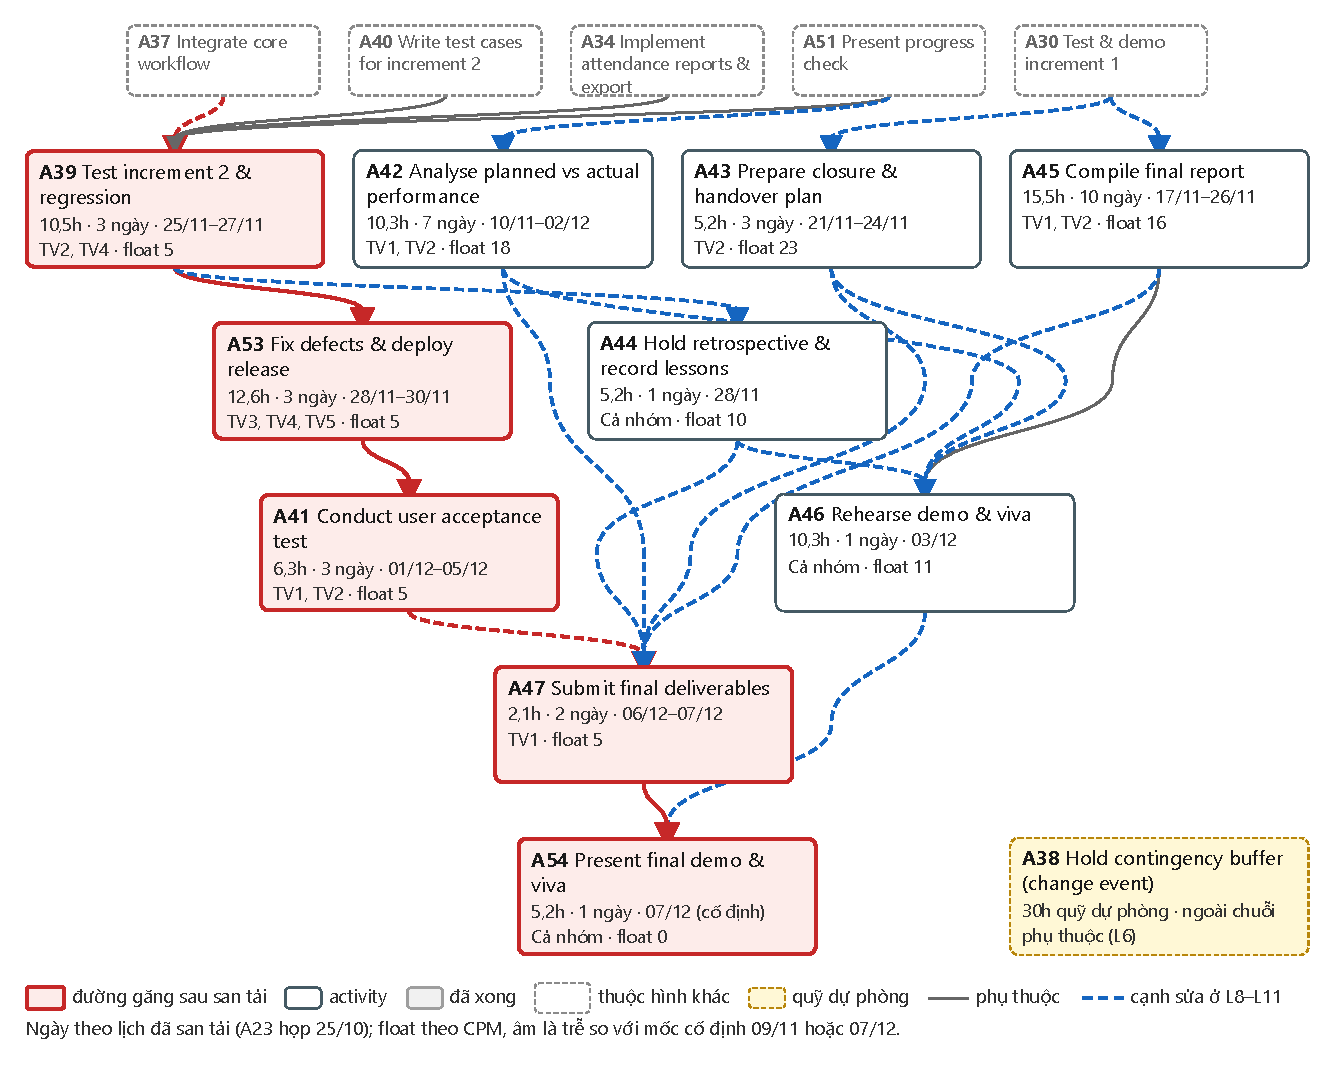
\includegraphics[width=\linewidth,height=0.9\textheight,keepaspectratio]{image/network-c.pdf}
\caption{Mạng hoạt động -- kiểm thử Increment 2, nghiệm thu, đóng dự án và demo; A38 là quỹ dự phòng ngoài chuỗi}
\label{fig:net-c}
\end{figure}

Các activity xuyên suốt A36 (giám sát tiến độ) và A57 (rà soát truy vết) là hammock chạy nền từ sau A23 đến 07/12 nên không vẽ trong sơ đồ; chúng có trên Gantt (Hình~\ref{fig:gantt}). Đường găng trong sơ đồ là kết quả CPM và san tải ở A21, A50.

Khi đối chiếu PFD với mạng hoạt động, nhóm phát hiện các điểm lệch dưới đây; PM chốt cách xử lý từ 12 đến 15/10 và nhóm duyệt tại CP2 ngày 18/10.
\begin{itemize}
  \item \textbf{Báo cáo và điểm danh:} PFD cho điểm danh đi trước báo cáo. Để không làm trễ Progress Check 09/11, A34 (báo cáo) làm gối đầu A33 (điểm danh), bắt đầu sau A32 và A25 trên dữ liệu mẫu; A37 chỉ gồm A33 và A35; báo cáo được tích hợp và kiểm với dữ liệu điểm danh thật ở A39. Đây là lệch khỏi PFD có chủ đích. PM chọn ngày 13/10 trong các phương án AI đề xuất, TV3 xác nhận khả thi ngày 14/10.
  \item \textbf{Danh sách chờ:} client xác nhận danh sách chờ với tự động chuyển người là một phần của workflow cốt lõi (Q04, Q08). Activity đăng ký cũ được tách thành A29 (đăng ký, hủy) và A62 (danh sách chờ, tự động chuyển, thông báo); quy tắc chi tiết đã được client xác nhận ở vòng 2 (Q14, Q15).
  \item \textbf{Sửa hoặc hủy sự kiện đã công bố:} yêu cầu mới từ phản hồi 08/10 (Q19), ảnh hưởng A27 (quản lý sự kiện) và A29 (hủy đăng ký theo sự kiện). Phần sửa, hủy sự kiện và thông báo được tính trong A27, không tính trùng ở A29 (TV3 xác nhận 14/10).
  \item \textbf{Triển khai bản cuối:} activity A53 được mở rộng thành sửa lỗi và triển khai bản phát hành, để sản phẩm Deployed System có activity tạo ra.
  \item \textbf{Spike QR:} A20 không còn chặn A24 (dựng codebase); A24 chờ A25 vì cần thiết kế và stack đã chốt; A20 phải xong trước A33 để kết quả spike là đầu vào của điểm danh (PM chốt 15/10).
\end{itemize}

Khi lập lịch ở A21 và san tải ở A50 (20/10), PM chọn thêm bốn thay đổi phụ thuộc trong các phương án AI đề xuất; nhóm xác nhận tại A23:
\begin{itemize}
  \item \textbf{L8 -- gối đầu Increment 1:} A24, A28, A31 bắt đầu sau A25, A26 sau A24, không chờ A23; A27 chờ A23. Lý do: CP2 đã duyệt scope, điều kiện còn lại chỉ là lịch và tài nguyên.
  \item \textbf{L9 -- chuyển việc khỏi TV1:} TV2 thực hiện khoảng 19 giờ (A22, A43, phần kiểm thử của A42, A45), TV1 vẫn là owner và người duyệt; A34 làm chung TV3, TV5; A39 làm chung TV2, TV4.
  \item \textbf{L10 -- việc đóng dự án bắt đầu sớm:} A43, A45 sau A30; A42 sau A51; A44 sau A39; A46, A47 chờ A42--A45; A54 sau A46, A47.
  \item \textbf{L11:} A32 (lập kế hoạch Increment 2) sau A62, làm song song A30, vì A32 nằm trên đường găng.
\end{itemize}

\kiemtra{Hình~\ref{fig:net-a}--\ref{fig:net-c} do AI hỗ trợ vẽ ngày 21/10 bằng script trong \texttt{tools/diagrams/} từ tab Activity và lịch A21; nhóm xác nhận L8--L11 và lịch tại A23 (25/10).}

Phạm vi Baseline V1.0 gồm toàn bộ yêu cầu Must; yêu cầu Should và Could (REQ-16 đến REQ-21) chỉ làm khi còn thời gian, dùng contingency A38 và không nằm trong cam kết. Nếu lịch vẫn vượt mốc, thu hẹp phạm vi theo thứ tự Could rồi Should, không bỏ core workflow (PM chốt 13/10, nhóm duyệt tại CP2 ngày 18/10).

Bảng ước lượng chưa tách riêng effort của phần Should/Could (REQ-16 đến REQ-21). Khi san tải (Bảng~\ref{tab:leveling-steps}, bước 2), chỉ REQ-21 có giờ riêng (khoảng 8 giờ trong A27); cắt REQ-21 chỉ rút 1--2 ngày nên PM giữ lại.

Theo thầy (Q17) không tạo trước activity riêng cho change event, nên A38 được đổi tên thành \enquote{Hold contingency buffer} và giữ vai trò dự phòng chung (30 giờ, không có ngày trong lịch; nằm trong giờ dư của TV2--TV5, mục~\ref{sec:2-10}); khi có change event thì xử lý bằng change request. Nhóm duyệt cách xử lý này tại CP2 ngày 18/10.

Tên mới của A38 đã cập nhật trong Sheet, Jira (đồng bộ 21/10) và Gantt (Hình~\ref{fig:gantt}).

\section{Checkpoint}
\label{sec:2-5}
Bảng~\ref{tab:checkpoints} liệt kê các checkpoint và mốc. Mỗi checkpoint trả lời ba câu hỏi: kiểm tra gì, ai duyệt, và nếu không đạt thì làm gì. Cột kết quả chỉ điền khi đã có biên bản thực tế.

\begingroup\tblsetup\tblzebra
\begin{longtable}{L{1.1cm}L{1.9cm}L{3.8cm}L{2.0cm}L{3.3cm}L{1.1cm}}
\caption{Danh sách checkpoint}\label{tab:checkpoints}\\
\toprule
\rowcolor{tblheadbg}\textbf{Mã} & \textbf{Thời điểm} & \textbf{Kiểm tra gì} & \textbf{Người duyệt} & \textbf{Nếu không đạt} & \textbf{Kết quả} \\
\midrule
\endfirsthead
\toprule
\rowcolor{tblheadbg}\textbf{Mã} & \textbf{Thời điểm} & \textbf{Kiểm tra gì} & \textbf{Người duyệt} & \textbf{Nếu không đạt} & \textbf{Kết quả} \\
\midrule
\endhead
\bottomrule
\endlastfoot
CP1 (A14) & 04/10/2026 (kế hoạch) & Scope, exclusions, objectives và MoE đầy đủ, nhất quán với Client Log; có go/no-go & Cả nhóm, TV1 chịu trách nhiệm & Hỏi bổ sung qua email; phần chưa rõ ghi thành assumption có mã và đưa vào sổ rủi ro & Chưa có đủ biên bản review chéo 04/10; client đồng ý scope và MoE ngày 08/10 (Q10, Q11) là phản hồi riêng, không thay cho biên bản \\
M1 (A49) & 05/10/2026 (trình bày trên lớp) & Sáu mục Initiation \& Definition theo bảng milestone của đề; số liệu trong slide khớp tài liệu & Giảng viên (client) & Ghi nhận xét vào Client Log trong 24 giờ; phần cần làm rõ đưa vào email vòng 2, phần cần sửa đưa vào Task 2 & Nhóm không được gọi trình bày (thầy chỉ gọi một số nhóm); không có nhận xét \\
CP2 (A23) & 18/10/2026 (thực tế; kế hoạch 16/10; mốc nội bộ của nhóm) & Baseline V1.0: truy vết nhất quán, ước lượng có giả định, rủi ro có owner, lịch khả thi về tài nguyên; đã rà các điểm ảnh hưởng scope (A58) & Cả nhóm xác nhận, TV1 ký (client không duyệt toàn bộ baseline, P05) & Dùng float còn lại trong tuần nghỉ; Increment 1 vẫn bắt đầu 20/10 & Đạt có điều kiện; hạn hoàn tất điều kiện 23/10; họp chốt A23 ngày 25/10 (TV1 chốt 21/10) \\
CP3 (A30) & 11--16/11/2026 (dự kiến theo lịch A21; kế hoạch ban đầu 01/11, trễ 15 ngày) & Increment 1 chạy end-to-end: đăng nhập, tạo sự kiện, đăng ký, hủy, danh sách chờ; test case đạt & TV2 (QA) & Ghi deviation, chuyển phần dở sang tuần sau, cắt phần Could khỏi Increment 2 & \\
CP4 (A51) & 09/11/2026 (Progress Check, cố định) & Theo Q21 (thầy trả lời 25/10): chưa bắt buộc hoàn thiện toàn bộ workflow, gồm QR check-in và báo cáo/Excel/CSV. Chức năng đã hoàn thành phải demo chạy được, không chỉ giao diện hoặc thiết kế (theo lịch: đăng nhập, phân quyền, tạo/duyệt/công bố sự kiện, đăng ký, hủy, giới hạn chỗ, spike QR A20); chức năng đang làm (waitlist A62 xong 10/11, QR A33) trình bày tiến độ và kế hoạch hoàn thành; actual effort và lịch so với V1.0; sổ rủi ro cập nhật & Client (giảng viên) & Demo phần đã xong, trình bày deviation và kế hoạch khắc phục; dùng contingency (A38) & \\
CP5 (A41) & 01--05/12/2026 (dự kiến theo lịch A21; kế hoạch ban đầu 23--24/11, trễ 11 ngày) & Client nghiệm thu theo tiêu chí acceptance đã thống nhất & Client & Sửa trong tuần kế tiếp; mục chưa đạt ghi vào outstanding issues của kế hoạch đóng dự án & \\
\end{longtable}
\endgroup

Theo phản hồi của thầy ngày 08/10 (Q16), môn học không có Milestone 2 và 3, chỉ có một lần Progress Check theo kế hoạch; CP2 là mốc nội bộ của nhóm để chốt Baseline V1.0. Change event do thầy đưa ra trong quá trình thực hiện và không báo trước nội dung (Q17), nên nhóm xem đó là rủi ro và dành contingency, không tạo trước activity riêng.

\textbf{Biên bản CP2 (họp nhóm 15h ngày 18/10).} Kết quả: đạt có điều kiện. Nhóm đồng ý cam kết toàn bộ yêu cầu Must (cắt Could rồi Should khi cần), stack React, Go, PostgreSQL, phân vai mới (TV1 quản trị và báo cáo; TV2 kiểm thử; TV3, TV5 backend; TV4 frontend), cách xử lý các điểm lệch L1--L7 (mục~\ref{sec:2-4}), phần lớn ước lượng và PD. Ước lượng các activity lập trình và kiểm thử còn ý kiến trái chiều; PM chốt giữ số hiện tại ngày 20/10. Còn mở: lịch A21 và san tải A50 (ngày trong tab Activity chưa khớp CP3 01/11 và Progress Check 09/11); TV3 xác nhận phần bổ sung PD-02. Hành động: hoàn tất các mục còn mở trước 23/10, sau đó xuất PDF Baseline V1.0 và gắn tag \texttt{baseline-v1.0}. CP2 lùi từ 16/10 sang 18/10 theo phương án dự phòng của checkpoint này; độ lệch ghi ở Weekly Log W8. Cả nhóm xác nhận, TV1 ký.

Ngày CP3 và CP5 trong bảng là ngày dự kiến của lịch đã san tải (mục~\ref{sec:2-11}); chỉ Progress Check 09/11 và demo 07/12 là mốc của môn học. CP3 trễ 15 ngày và CP5 trễ 11 ngày so với kế hoạch ban đầu do effort Increment 1 khoảng 102 giờ người trong khi mỗi người làm khoảng 2 giờ/ngày; UAT kết thúc 05/12 nên không còn ngày dự trữ trước demo.

\kiemtra{Ngày CP3, CP5 theo lịch A21 (AI hỗ trợ tính, TV1 chọn phương án), nhóm xác nhận tại A23 ngày 25/10. Tiêu chí CP4 sửa theo trả lời Q21 ngày 25/10.}

\section{Ước lượng bottom-up}
\label{sec:2-6}
\textbf{Phương pháp.} Mỗi activity được người sẽ làm nó ước lượng ba điểm: lạc quan $O$, khả dĩ nhất $M$ và bi quan $P$, rồi tính $E = (O + 4M + P)/6$. Một người thứ hai ước lượng độc lập theo vòng xoay TV1 cho TV2, TV2 cho TV3, TV3 cho TV4, TV4 cho TV5, TV5 cho TV1. Nếu hai giá trị lệch quá 50\% thì hai người giải thích và thống nhất, lý do được ghi lại. TV3 chủ trì tổng hợp.

\textbf{Thực tế thực hiện.} Do Task~2 trễ so với lịch (I01, tuần nghỉ giữa kỳ), số $O$, $M$, $P$ ban đầu do AI đề xuất (ghi trong AI Log), không phải do từng người ước lượng độc lập. TV3 rà và chấp nhận số của các activity kỹ thuật chính ngày 14/10. Nhóm rà tại CP2 ngày 18/10 và đồng ý phần lớn; với các activity lập trình và kiểm thử, ý kiến còn trái chiều (có người thấy cao, có người thấy thấp) nhưng chưa có số thay thế, nên PM chốt giữ số hiện tại ngày 20/10 (riêng A20 dùng $P = 6$ theo đề xuất timebox của TV3) và theo dõi sai lệch qua rủi ro R02 và giờ thực tế hằng tuần. Vòng ước lượng chéo độc lập chưa thực hiện.

\textbf{Effort và elapsed time.} Effort tính bằng giờ người, elapsed time tính bằng ngày lịch. Hai đại lượng được ghi riêng: nhóm làm bán thời gian nên elapsed time luôn dài hơn nhiều so với effort chia cho số người.

\textbf{Giả định.} Các giả định ước lượng nêu trong Bảng~\ref{tab:est-assump}.

\begingroup\tblsetup\tblzebra
\begin{longtable}{L{1.2cm}L{11.5cm}}
\caption{Giả định ước lượng}\label{tab:est-assump}\\
\toprule
\rowcolor{tblheadbg}\textbf{Mã} & \textbf{Giả định} \\
\midrule
\endfirsthead
\toprule
\rowcolor{tblheadbg}\textbf{Mã} & \textbf{Giả định} \\
\midrule
\endhead
\bottomrule
\endlastfoot
E01 & Mỗi thành viên có khoảng 14 giờ mỗi tuần, cao điểm 16 giờ (TV1 chốt 20/10 theo báo cáo của nhóm; lịch thi đã nằm trong mức này, TV1 xác nhận 21/10). Bản ngày 12/10 giả định TV2--TV5 khoảng 12 giờ, TV1 khoảng 7 giờ mỗi tuần. \\
E02 & Tuần nghỉ giữa kỳ (12--18/10) chỉ khoảng 6 giờ mỗi người. \\
E03 & Không tính thời gian học lý thuyết môn CO3011 vào effort dự án. \\
E04 & Chi phí nhân công không quy đổi sang VND mà tính bằng giờ người, vì sinh viên không được trả lương; chi phí hosting 0 VND theo ASM-05. \\
E05 & Ước lượng phần mềm dựa trên việc dùng thư viện có sẵn, không tự xây component. \\
E06 & Effort các activity lập trình đã gồm phần lập trình viên tự kiểm thử, review và sửa lỗi (theo phân rã của TV3 ngày 14/10 cho A27, A29, A62). A31 và A40 là viết test case; A30 và A39 là chạy test case, regression và demo; A53 là sửa lỗi sau kiểm thử và triển khai. Không cộng thêm giờ kiểm thử ngoài các activity này (PM chốt 20/10). \\
\end{longtable}
\endgroup

Bảng~\ref{tab:estimates} lấy từ tab Estimation của Sheet master (số PM chốt ngày 20/10). $E$ là giá trị PERT làm tròn một chữ số thập phân; tổng được cộng từ các giá trị đã làm tròn trong bảng và là cost baseline ở mục~\ref{sec:2-11}. Cộng từ giá trị PERT chưa làm tròn ra 363,7 giờ; chênh 0,5 giờ chỉ do làm tròn, PM chốt dùng 364,2 giờ ngày 21/10 để khớp tab Activity, lịch và Jira. Cột thời lượng là elapsed time tính bằng ngày lịch theo CPM ở A21 (khoảng 2 giờ/ngày mỗi người); A16--A19 giữ thời lượng kế hoạch vì đã xong trước khi lập lịch; A25 là phần còn lại; A36, A57 là số ngày chạy nền từ sau A23 (25/10) đến 07/12. Cột nguồn: (a) AI đề xuất, nhóm đồng ý tại CP2 18/10; (b) như (a), TV3 review 14/10; (c) AI đề xuất, ý kiến trái chiều tại CP2 18/10, PM chốt giữ số 20/10; (d) như (c), TV3 review 14/10; (e) AI đề xuất, TV3 review 14/10 chỉnh $P$ từ 12 xuống 6 theo timebox, PM áp dụng 20/10.

Các activity đã làm trước khi ước lượng (A01, A02, A55, A03, A04, A05, A06, A08, A09, A13, A61, A07, A10, A14, A59, A11, A15, A12) không có số ước lượng, chỉ ghi giờ thực tế; A49 không thực hiện vì nhóm không được gọi trình bày ở buổi Milestone 1.

\begingroup\tblsetup\tblzebra
\begin{longtable}{L{0.8cm}L{2.7cm}L{0.7cm}L{0.7cm}L{0.7cm}L{1.0cm}L{1.6cm}L{2.4cm}L{1.3cm}}
\caption{Ước lượng bottom-up theo activity (giờ người)}\label{tab:estimates}\\
\toprule
\rowcolor{tblheadbg}\textbf{Mã} & \textbf{Activity} & \textbf{$O$} & \textbf{$M$} & \textbf{$P$} & \textbf{$E$} & \textbf{Thời lượng (ngày)} & \textbf{Phụ trách ước lượng} & \textbf{Nguồn} \\
\midrule
\endfirsthead
\toprule
\rowcolor{tblheadbg}\textbf{Mã} & \textbf{Activity} & \textbf{$O$} & \textbf{$M$} & \textbf{$P$} & \textbf{$E$} & \textbf{Thời lượng (ngày)} & \textbf{Phụ trách ước lượng} & \textbf{Nguồn} \\
\midrule
\endhead
\bottomrule
\endlastfoot
A17 & Construct activity network \& checkpoints & 5 & 6 & 8,5 & 6,3 & 2 & TV1, TV2 & a \\
A16 & Write product descriptions & 6,5 & 8 & 11 & 8,3 & 2 & TV2, TV4 & a \\
A18 & Estimate activity effort bottom-up & 8 & 10 & 14 & 10,3 & 2 & Cả nhóm & a \\
A19 & Assess activity risks \& plan responses & 6 & 8 & 11 & 8,2 & 2 & TV5, TV4 & a \\
A22 & Write quality plan \& test strategy & 5 & 6 & 8,5 & 6,3 & 3 & TV2, TV4 & a \\
A25 & Design database schema \& API contract & 5 & 6 & 8,5 & 6,3 & 1 & TV3, TV4 & d \\
A21 & Draft schedule \& Gantt & 4 & 5 & 7 & 5,2 & 3 & TV3 & b \\
A20 & Prototype QR check-in (spike) & 4 & 6 & 6 & 5,7 & 2 & TV3, TV5 & e \\
A50 & Allocate resources \& level schedule & 5 & 6 & 8,5 & 6,3 & 4 & TV1, TV3 & a \\
A58 & Confirm scope-affecting points with client & 1,5 & 2 & 3 & 2,1 & 2 & TV1 & a \\
A23 & Approve Project Baseline V1.0 (team) & 5 & 5 & 6 & 5,2 & 1 & Cả nhóm & a \\
A24 & Set up codebase, CI \& deployment & 5,5 & 8 & 16 & 8,9 & 3 & TV5 & c \\
A36 & Monitor progress \& update logs & 19 & 24 & 33,5 & 24,8 & 43 & TV1 & a \\
A57 & Chair traceability \& consistency reviews & 8 & 10 & 14 & 10,3 & 43 & TV1 & a \\
A26 & Implement authentication \& roles & 7 & 10 & 16 & 10,5 & 2 & TV3, TV5 & d \\
A28 & Build UI layout \& shared components & 8 & 10 & 15 & 10,5 & 6 & TV4, TV2 & c \\
A31 & Write test cases for increment 1 & 8 & 10 & 15 & 10,5 & 6 & TV2 & c \\
A27 & Implement event management & 17 & 24 & 38,5 & 25,3 & 5 & TV3, TV4, TV5 & d \\
A29 & Implement event registration \& cancellation & 8,5 & 12 & 19 & 12,6 & 3 & TV3, TV4, TV5 & d \\
A62 & Implement waitlist \& auto-promotion & 8,5 & 12 & 24 & 13,4 & 3 & TV3, TV4, TV5 & d \\
A30 & Test \& demo increment 1 & 8 & 10 & 15 & 10,5 & 2 & Cả nhóm & c \\
A32 & Plan increment 2 in detail & 3 & 4 & 5,5 & 4,1 & 4 & TV1 & a \\
A33 & Implement QR check-in \& attendance & 11 & 16 & 32 & 17,8 & 5 & TV5, TV2 & c \\
A34 & Implement attendance reports \& export & 10 & 14 & 22,5 & 14,8 & 4 & TV3 & d \\
A35 & Build check-in \& report UI & 10 & 14 & 22,5 & 14,8 & 8 & TV4 & c \\
A40 & Write test cases for increment 2 & 6,5 & 8 & 12 & 8,4 & 5 & TV2 & c \\
A37 & Integrate core workflow & 5,5 & 8 & 13 & 8,4 & 2 & TV3, TV4, TV5 & d \\
A51 & Present progress check & 5 & 5 & 6 & 5,2 & 1 & Cả nhóm & a \\
A38 & Hold contingency buffer (change event) & 15 & 30 & 45 & 30 & -- & Cả nhóm & a \\
A39 & Test increment 2 \& regression & 8 & 10 & 15 & 10,5 & 3 & TV2, TV4 & c \\
A53 & Fix defects \& deploy release & 8,5 & 12 & 19 & 12,6 & 3 & TV3, TV4, TV5 & d \\
A41 & Conduct user acceptance test & 5 & 6 & 9 & 6,3 & 3 & TV2, TV1 & c \\
A42 & Analyse planned vs actual performance & 8 & 10 & 14 & 10,3 & 7 & TV1, TV3 & a \\
A43 & Prepare closure \& handover plan & 4 & 5 & 7 & 5,2 & 3 & TV5 & a \\
A44 & Hold retrospective \& record lessons & 5 & 5 & 6 & 5,2 & 1 & Cả nhóm & a \\
A45 & Compile final report & 12 & 15 & 21 & 15,5 & 10 & TV2, TV4, TV5 & a \\
A46 & Rehearse demo \& viva & 10 & 10 & 12 & 10,3 & 1 & Cả nhóm & a \\
A47 & Submit final deliverables & 2 & 2 & 2,5 & 2,1 & 2 & TV1 & a \\
A54 & Present final demo \& viva & 5 & 5 & 6 & 5,2 & 1 & Cả nhóm & a \\
\midrule
\multicolumn{5}{l}{\textbf{Tổng effort (không gồm A38)}} & \textbf{364,2} &  &  &  \\
\multicolumn{5}{l}{Quỹ dự phòng A38 (tách riêng)} & 30 &  &  &  \\
\multicolumn{5}{l}{\textbf{Tổng gồm dự phòng}} & \textbf{394,2} &  &  &  \\
\end{longtable}
\endgroup

\kiemtra{Thời lượng (ngày) theo lịch A21 (AI hỗ trợ tính 20/10, chạy lại 21/10 khi TV1 chốt A23 ngày 25/10; TV1 chọn phương án), nhóm xác nhận tại A23 ngày 25/10; A16--A19 đã làm xong nên giữ số cũ; A38 là quỹ dự phòng ngoài chuỗi. Cột phụ trách ghi người được giao ước lượng; như nêu ở trên, số ban đầu do AI đề xuất và chưa có vòng ước lượng chéo độc lập.}

\section{Hoạt động kiểm soát được}
\label{sec:2-7}
\textbf{Quy tắc.} Mỗi activity cần có đầu ra rõ ràng là một sản phẩm trong PBS, người chịu trách nhiệm, và tiêu chí hoàn thành. Kích thước mục tiêu là từ 4 đến 24 giờ người: activity dài hơn thì khó theo dõi tiến độ trong tuần và được tách; activity ngắn hơn thì chi phí theo dõi lớn hơn lợi ích và được cân nhắc gộp.

\textbf{Kết quả rà soát} toàn bộ danh sách activity ngày 12/10/2026 (Bảng~\ref{tab:controllable}).

\begingroup\tblsetup\tblzebra
\begin{longtable}{L{2.2cm}L{1.6cm}L{4.4cm}L{4.6cm}}
\caption{Rà soát kích thước activity}\label{tab:controllable}\\
\toprule
\rowcolor{tblheadbg}\textbf{Activity} & \textbf{Effort nháp} & \textbf{Vấn đề} & \textbf{Xử lý} \\
\midrule
\endfirsthead
\toprule
\rowcolor{tblheadbg}\textbf{Activity} & \textbf{Effort nháp} & \textbf{Vấn đề} & \textbf{Xử lý} \\
\midrule
\endhead
\bottomrule
\endlastfoot
A29 & 24 giờ & Chạm ngưỡng trên và thiếu danh sách chờ & Tách thành A29 (đăng ký, hủy) và A62 (danh sách chờ); effort mới theo Bảng~\ref{tab:estimates} \\
A38 & 30 giờ & Trên 24 giờ & Giữ như contingency chung (Q17), không tách thành activity riêng cho change event \\
A47 & 2 giờ & Dưới 4 giờ & Giữ: nộp bài có hạn và người chịu trách nhiệm riêng (TV1) \\
A58 & 2 giờ & Dưới 4 giờ & Giữ: bước bắt buộc theo P05, cần mã riêng để truy vết \\
\end{longtable}
\endgroup

Các activity ngắn hơn 4 giờ đã thực hiện trước 12/10 (A11, A14, A55, A59, A61) được giữ nguyên để không thay đổi lịch sử.

\kiemtra{Bảng rà soát do AI hỗ trợ soạn, nhóm duyệt tại CP2 ngày 18/10. Cột \enquote{Effort nháp} là số tại thời điểm rà 12/10; số chốt ở Bảng~\ref{tab:estimates}.}

\section{Rủi ro cấp hoạt động}
\label{sec:2-8}
Bảng~\ref{tab:risk-activity} gồm các rủi ro gắn với activity cụ thể (cột Activity); các rủi ro cấp dự án R02, R03, R05, R07, R15 ở Bảng~\ref{tab:risk-high}. Cách chấm P, I và nguồn số liệu như mục~\ref{sec:1-8}. R10 đã xảy ra (I01) và R13 đã đóng ngày 08/10 (Q16: không có Milestone 2 và 3) nên không còn theo dõi. TV3 duyệt kế hoạch xử lý R02, R06, R14, R16, R17 ngày 14/10; TV4 bổ sung R21, R22 cùng ngày. Lịch sử thay đổi của từng rủi ro ở mục~\ref{sec:3-4}.

\kiemtra{R19 đang chờ chấm lại P, I sau phân vai 18/10 (Risk History 20/10).}

\begin{landscape}
\begingroup\tblsetup\tblzebra
\begin{longtable}{L{0.7cm}L{3.8cm}L{1.6cm}L{0.3cm}L{0.3cm}L{0.9cm}L{1.3cm}L{4.2cm}L{3.3cm}L{1.3cm}}
\caption{Sổ đăng ký rủi ro cấp hoạt động}\label{tab:risk-activity}\\
\toprule
\rowcolor{tblheadbg}\textbf{ID} & \textbf{Mô tả} & \textbf{Activity} & \textbf{P} & \textbf{I} & \textbf{Exp.} & \textbf{Owner} & \textbf{Giảm thiểu} & \textbf{Dự phòng} & \textbf{TT} \\
\midrule
\endfirsthead
\toprule
\rowcolor{tblheadbg}\textbf{ID} & \textbf{Mô tả} & \textbf{Activity} & \textbf{P} & \textbf{I} & \textbf{Exp.} & \textbf{Owner} & \textbf{Giảm thiểu} & \textbf{Dự phòng} & \textbf{TT} \\
\midrule
\endhead
\bottomrule
\endlastfoot
R01 & Client phản hồi email chậm (không cam kết thời gian, P02) làm việc làm rõ yêu cầu bị trễ. Vòng 2 đã được trả lời trong cùng ngày 08/10 nên xác suất giảm & A12, A58 & 2 & 4 & 8 & TV2 & Gom câu hỏi và gửi sớm; chừa 2 ngày chờ & Ghi phần chưa rõ thành assumption có mã, làm trước phần Must & Open \\
R04 & Check-in QR chạy kém trên điện thoại hoặc mạng yếu & A20, A33 & 3 & 4 & 12 & TV5 & Spike A20 trên nhiều thiết bị; mobile-first & Nhập mã hoặc xác nhận thủ công (REQ-11) & Open \\
R06 & Frontend và backend lệch API & A25, A37 & 3 & 3 & 9 & TV3 & Chốt API contract ở A25; TV4 review & Dành A37 để tích hợp & Open \\
R08 & Các bảng trong báo cáo mâu thuẫn nhau (ID, effort, lịch) & A57, A49, A45 & 3 & 4 & 12 & TV1 & Một nguồn sự thật là Sheet master; rà truy vết ở A57 trước mỗi checkpoint & Review chéo và sửa trước khi nộp & Open \\
R09 & Hosting lỗi ngay trước buổi demo & A24, A46 & 2 & 4 & 8 & TV5 & Deploy sớm (A24); kiểm tra trước demo 2 ngày & Chạy local, quay video dự phòng & Open \\
R11 & GitLab server nội bộ: giảng viên không truy cập được hoặc server sập & A01 & 2 & 4 & 8 & TV5 & Mirror công khai (PM chốt 13/10); backup định kỳ & Khôi phục từ bản mirror & Open \\
R12 & Bằng chứng nằm trong Jira, Jenkins nên không đưa được vào bài nộp & A57 & 3 & 3 & 9 & TV2 & Export định kỳ; lưu ảnh lên Drive & Chụp màn hình trước khi nộp & Open \\
R14 & Yêu cầu mới từ Q19 (sửa/hủy sự kiện đã công bố, thông báo người đã đăng ký) làm tăng effort A27, A29 mà số nháp chưa tính & A27, A29, A18 & 4 & 3 & 12 & TV3 & Tính sửa/hủy sự kiện và thông báo trong A27, tránh tính trùng với A29; tách phần Must và Should & PM/BA xác nhận REQ-21 (Should) trước khi cắt yêu cầu client & Open \\
R16 & Báo cáo (A34) tích hợp muộn ở A39 nên lỗi dữ liệu phát hiện muộn & A34, A39 & 3 & 3 & 9 & TV3 & Chốt schema ở A25; dùng dữ liệu mẫu 500 lượt đăng ký; test hợp đồng dữ liệu sớm & Dành thời gian sửa trong A53 & Open \\
R17 & Waitlist tự động chuyển bị lỗi khi nhiều người hủy hoặc đăng ký đồng thời (tranh chấp) & A62 & 3 & 4 & 12 & TV3 & Transaction/khóa; test FIFO, không chuyển trùng, đồng thời 100 lượt; thông báo lỗi không rollback & Fallback thủ công phải có quyền riêng và tránh xung đột với tiến trình tự động; không thay thế yêu cầu tự chuyển bắt buộc & Open \\
R18 & Gửi thông báo thất bại hoặc chưa có kênh email & A62, A27 & 3 & 2 & 6 & TV5 & Thông báo trong ứng dụng là bắt buộc, email tùy chọn; thất bại không hoàn tác chuyển (Q14) & Hiển thị trạng thái trong ứng dụng & Open \\
R19 & TV1 quá tải: A36 và A57 kéo dài suốt thực thi, cộng toàn bộ phần quản trị và báo cáo từ 18/10, trên năng lực khoảng 14h/tuần (E01) & A36, A57 & 4 & 3 & 12 & TV1 & TV1 nhận toàn bộ phần quản trị và báo cáo từ 18/10 (có AI hỗ trợ); ghi time tracking gọn; TV1 báo năng lực mới để san tải ở A50 & Giảm tần suất rà truy vết & Open \\
R20 & Lộ thông tin xác thực khi mirror repo công khai (mật khẩu, khóa, dữ liệu thật) & A01, A24 & 2 & 5 & 10 & TV5 & Quét secret trước khi mirror; .gitignore; đổi mật khẩu đã từng lưu trong file & Thu hồi và đổi khóa, gỡ lịch sử commit & Open \\
R21 & Giao diện quét QR hoặc form bị vỡ layout trên điện thoại nhỏ. & A28, A35 & 3 & 4 & 12 & TV4 & Dùng Mobile-first design & Chuẩn bị sẵn giao diện fallback HTML rút gọn & Open \\
R22 & Chậm trễ review tài liệu chéo do các thành viên bận việc cá nhân & A57 & 4 & 3 & 12 & TV4 & Đặt quy định cross-review tối đa 24h & Quá 24h không phản hồi PM có quyền tự duyệt & Open \\
\end{longtable}
\endgroup
\end{landscape}

\section{Hoạt động phản hồi rủi ro}
\label{sec:2-9}
Bảng~\ref{tab:risk-response} tổng hợp các activity phản hồi rủi ro, suy ra từ cột Activity liên quan và biện pháp của Risk Register (Bảng~\ref{tab:risk-high} và~\ref{tab:risk-activity}). Phần trên là activity có mặt trong kế hoạch chủ yếu vì rủi ro; phần dưới là biện pháp được thực hiện bên trong một activity sẵn có nên không làm tăng số activity. Effort là giá trị PERT ở Bảng~\ref{tab:estimates}.

\begingroup\tblsetup\tblzebra
\begin{longtable}{L{1.5cm}L{1.9cm}L{1.6cm}L{7.4cm}L{1.2cm}}
\caption{Activity phản hồi rủi ro}\label{tab:risk-response}\\
\toprule
\rowcolor{tblheadbg}\textbf{Activity} & \textbf{Loại} & \textbf{Rủi ro} & \textbf{Nội dung phản hồi} & \textbf{Effort (giờ)} \\
\midrule
\endfirsthead
\toprule
\rowcolor{tblheadbg}\textbf{Activity} & \textbf{Loại} & \textbf{Rủi ro} & \textbf{Nội dung phản hồi} & \textbf{Effort (giờ)} \\
\midrule
\endhead
\bottomrule
\endlastfoot
\multicolumn{5}{l}{\textit{Activity có trong kế hoạch chủ yếu để phản hồi rủi ro}} \\
A20 & Giảm thiểu & R04 & Thử quét QR trên nhiều thiết bị trước khi làm A33; timebox $P = 6$ giờ (TV3); kết quả spike là đầu vào của A33 & 5,7 \\
A38 & Dự phòng & R05 & Quỹ 30 giờ, không có ngày trong lịch, nằm ngoài chuỗi phụ thuộc; dùng qua change request khi có change event (Q17) hoặc để làm Should/Could khi còn thời gian & 30 \\
A58 & Giảm thiểu & R01, R15 & Gom các điểm còn ảnh hưởng scope vào một email (phạm vi tối thiểu cho Progress Check, kênh thông báo); gửi 23/10, thầy trả lời 25/10 (Q21, Q22) & 2,1 \\
A57 & Giảm thiểu & R08, R12, R22 & Rà truy vết trước mỗi checkpoint với Sheet master là nguồn duy nhất; export bằng chứng Jira, Jenkins; review chéo tối đa 24 giờ & 10,3 \\
A36 & Giảm thiểu & R07 & Theo dõi time tracking và check-in thứ Tư/thứ Năm để phát hiện sớm thành viên không đóng góp & 24,8 \\
\multicolumn{5}{l}{\textit{Biện pháp lồng trong activity sẵn có (không thêm activity mới)}} \\
A24 & Giảm thiểu & R09, R20 & Deploy sớm, kiểm tra trước demo 2 ngày; quét secret, \texttt{.gitignore} trước khi mirror công khai &  \\
A25 & Giảm thiểu & R06, R16 & Chốt API contract (TV4 review) và schema; dữ liệu mẫu 500 lượt đăng ký cho báo cáo &  \\
A27 & Giảm thiểu & R14, R18 & Tính sửa/hủy sự kiện và thông báo trong A27, không tính trùng A29; thông báo trong ứng dụng là bắt buộc &  \\
A62 & Giảm thiểu & R17, R18 & Transaction/khóa; test FIFO, không chuyển trùng, đồng thời 100 lượt; thông báo lỗi không hoàn tác việc chuyển (Q14) &  \\
A28, A35 & Giảm thiểu, dự phòng & R21 & Mobile-first; dự phòng giao diện fallback HTML rút gọn &  \\
A33 & Dự phòng & R04 & Nhập mã hoặc xác nhận thủ công khi QR không dùng được (REQ-11) &  \\
A37 & Dự phòng & R06 & Dành thời gian tích hợp frontend và backend &  \\
A53 & Dự phòng & R16 & Sửa lỗi dữ liệu báo cáo phát hiện ở A39 &  \\
A50 & Giảm thiểu & R03, R19 & Thu lịch thi sớm, giao việc nhẹ trong tuần nghỉ; san tải theo năng lực mới của TV1 &  \\
\end{longtable}
\endgroup

Bảng tổng hợp từ Risk Register; TV1 duyệt ngày 20/10. Trước 18/10, A19 (đánh giá rủi ro cấp activity) được giao cho TV5, TV4; phần đã thực hiện là TV3 duyệt kế hoạch xử lý năm rủi ro và TV4 bổ sung R21, R22 ngày 14/10 (Weekly Log W8).

\section{Phân bổ tài nguyên}
\label{sec:2-10}
\textbf{Năng lực.} Mỗi thành viên có khoảng 14 giờ mỗi tuần, cao điểm 16 giờ (TV1 chốt ngày 20/10 theo báo cáo của nhóm; lịch thi và lịch bận đã nằm trong mức này, TV1 xác nhận ngày 21/10). Giờ rảnh được rải đều 7 ngày, khoảng 2 giờ/ngày mỗi người. Ràng buộc chuyên môn: backend chỉ TV3, TV5; frontend chỉ TV4; TV1 không lập trình và từ sau A23 dành khoảng 0,95 giờ/ngày cho hai activity xuyên suốt A36, A57.

\textbf{Từ lịch lý tưởng đến lịch khả thi.} Lịch được tính ngày 20/10 bằng CPM rồi san tải theo năng lực từng người (script trong \texttt{tools/schedule/}). Mỗi bước trong Bảng~\ref{tab:leveling-steps} chạy lại CPM và san tải; ngày là ngày dự kiến của A47 (nộp bài) và A54 (demo, cố định 07/12).

\begingroup\tblsetup\tblzebra
\begin{longtable}{L{0.8cm}L{8.2cm}L{5.4cm}}
\caption{Các bước san tải (tính ngày 20/10)}\label{tab:leveling-steps}\\
\toprule
\rowcolor{tblheadbg}\textbf{Bước} & \textbf{Thao tác} & \textbf{Kết quả} \\
\midrule
\endfirsthead
\toprule
\rowcolor{tblheadbg}\textbf{Bước} & \textbf{Thao tác} & \textbf{Kết quả} \\
\midrule
\endhead
\bottomrule
\endlastfoot
0 & Mạng L1--L7, owner theo tab Activity (20/10), chưa san tải & CPM: A54 tính ra 11/01, trễ 35 ngày \\
1 & L8: A24, A28, A31 bắt đầu sau A25; A26 sau A24; A27 chờ A23 & A23 khoảng 30--31/10; vẫn trễ khoảng 5 tuần \\
2 & Kiểm tra cắt Should/Could & Chỉ REQ-21 có giờ (khoảng 8 giờ trong A27), rút 1--2 ngày; PM giữ REQ-21 \\
3 & L10: A42, A43, A45 bắt đầu sớm (sau A51, A30) & Vẫn trễ: TV1 cần khoảng 118 giờ trên khoảng 96 giờ có sẵn đến 06/12 \\
4 & L9: TV2 thực hiện thay TV1 khoảng 19 giờ (A22, A43, phần A42, A45); TV5 làm chung A34 & TV1 còn khoảng 92 giờ; A47 về 12--13/12, trễ 6 ngày do chuỗi nối tiếp \\
5 & L10 (tiếp), L11: A32 song song A30; A44 sau A39; A46 song song A53, A41 & A47 về 07--08/12 \\
6 & L9 (tiếp): TV4 làm chung A39 với TV2; các cuộc họp A23, A44, A46 tính trọn trong một ngày & A47 06--07/12, A54 07/12; không còn ngày dự trữ \\
\end{longtable}
\endgroup

\textbf{Thao tác san tải chính.} Quá tải của TV1 ở tuần 12--17 (khoảng 118 giờ) được xử lý bằng cách chuyển phần thực hiện A22, A43 và phần kiểm thử, chất lượng của A42, A45 sang TV2 (TV2 dư khoảng 55 giờ; TV1 vẫn duyệt). Ở tuần 13--14, TV3 có A33, A34, A37 cùng lúc nên TV5 làm chung A34 (A34 xong 24/11 thay vì 01/12). Ở tuần 15, A39 do một mình TV2 làm 6 ngày trên chuỗi găng nên TV4 làm chung, A39 còn 3 ngày. TV2, TV4, TV5 đã xác nhận phần việc mới (TV1 báo ngày 21/10).

\textbf{Tải theo tuần sau san tải.} Bảng~\ref{tab:load} tính từ 20/10 theo lịch đã chạy lại ngày 21/10 (A23 họp 25/10). Cột TV1 gồm A36, A57, không gồm A21, A50 vì đã xong ngày 20--21/10 (giờ thực tế ghi ở tab Time Tracking).

\begingroup\tblsetup\tblzebra
\begin{longtable}{L{1.6cm}*{8}{>{\raggedleft\arraybackslash}p{0.95cm}}>{\raggedleft\arraybackslash}p{1.2cm}}
\caption{Tải theo tuần sau san tải (giờ người; tuần theo lịch môn học, W9 bắt đầu 19/10)}\label{tab:load}\\
\toprule
\rowcolor{tblheadbg}\textbf{Thành viên} & \textbf{W9} & \textbf{W10} & \textbf{W11} & \textbf{W12} & \textbf{W13} & \textbf{W14} & \textbf{W15} & \textbf{W16} & \textbf{Tổng} \\
\midrule
\endfirsthead
\toprule
\rowcolor{tblheadbg}\textbf{Thành viên} & \textbf{W9} & \textbf{W10} & \textbf{W11} & \textbf{W12} & \textbf{W13} & \textbf{W14} & \textbf{W15} & \textbf{W16} & \textbf{Tổng} \\
\midrule
\endhead
\bottomrule
\endlastfoot
TV1 & 3,1 & 6,6 & 6,6 & 14,0 & 14,0 & 15,0 & 15,9 & 3,0 & \textbf{78,4} \\
TV2 & 13,0 & 4,5 & 0,0 & 8,1 & 14,0 & 8,9 & 5,2 & 1,0 & \textbf{54,8} \\
TV3 & 4,9 & 7,5 & 10,6 & 7,6 & 14,0 & 8,1 & 2,3 & 1,0 & \textbf{56,1} \\
TV4 & 11,0 & 12,4 & 10,6 & 7,6 & 12,8 & 13,1 & 2,3 & 1,0 & \textbf{70,9} \\
TV5 & 8,3 & 7,5 & 10,6 & 7,6 & 14,0 & 8,1 & 2,3 & 1,0 & \textbf{59,5} \\
\end{longtable}
\endgroup

TV1 vượt mức bình thường ở W14--W15 (15,0 và 15,9 giờ, dưới ngưỡng cao điểm 16 giờ) do các cuộc họp A44, A46 và UAT A41 rơi cùng tuần; TV1 quyết không san tải thêm (21/10). Không ai vượt cao điểm. Tổng giờ dư của TV2--TV5 đến 06/12 khoảng 140 giờ, đủ chứa quỹ A38 (30 giờ), nhưng đường găng không còn ngày dự trữ (mục~\ref{sec:2-11}).

\kiemtra{Năng lực 14 giờ/tuần và các thao tác san tải do AI hỗ trợ tính ngày 20--21/10, TV1 chọn phương án; nhóm xác nhận tại A23 (25/10). Bản chi tiết: \texttt{docs/task2/2.10-resource-plan.md}.}

\section{Lịch, Gantt, đường găng và cost baseline}
\label{sec:2-11}
\textbf{Cách tính.} Effort lấy từ cột Effort tab Activity (PERT đã làm tròn, mục~\ref{sec:2-6}); phụ thuộc finish-to-start theo mạng mục~\ref{sec:2-4} (gồm L8--L11). Thời lượng là số ngày lịch, làm tròn lên từ phần effort lớn nhất của một người chia cho giờ rảnh mỗi ngày; các cuộc họp (A23, A44, A46, A51, A54) diễn ra trọn trong một ngày. CPM tính với các mốc cố định A23 (25/10, TV1 chốt 21/10), A51 (09/11) và A54 (07/12); float âm nghĩa là trễ so với mốc cố định. Sau CPM, lịch được san tải theo từng ngày: mỗi người tối đa khoảng 2 giờ/ngày, activity có LS nhỏ hơn làm trước. A21, A50 đã xong ngày 20--21/10; A20 và A58 không bắt đầu trước 22/10.

\begingroup\tblsetup\tblzebra
\begin{longtable}{L{3.6cm}L{1.0cm}L{1.9cm}L{3.0cm}L{1.3cm}L{3.0cm}}
\caption{Mốc chính theo lịch đã san tải}\label{tab:milestones}\\
\toprule
\rowcolor{tblheadbg}\textbf{Mốc} & \textbf{Act.} & \textbf{Ngày theo lịch} & \textbf{Mục tiêu} & \textbf{Loại} & \textbf{Chênh lệch} \\
\midrule
\endfirsthead
\toprule
\rowcolor{tblheadbg}\textbf{Mốc} & \textbf{Act.} & \textbf{Ngày theo lịch} & \textbf{Mục tiêu} & \textbf{Loại} & \textbf{Chênh lệch} \\
\midrule
\endhead
\bottomrule
\endlastfoot
Chốt Baseline V1.0 (hoàn tất CP2) & A23 & 25/10 & 23/10 (hạn điều kiện CP2) & nội bộ & trễ 2 ngày \\
Xong Increment 1 (CP3) & A30 & 11--16/11 & 01/11 & nội bộ & trễ 15 ngày \\
Progress Check (CP4) & A51 & 09/11 & 09/11 & cố định & chưa có QR check-in (không bắt buộc, Q21) \\
Luồng chính có QR & A37 & 23--24/11 & trước 09/11 (tiêu chí CP4 trước Q21) & & trễ 16 ngày; không còn bắt buộc tại CP4 (Q21) \\
UAT (CP5) & A41 & 01--05/12 & 23--24/11 & nội bộ & trễ 11 ngày \\
Nộp bài & A47 & 06--07/12 & trước 07/12 & & 0 ngày dự trữ \\
Final demo \& viva & A54 & 07/12 & 07/12 & cố định & 0 ngày dự trữ \\
\end{longtable}
\endgroup

\textbf{Tại Progress Check 09/11}, theo lịch đã có A27, A29; A62 đang làm (08--10/11); spike QR A20 đã xong; chưa có QR check-in (A33 bắt đầu 15/11). Tiêu chí CP4 ban đầu (core workflow đến QR check-in có phương án dự phòng) không đạt theo lịch này nên TV1 hỏi thầy (A58, gửi 23/10). Thầy trả lời 25/10 (Q21): tại Progress Check chưa bắt buộc hoàn thiện toàn bộ workflow; chức năng đã xong phải demo chạy được, chức năng đang làm thể hiện tiến độ và kế hoạch hoàn thành. Tiêu chí CP4 ở mục~\ref{sec:2-5} đã sửa theo, lịch không đổi.

\textbf{Đường găng.} Theo CPM không giới hạn tài nguyên, chuỗi A25 $\to$ A28 $\to$ A27 $\to$ A29 $\to$ A62 $\to$ A32 $\to$ A35 $\to$ A37 $\to$ A51 có float $-12$ ngày, nghĩa là A37 không kịp Progress Check; chuỗi sau A37 (A39 $\to$ A53 $\to$ A41 $\to$ A47) có float $+5$ ngày so với 07/12. Sau san tải, đường găng là A24 $\to$ A26 $\to$ A27 $\to$ A29 $\to$ A62 $\to$ A32 $\to$ A35 $\to$ A37 $\to$ A39 $\to$ A53 $\to$ A41 $\to$ A47 $\to$ A54: A24 kéo dài 21--28/10 vì TV4 làm song song A28, và A35 (TV4, 14,8 giờ, 8 ngày) quyết định ngày bắt đầu A37. Không còn ngày dự trữ trước 07/12. A23 không nằm trên đường găng: A27 chờ A26 (30/10), muộn hơn A23.

\begingroup\tblsetup\tblzebra
\begin{longtable}{L{0.8cm}L{3.3cm}L{3.2cm}>{\raggedleft\arraybackslash}p{0.9cm}>{\raggedleft\arraybackslash}p{1.0cm}L{1.2cm}L{1.2cm}>{\raggedleft\arraybackslash}p{1.1cm}}
\caption{Lịch chi tiết sau san tải (thời lượng và float theo CPM)}\label{tab:schedule}\\
\toprule
\rowcolor{tblheadbg}\textbf{ID} & \textbf{Activity} & \textbf{Owner} & \textbf{Effort (h)} & \textbf{Thời lượng (ngày)} & \textbf{Bắt đầu} & \textbf{Kết thúc} & \textbf{Float (ngày)} \\
\midrule
\endfirsthead
\toprule
\rowcolor{tblheadbg}\textbf{ID} & \textbf{Activity} & \textbf{Owner} & \textbf{Effort (h)} & \textbf{Thời lượng (ngày)} & \textbf{Bắt đầu} & \textbf{Kết thúc} & \textbf{Float (ngày)} \\
\midrule
\endhead
\bottomrule
\endlastfoot
A21 & Draft schedule \& Gantt & TV1 & 5,2 &  & 20/10 & 21/10 & đã xong \\
A50 & Allocate resources \& level schedule & TV1 & 6,3 &  & 20/10 & 21/10 & đã xong \\
A22 & Write quality plan \& test strategy & TV1 duyệt; TV2 thực hiện (từ 20/10; trước đó TV2, TV4) & 6,0 & 3 & 20/10 & 22/10 & 2 \\
A25 & Design database schema \& API contract & TV3, TV5; TV4 review & 1,0 & 1 & 20/10 & 20/10 & $-$12 \\
A24 & Set up codebase, CI \& deployment & TV5, TV4 & 8,9 & 3 & 21/10 & 28/10 & $-$11 \\
A28 & Build UI layout \& shared components & TV4 & 10,5 & 6 & 21/10 & 26/10 & $-$12 \\
A20 & Prototype QR check-in (spike) & TV3, TV5 & 5,7 & 2 & 22/10 & 24/10 & 9 \\
A58 & Confirm scope-affecting points with client & TV1 & 2,1 & 2 & 22/10 & 23/10 & 1 \\
A31 & Write test cases for increment 1 & TV2 & 10,5 & 6 & 23/10 & 28/10 & 27 \\
A23 & Approve Project Baseline V1.0 (team) & Cả nhóm & 5,2 & 1 & 25/10 & 25/10 & 0 \\
A26 & Implement authentication \& roles & TV3, TV5, TV4 & 10,5 & 2 & 29/10 & 30/10 & $-$11 \\
A27 & Implement event management & TV3, TV5, TV4 & 25,3 & 5 & 31/10 & 04/11 & $-$12 \\
A29 & Implement event registration \& cancellation & TV3, TV5, TV4 & 12,6 & 3 & 05/11 & 07/11 & $-$12 \\
A62 & Implement waitlist \& auto-promotion & TV3, TV5, TV4 & 13,4 & 3 & 08/11 & 10/11 & $-$12 \\
A51 & Present progress check & Cả nhóm (TV1 chủ trì) & 5,2 & 1 & 09/11 & 09/11 & 0 \\
A42 & Analyse planned vs actual performance & TV1; TV2 làm phần chất lượng, kiểm thử (3h) & 10,3 & 7 & 10/11 & 02/12 & 18 \\
A30 & Test \& demo increment 1 & TV2 chủ trì, cả nhóm & 10,5 & 2 & 11/11 & 16/11 & 16 \\
A32 & Plan increment 2 in detail & TV1 & 4,1 & 4 & 11/11 & 14/11 & $-$12 \\
A33 & Implement QR check-in \& attendance & TV5, TV3 & 17,8 & 5 & 15/11 & 19/11 & $-$9 \\
A35 & Build check-in \& report UI & TV4 & 14,8 & 8 & 15/11 & 22/11 & $-$12 \\
A40 & Write test cases for increment 2 & TV2 & 8,4 & 5 & 15/11 & 19/11 & 10 \\
A45 & Compile final report & TV1; TV2 viết phần kiểm thử, chất lượng (5h) & 15,5 & 10 & 17/11 & 26/11 & 16 \\
A34 & Implement attendance reports \& export & TV3, TV5 & 14,8 & 4 & 19/11 & 24/11 & 11 \\
A43 & Prepare closure \& handover plan & TV1 duyệt; TV2 thực hiện & 5,2 & 3 & 21/11 & 24/11 & 23 \\
A37 & Integrate core workflow & TV3, TV5, TV4 & 8,4 & 2 & 23/11 & 24/11 & $-$12 \\
A39 & Test increment 2 \& regression & TV2, TV4 & 10,5 & 3 & 25/11 & 27/11 & 5 \\
A44 & Hold retrospective \& record lessons & Cả nhóm & 5,2 & 1 & 28/11 & 28/11 & 10 \\
A53 & Fix defects \& deploy release & TV3, TV5, TV4 & 12,6 & 3 & 28/11 & 30/11 & 5 \\
A41 & Conduct user acceptance test & TV2, TV1 & 6,3 & 3 & 01/12 & 05/12 & 5 \\
A46 & Rehearse demo \& viva & Cả nhóm & 10,3 & 1 & 03/12 & 03/12 & 11 \\
A47 & Submit final deliverables & TV1 & 2,1 & 2 & 06/12 & 07/12 & 5 \\
A54 & Present final demo \& viva & Cả nhóm & 5,2 & 1 & 07/12 & 07/12 & 0 \\
A36 & Monitor progress \& update logs (hammock) & TV1 & 24,8 &  & 25/10 & 07/12 &  \\
A57 & Chair traceability \& consistency reviews (hammock) & TV1 & 10,3 &  & 25/10 & 07/12 &  \\
A38 & Hold contingency buffer (change event) & TV1 (quản lý quỹ) & 30 &  & ngoài chuỗi &  &  \\
\end{longtable}
\endgroup

Effort A25 là phần còn lại (TV3 xác nhận PD-02). A36, A57 là hammock của TV1, rải đều từ sau A23 đến 07/12. A38 là quỹ dự phòng không có ngày trong lịch.

\begin{landscape}
\begin{figure}[p]
\centering
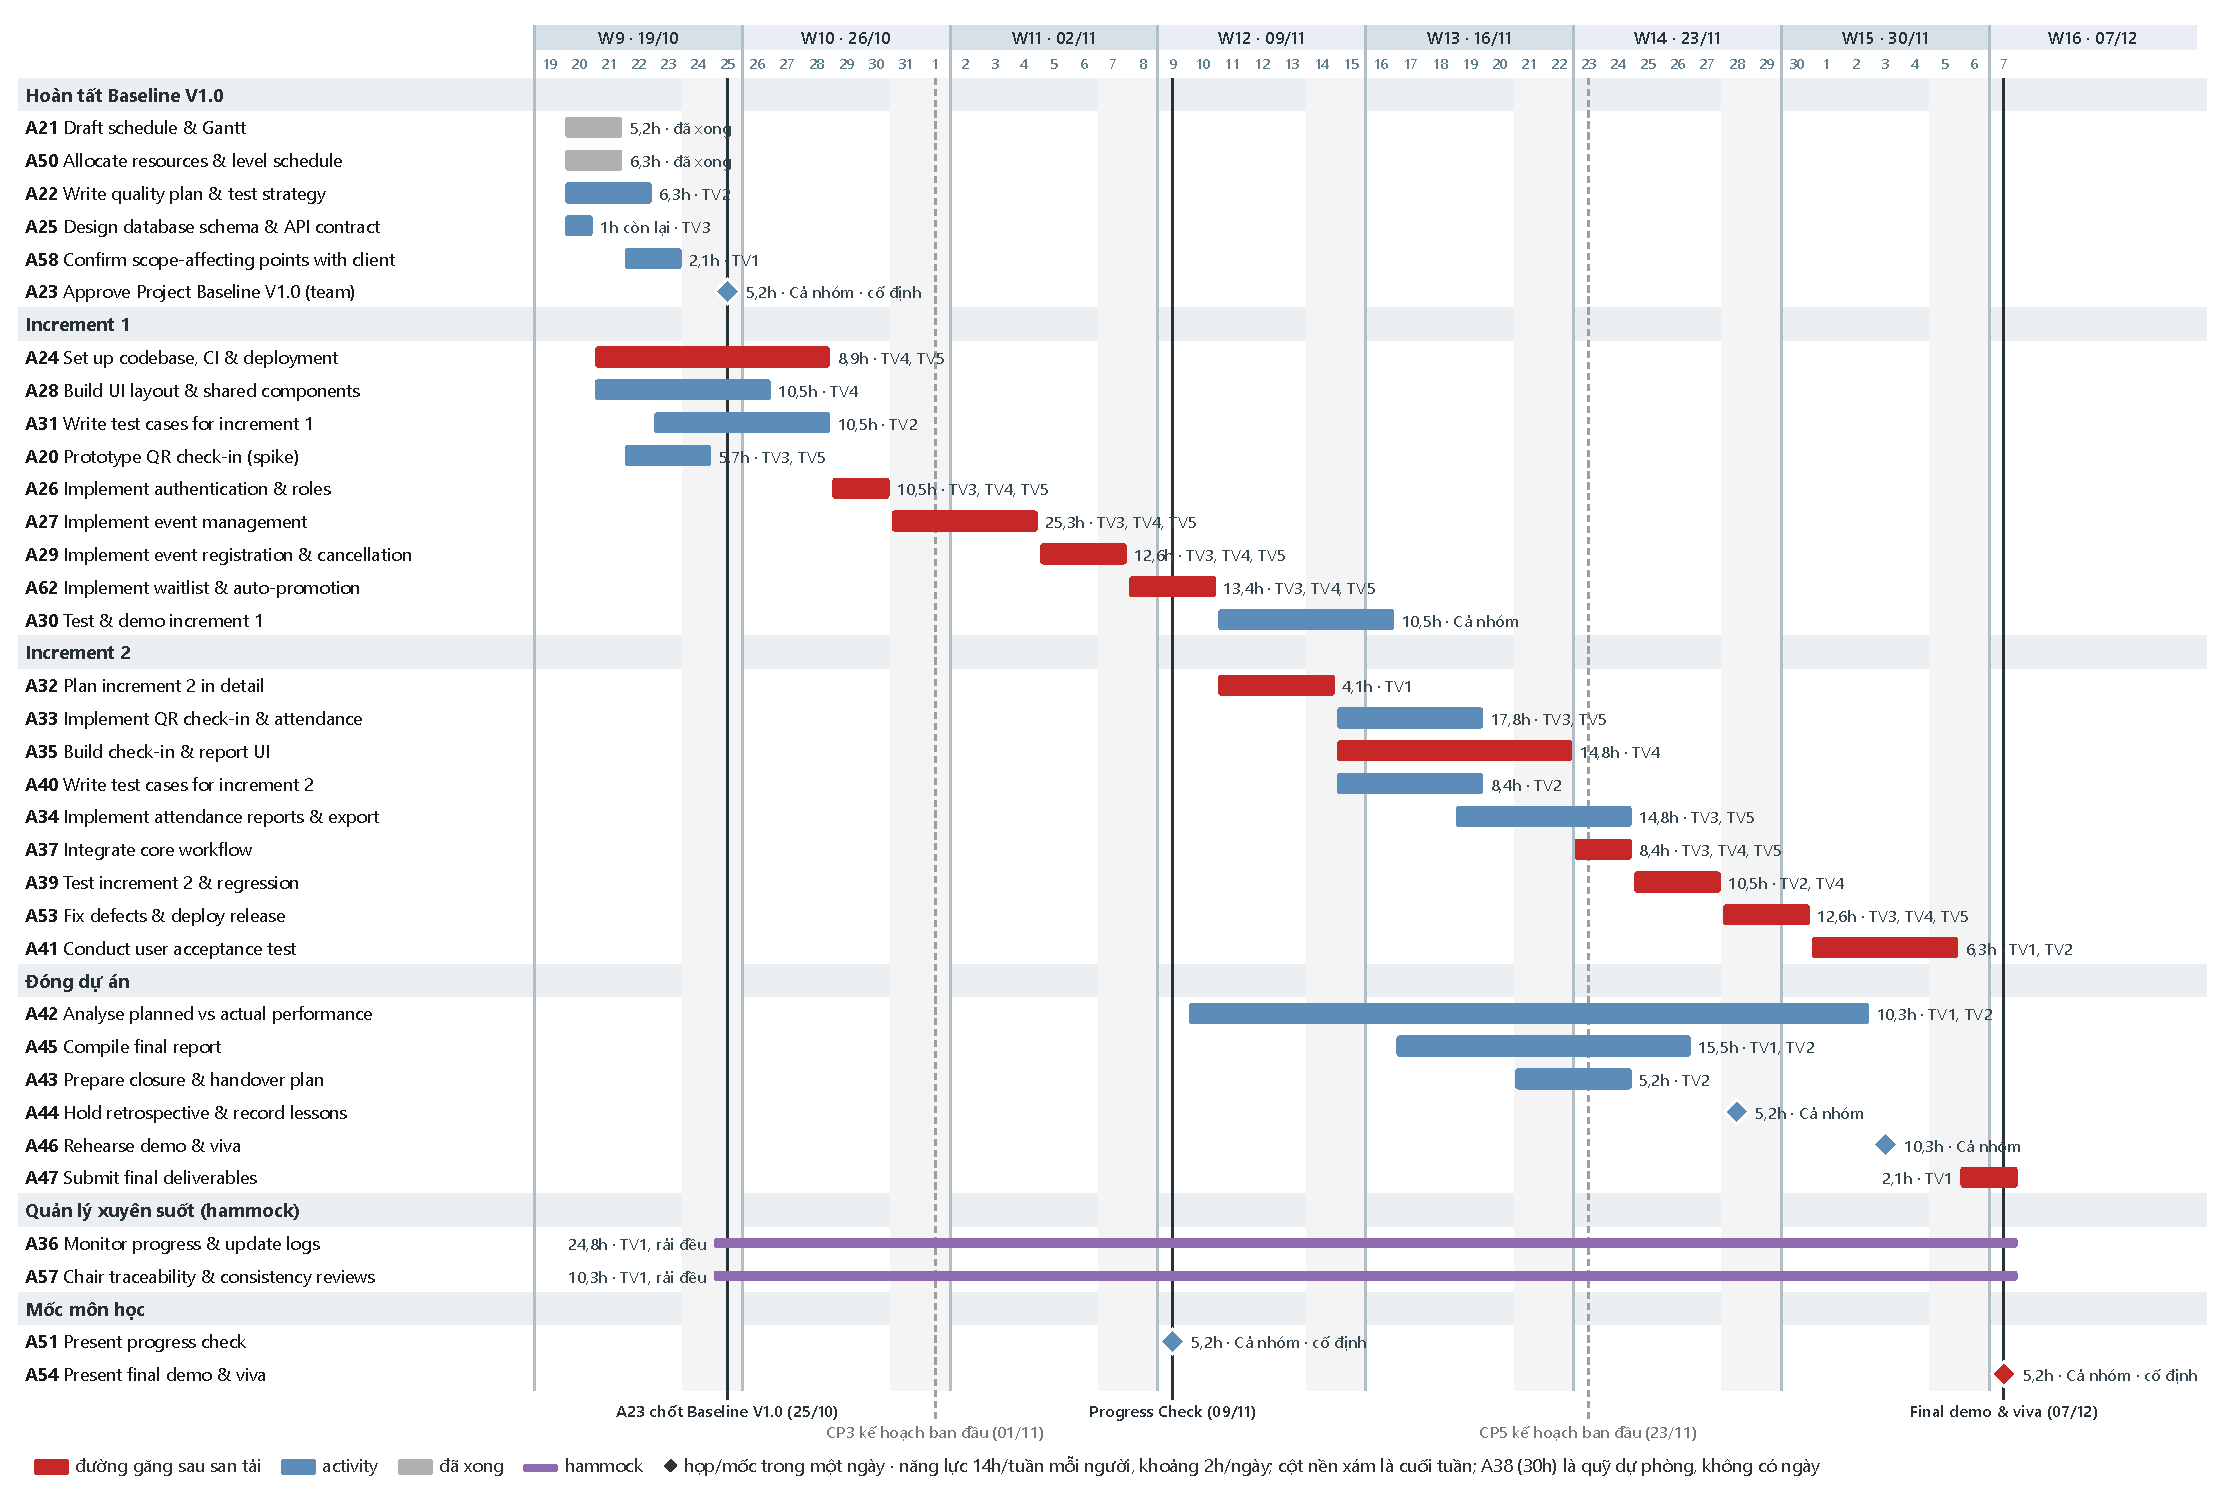
\includegraphics[width=\linewidth,height=0.88\textheight,keepaspectratio]{image/gantt.pdf}
\caption{Gantt Baseline V1.0 (đã san tải, 14 giờ/tuần mỗi người, A23 họp 25/10); thanh đỏ là đường găng}
\label{fig:gantt}
\end{figure}
\end{landscape}

\textbf{Cost baseline.} Đơn vị là giờ người, không quy đổi VND (E04). Các activity làm trước khi ước lượng (A01--A15, A49, A55, A59, A61) không có số ước lượng, chỉ ghi giờ thực tế ở tab Time Tracking (đang thu theo I02).

\begingroup\tblsetup\tblzebra
\begin{longtable}{L{4.6cm}L{7.4cm}>{\raggedleft\arraybackslash}p{2.2cm}}
\caption{Cost baseline theo giai đoạn (giờ người)}\label{tab:cost-baseline}\\
\toprule
\rowcolor{tblheadbg}\textbf{Giai đoạn} & \textbf{Activity} & \textbf{Effort} \\
\midrule
\endfirsthead
\toprule
\rowcolor{tblheadbg}\textbf{Giai đoạn} & \textbf{Activity} & \textbf{Effort} \\
\midrule
\endhead
\bottomrule
\endlastfoot
Lập kế hoạch Task 2 & A16, A17, A18, A19, A22, A25, A21, A20, A50, A58, A23 & 70,2 \\
Increment 1 & A24, A26, A28, A31, A27, A29, A62, A30 & 102,2 \\
Increment 2 và kiểm thử & A32, A33, A34, A35, A40, A37, A51, A39, A53, A41 & 102,9 \\
Đóng dự án & A42, A43, A44, A45, A46, A47, A54 & 53,8 \\
Quản lý xuyên suốt & A36, A57 & 35,1 \\
\textbf{Cộng effort kế hoạch} &  & \textbf{364,2} \\
Quỹ dự phòng A38 (change event, tách riêng) & A38 & 30,0 \\
\textbf{Cost baseline} &  & \textbf{394,2} \\
\end{longtable}
\endgroup

Quỹ A38 nằm trong giờ dư của TV2--TV5 (mục~\ref{sec:2-10}), nhưng lịch không còn ngày dự trữ: nếu change event rơi vào chuỗi găng thì nhóm cắt Could rồi Should hoặc lập Baseline V2.0. Rủi ro trễ lịch được theo dõi ở R15 (TV1 cập nhật R15 và Risk History ngày 21/10).

\kiemtra{Lịch, Gantt và cost baseline do AI hỗ trợ tính ngày 20/10, chạy lại 21/10 khi TV1 chốt A23 ngày 25/10 (\texttt{tools/schedule/baseline-v1-a23-25-10.json}); TV1 chọn phương án, nhóm xác nhận tại A23 ngày 25/10 (chọn V0). Bản chi tiết: \texttt{docs/task2/2.11-schedule.md}.}

\section{Baseline V1.0}
\label{sec:2-12}
Baseline V1.0 là mốc nội bộ của nhóm (CP2), không phải milestone của môn học (Q16); client không duyệt toàn bộ baseline (P05). Nội dung gồm:
\begin{itemize}
  \item \textbf{Phạm vi:} toàn bộ yêu cầu Must (mục~\ref{sec:1-4}); Should và Could chỉ làm khi còn thời gian, cắt theo thứ tự Could rồi Should, không bỏ core workflow.
  \item \textbf{Sản phẩm và activity:} PBS, PD-01 đến PD-05, PFD và mạng activity (mục~\ref{sec:2-1}--\ref{sec:2-4}, gồm L1--L11).
  \item \textbf{Ước lượng và chi phí:} 364,2 giờ người effort kế hoạch, cộng quỹ dự phòng A38 30 giờ, cost baseline 394,2 giờ người (mục~\ref{sec:2-6}, Bảng~\ref{tab:cost-baseline}).
  \item \textbf{Lịch:} Bảng~\ref{tab:schedule} và Hình~\ref{fig:gantt}; CP3 11--16/11, Progress Check 09/11, UAT 01--05/12, demo 07/12, không còn ngày dự trữ.
  \item \textbf{Tài nguyên:} 14 giờ/tuần mỗi người, phân vai và tải theo tuần ở mục~\ref{sec:2-10}.
  \item \textbf{Rủi ro:} sổ rủi ro cấp activity và activity phản hồi rủi ro (mục~\ref{sec:2-8}, \ref{sec:2-9}); rủi ro lịch chính là R15.
\end{itemize}

Nhóm xác nhận cả 18 mục của checklist A23 tại họp 15h Chủ nhật 25/10/2026 (TV1 báo ngày 27/10), trong đó chọn phương án chia giờ V0 (giữ lịch, không còn ngày dự trữ trước demo 07/12) và giữ GitLab, Jenkins do TV3 giữ. Khoảng đệm bằng không là rủi ro lịch nhóm chấp nhận; nếu A27 trễ quá một ngày thì TV1 xem xét cắt REQ-21 (Should).

\kiemtra{Biên bản chi tiết ở tab Biên bản CP (dòng CP2 bổ sung). Chưa xuất \texttt{v1.0.pdf} và chưa gắn tag \texttt{baseline-v1.0}; khi xong thì đưa bản đầy đủ vào Phụ lục~\ref{app:baselines} và ghi ngày tag.}

\chapter{Thực thi, giám sát và kiểm soát (Task 3)}
\label{chap:task3}

\section{Hiện thực phần mềm}
\label{sec:3-1}
\todo{Tóm tắt các increment đã hiện thực, chức năng đã có, kiến trúc và stack; liên kết tới repo ở Phụ lục~\ref{app:repository}.}

\section{Nhật ký hằng tuần}
\label{sec:3-2}
Weekly log được ghi theo activity trong tab Weekly Log của Sheet master; bảng đầy đủ ở Phụ lục~\ref{app:weekly-logs}. Các điểm đáng chú ý đến tuần 9:
\begin{itemize}
  \item \textbf{W6 (28/09--04/10):} phát hiện Milestone 1 là buổi trình bày 05/10 chứ không phải hạn nộp 11/10 (I01); PM thu hẹp nội dung M1 theo bảng milestone của đề và dời Task~2 sang sau M1.
  \item \textbf{W7 (05--11/10):} ở buổi M1 ngày 05/10 nhóm không được gọi trình bày nên không có nhận xét của client; email vòng 2 gửi 08/10 và được trả lời trong ngày; A16, A17 trễ so với lịch, A19, A22, A25 chưa bắt đầu.
  \item \textbf{W8 (12--18/10):} TV2 duyệt mạng hoạt động và checkpoint, năm PD được duyệt ngày 14/10; CP2 lùi từ 16/10 sang 18/10 và đạt có điều kiện; nhóm chốt stack React, Go, PostgreSQL và phân vai mới.
  \item \textbf{W9 (19--25/10):} phát hiện chưa ai log work trên Jira từ đầu dự án (I02); đồng bộ Jira theo lịch Baseline V1.0 nháp (21/10); phát hiện các thành viên không truy cập được GitLab tự host trên máy cá nhân (I03, 22/10).
\end{itemize}
Cột effort thực tế trong weekly log còn trống cho đến khi thu xong giờ hồi tưởng (hạn 23/10, xem I02).

\todo{Tóm tắt các tuần từ W9 trở đi khi có số liệu.}

\section{So sánh kế hoạch và thực tế}
\label{sec:3-3}
\todo{So sánh effort và lịch planned vs actual theo activity/tuần, phân tích độ lệch và nguyên nhân.}

\section{Cập nhật rủi ro và vấn đề}
\label{sec:3-4}
\subsection*{Issue}
Issue là sự việc đã xảy ra, khác với rủi ro là sự việc có thể xảy ra. Bảng~\ref{tab:issues} lấy từ issue log của nhóm; người xử lý cả ba issue là TV1, chưa issue nào được đóng.

\begingroup\tblsetup\tblzebra
\begin{longtable}{L{0.7cm}L{2.0cm}L{3.2cm}L{2.5cm}L{4.4cm}L{1.0cm}}
\caption{Issue log}\label{tab:issues}\\
\toprule
\rowcolor{tblheadbg}\textbf{ID} & \textbf{Ngày} & \textbf{Mô tả} & \textbf{Ảnh hưởng} & \textbf{Hành động} & \textbf{Rủi ro} \\
\midrule
\endfirsthead
\toprule
\rowcolor{tblheadbg}\textbf{ID} & \textbf{Ngày} & \textbf{Mô tả} & \textbf{Ảnh hưởng} & \textbf{Hành động} & \textbf{Rủi ro} \\
\midrule
\endhead
\bottomrule
\endlastfoot
I01 & 02/10/2026 & Milestone 1 là buổi trình bày trên lớp thứ Hai 05/10, không phải hạn nộp 11/10 như nhóm đã hiểu; thời gian còn lại giảm từ 9 ngày xuống 3 ngày & Chuỗi Task~1 đến M1; A15--A22 & Thu hẹp M1 theo bảng milestone của đề (chỉ Initiation \& Definition, ước lượng effort để sang Task~2); thêm A61, A59; dời Task~2 sang 06--12/10; email vòng 2 chuyển sang sau buổi M1 & R10 \\
I02 & 20/10/2026 & Chưa thành viên nào log work trên Jira từ đầu dự án; tab Time Tracking trống, không có actual effort cho các activity đã làm (A01--A23) & Mục~\ref{sec:3-2}, \ref{sec:3-3}; báo cáo actual effort tại Progress Check 09/11 & Thu giờ hồi tưởng bằng mẫu Time Tracking, mỗi dòng ghi \enquote{ước tính hồi tưởng}, hạn 23/10; từ W9 log work trên Jira khi làm, rà ở họp 15h Chủ nhật & R02, R07 \\
I03 & 22/10/2026 & GitLab của nhóm chạy trên máy cá nhân, các thành viên khác không truy cập được; chưa có repo chung để dựng codebase, review Merge Request, chạy CI và deploy & A24 (găng), A28, A20; stage \texttt{Baseline frozen} & Tạm đến họp 25/10: tài liệu là file \texttt{.md} trên thư mục Drive \texttt{Sprint 6-7}, code dùng git trên máy từng người; CI, deploy, Merge Request dời sang 26--28/10. Họp A23 ngày 25/10 chọn nơi chứa repo và CI; quá 25/10 thì A24 trễ, kéo theo A26 và demo & R11, R15 \\
\end{longtable}
\endgroup

\subsection*{Lịch sử rủi ro}
Bảng~\ref{tab:risk-history} ghi lại các thay đổi của sổ rủi ro tính đến 22/10 (tab Risk History của Sheet master). Các dòng ngày 14/10 được TV1 ghi lại vào ngày 20/10 từ checklist rà soát của TV3.

\begingroup\tblsetup\tblzebra
\begin{longtable}{L{2.0cm}L{0.8cm}L{5.5cm}L{4.3cm}L{1.5cm}}
\caption{Lịch sử thay đổi rủi ro}\label{tab:risk-history}\\
\toprule
\rowcolor{tblheadbg}\textbf{Ngày} & \textbf{ID} & \textbf{Thay đổi} & \textbf{Lý do} & \textbf{Người cập nhật} \\
\midrule
\endfirsthead
\toprule
\rowcolor{tblheadbg}\textbf{Ngày} & \textbf{ID} & \textbf{Thay đổi} & \textbf{Lý do} & \textbf{Người cập nhật} \\
\midrule
\endhead
\bottomrule
\endlastfoot
02/10/2026 & R10 & Rủi ro xảy ra: M1 là buổi trình bày 05/10, không phải hạn nộp 11/10. Chuyển thành issue I01, kích hoạt phương án dự phòng & Nhóm đối chiếu lại thông báo trên lớp & TV1 \\
08/10/2026 & R13 & Đóng: thầy xác nhận không có Milestone 2 và 3, chỉ một Progress Check & Phản hồi Q16 ngày 08/10 (19:58) & TV1 \\
08/10/2026 & R01 & P 3$\rightarrow$2, exposure 12$\rightarrow$8 & Vòng 2 gửi 16:39 được trả lời trong cùng ngày 19:58 & TV1 \\
08/10/2026 & R05 & Cập nhật giảm thiểu: contingency chung thay cho activity riêng & Q17: change event không báo trước nội dung, không tạo activity riêng & TV1 \\
13/10/2026 & R11 & P 3$\rightarrow$2, exposure 12$\rightarrow$8; thêm mirror công khai & PM chốt mirror công khai ngày 13/10 & TV1 \\
13/10/2026 & R14 & Thêm mới: yêu cầu mới từ Q19 làm tăng effort & Phản hồi 08/10 thêm sửa/hủy sự kiện và thông báo & TV1 \\
13/10/2026 & R15 & Thêm mới: lịch vượt Progress Check và demo theo năng lực E01 & Phân tích tải và đề xuất thời lượng (nháp AI) ngày 12/10 & TV1 \\
13/10/2026 & R16 & Thêm mới: báo cáo tích hợp muộn ở A39 & A34 không còn chặn A37 để giữ Progress Check & TV1 \\
13/10/2026 & R17 & Thêm mới: tranh chấp khi waitlist tự chuyển & Q14, Q15: quy tắc waitlist và đăng ký lại & TV1 \\
13/10/2026 & R18 & Thêm mới: thông báo thất bại hoặc thiếu kênh email & Q14: thông báo lỗi không hoàn tác việc chuyển & TV1 \\
13/10/2026 & R19 & Thêm mới: TV1 quá tải & Tải theo tuần vượt 7h khi tính theo effort đã chốt & TV1 \\
13/10/2026 & R20 & Thêm mới: lộ thông tin xác thực khi mirror công khai & Quyết định mirror công khai; file ghi mật khẩu trong thư mục dự án & TV1 \\
14/10/2026 & R02 & Sửa giảm thiểu (tính cả AI review/test/sửa lỗi; báo PM khi vượt) và dự phòng (cân bằng tài nguyên/reserve hoặc đổi scope) & TV3 rà estimate và rủi ro (checklist 14/10) & TV1 (ghi lại 20/10) \\
14/10/2026 & R14 & Sửa giảm thiểu: tính sửa/hủy sự kiện và thông báo trong A27, tránh tính trùng A29; dự phòng: PM/BA xác nhận REQ-21 trước khi cắt & TV3 rà estimate A27, A29 (checklist 14/10) & TV1 (ghi lại 20/10) \\
14/10/2026 & R17 & Sửa giảm thiểu (test FIFO, không chuyển trùng, đồng thời 100 lượt) và dự phòng (fallback thủ công có quyền riêng) & TV3 rà thiết kế waitlist (checklist 14/10) & TV1 (ghi lại 20/10) \\
14/10/2026 & R21 & Thêm mới: giao diện quét QR hoặc form vỡ layout trên điện thoại nhỏ (P3, I4) & Owner TV4 bổ sung, xác nhận 14/10 & TV1 (ghi lại 20/10) \\
14/10/2026 & R22 & Thêm mới: chậm review tài liệu chéo do thành viên bận (P4, I3) & Owner TV4 bổ sung, xác nhận 14/10 & TV1 (ghi lại 20/10) \\
20/10/2026 & R02 & Bổ sung: ý kiến trái chiều về estimate implement/testing tại CP2 18/10; PM giữ số 20/10 & Kết quả CP2 18/10 & TV1 (ghi lại 20/10) \\
20/10/2026 & R19 & Cập nhật giảm thiểu: TV1 nhận toàn bộ phần quản trị và báo cáo từ 18/10; chờ chấm lại P, I & Phân vai lại tại họp 18/10 & TV1 (ghi lại 20/10) \\
22/10/2026 & R15 & Sửa mô tả: năng lực 14h/tuần (E01) thay 12h/tuần; thêm kết quả lịch A21: chỉ vừa kịp 07/12, không còn ngày dự trữ, Progress Check 09/11 chưa có QR check-in & E01 chốt 14h/tuần (20/10); lịch A21 chạy lại 21/10 & TV1 (ghi lại 22/10) \\
22/10/2026 & R05 & Sửa giảm thiểu: A38 là quỹ dự phòng 30h ngoài chuỗi (L6 = B), bỏ \enquote{8 ngày sau Progress Check} & L6 = B, nhóm duyệt tại CP2 18/10 & TV1 (ghi lại 22/10) \\
22/10/2026 & R19 & Sửa mô tả: năng lực khoảng 14h/tuần (E01) thay 7h/tuần, khớp báo cáo & Năng lực TV1 chốt 14h/tuần (A50, 20/10) & TV1 (ghi lại 22/10) \\
\end{longtable}
\endgroup

\todo{Cập nhật rủi ro và issue phát sinh trong Increment 1 và 2; chấm lại P, I theo actual effort.}

\section{Bằng chứng chất lượng}
\label{sec:3-5}
\todo{Kết quả test, review, CI/CD, đối chiếu với tiêu chí chất lượng trong Product Descriptions.}

\section{Phản hồi change event}
\label{sec:3-6}
Theo thầy (Q17, 08/10), change event do thầy đưa ra trong quá trình thực hiện dự án và không báo trước nội dung. Nhóm xem đây là một phần của rủi ro, dành contingency trong kế hoạch và không tạo trước activity riêng.

\todo{Mô tả change event thực tế do giảng viên đưa ra, phân tích tác động, change request, quyết định và người duyệt.}

\section{Baseline V2.0}
\label{sec:3-7}
\todo{Những gì thay đổi so với Baseline V1.0 và lý do; giữ nguyên V1.0 ở Phụ lục~\ref{app:baselines}.}

\section{Kế hoạch cấp thấp}
\label{sec:3-8}
\todo{Kế hoạch chi tiết cho từng increment/sprint (công việc, người, thời gian, tiêu chí hoàn thành).}

\chapter{Bàn giao và đánh giá (Task 4)}
\label{chap:task4}

\section{Bàn giao và phân loại phạm vi}
\label{sec:4-1}
\todo{Danh sách sản phẩm bàn giao; phân loại từng hạng mục scope: hoàn thành, hoàn thành một phần, chưa làm, bị loại/đổi (kèm lý do).}

\section{So sánh kế hoạch và thực tế}
\label{sec:4-2}
\todo{So sánh tổng thể Baseline V1.0/V2.0 với thực tế về scope, lịch, effort, chi phí.}

\section{Đánh giá mục tiêu và MoE}
\label{sec:4-3}
\todo{Đánh giá từng objective và MoE; tách rõ \enquote{sản phẩm đã xong} với \enquote{mục tiêu đã đạt}.}

\section{Kế hoạch đóng dự án}
\label{sec:4-4}
\todo{Các việc đóng dự án: bàn giao tài liệu/mã nguồn, lưu trữ, thu hồi quyền truy cập, xác nhận của client.}

\section{Bài học kinh nghiệm}
\label{sec:4-5}
\todo{Bài học rút ra về ước lượng, rủi ro, giao tiếp, công cụ; mỗi bài học gắn với sự kiện cụ thể trong dự án.}

\section{Đóng góp và reflection cá nhân}
\label{sec:4-6}
\todo{Tóm tắt đóng góp từng thành viên (chi tiết ở Phụ lục~\ref{app:contributions}) và phần reflection cá nhân do chính mỗi người viết.}

\chapter{Ma trận truy vết}
\label{chap:traceability}

Mỗi dòng nối một chuỗi Objective $\rightarrow$ Requirement/Product $\rightarrow$ Activity $\rightarrow$ Resource $\rightarrow$ Risk $\rightarrow$ Test $\rightarrow$ Checkpoint bằng mã định danh. Mã objective theo Bảng~\ref{tab:objectives}, mã yêu cầu theo Bảng~\ref{tab:moscow}, mã sản phẩm S theo PBS (mục~\ref{sec:2-1}), activity theo mạng hoạt động (mục~\ref{sec:2-4}), rủi ro theo Bảng~\ref{tab:risk-high} và~\ref{tab:risk-activity}, checkpoint theo Bảng~\ref{tab:checkpoints}. Ma trận lấy từ tab Traceability của Sheet master (bản export 22/10); cột người duyệt là thành viên xác nhận dòng đó.

\kiemtra{Bốn dòng (O4 và S42) còn chờ duyệt; cột ngày duyệt trong Sheet còn trống. Mã test (T-\ldots) là đề xuất, chốt ở A22. Cột Resource đã đối chiếu với owner ở tab Activity ngày 20/10.}

\begin{landscape}
\begingroup\tblsetup\tblzebra
\begin{longtable}{L{3.0cm}L{4.0cm}L{1.5cm}L{1.7cm}L{1.3cm}L{4.3cm}L{1.3cm}L{1.3cm}}
\caption{Ma trận truy vết}\label{tab:traceability}\\
\toprule
\rowcolor{tblheadbg}\textbf{Objective} & \textbf{Requirement / Product} & \textbf{Activity} & \textbf{Resource} & \textbf{Risk} & \textbf{Test} & \textbf{Check\-point} & \textbf{Người duyệt} \\
\midrule
\endfirsthead
\toprule
\rowcolor{tblheadbg}\textbf{Objective} & \textbf{Requirement / Product} & \textbf{Activity} & \textbf{Resource} & \textbf{Risk} & \textbf{Test} & \textbf{Check\-point} & \textbf{Người duyệt} \\
\midrule
\endhead
\bottomrule
\endlastfoot
O1 Duy trì chính xác đăng ký, số chỗ, waitlist & REQ-05, REQ-06 Capacity, đăng ký và hủy (S33) & A29 & TV3, TV4, TV5 & R17 & T-REG-01 đến 05: không trùng, không vượt chỗ, hủy đến 24 giờ trước giờ bắt đầu sự kiện & CP3 & TV3 \\
O1 & REQ-07, REQ-08, REQ-09 Waitlist, tự chuyển FIFO, thông báo (S33) & A62 & TV3, TV4, TV5 & R17, R18 & T-WL-01 đến 04: FIFO, thông báo lỗi vẫn đăng ký, đăng ký lại & CP3 & TV3 \\
O1 & REQ-03 Tạo và chỉnh sửa sự kiện (S32) & A27 & TV3, TV4, TV5 & R14 & T-EV-01 đến 05 & CP3 & TV3 \\
O1 & REQ-21 Sửa hoặc hủy sự kiện đã công bố (S32), Should & A27, A29 & TV3, TV4, TV5 & R14 & T-EV-06 đến 07: thông báo khi đổi thời gian/địa điểm; hủy sự kiện thì hủy đăng ký, đóng waitlist và thông báo người liên quan & CP3 & TV3 \\
O2 Tăng tốc điểm danh, có phương án dự phòng & REQ-10 Điểm danh bằng QR (S34) & A20, A33 & TV3, TV5, TV2 & R04 & T-CI-01 đến 03: quét, trùng, median $\le$ 5 giây & CP5 & TV5 \\
O2 & REQ-11 Nhập mã hoặc xác nhận thủ công (S34) & A33 & TV5, TV3, TV2 & R04 & T-CI-04 đến 05: cập nhật giống QR & CP5 & TV5 \\
O2 & REQ-10 Giao diện điểm danh mobile-first (S36) & A35 & TV4 & R04, R21 & T-UI-01 & CP5 & TV5 \\
O3 Giảm thời gian lấy thông tin tham dự & REQ-12, REQ-13 Danh sách đăng ký, tham dự, thống kê (S35) & A34 & TV3, TV5 & R16 & T-RP-01 đến 02: số liệu khớp dữ liệu nguồn & CP5 & TV3 \\
O3 & REQ-14 Xuất CSV (mở được bằng Excel) (S35) & A34 & TV3, TV5 & R16 & T-RP-03: 500 lượt đăng ký trong 30 giây & CP5 & TV3 \\
O4 Chỉ vai trò có thẩm quyền mới publish và truy cập & REQ-01, REQ-02 Đăng nhập mô phỏng, phân quyền (S31) & A26 & TV3, TV5, TV4 & R20 & T-AUTH-01 đến 03 & CP3 & chờ duyệt \\
O4 & REQ-04 Duyệt trước khi công bố; Organizer không tự duyệt (S31, S32) & A26, A27 & TV3, TV5, TV4 & R14 & T-AUTH-04: không publish khi chưa duyệt; Organizer không được tự duyệt sự kiện mình tạo & CP3 & chờ duyệt \\
O4 & REQ-15 Bảo vệ dữ liệu cá nhân; quyền xem dữ liệu theo vai trò (Q20) & A26 & TV3, TV5, TV4 & R20 & T-AUTH-05 đến 06 & CP5 & chờ duyệt \\
O1 đến O4 & S42 Tested Integrated System & A37, A39, A53 & TV3, TV4, TV5, TV2 & R15, R16 & T-INT-01 đến 03: luồng end-to-end & CP4, CP5 & chờ duyệt \\
O1 đến O4 & S51 Deployed System & A24, A53, A41 & TV5, TV3, TV4, TV2, TV1 & R09, R11, R20 & T-DEP-01; UAT theo tiêu chí acceptance & CP5 & TV5 \\
Quản lý: Baseline V1.0 nhất quán & M2 Project Baseline & A17 đến A23 & TV1, TV2, TV3, TV4, TV5 & R08, R15 & Review chéo theo checklist CP2 & CP2 & TV1 \\
\end{longtable}
\endgroup
\end{landscape}


% ===================== TÀI LIỆU THAM KHẢO =====================
\renewcommand*\bibname{Tài liệu tham khảo}
\clearpage\phantomsection
\addcontentsline{toc}{chapter}{\bibname}
\begin{thebibliography}{9}
\bibitem{hughes-spm}
B.~Hughes, M.~Cotterell, R.~Mall, \textit{Software Project Management}. McGraw-Hill, \todo{năm và ấn bản đang dùng}.
\end{thebibliography}

% ===================== PHỤ LỤC =====================
\appendix
\chapter{Client Interaction Log}
\label{app:client-log}

Cột Ngày ghi thời điểm client trả lời. Email vòng 2 (08/10) gồm 10 câu: Q10--Q17, Q19, Q20.

\kiemtra{Các dòng ngày 08/10 lấy từ file \texttt{Phản hồi 8\_10.txt}; gửi lúc 16:39 bởi Nguyễn Đức Nghĩa, thầy trả lời lúc 19:58 (do PM cung cấp). Ảnh bằng chứng \texttt{Q10-Q20-2026-10-08-email-tra-loi.png} lưu trên Drive của nhóm (Phụ lục~\ref{app:repository}). Cột \enquote{Tác động} của vòng này do AI đề xuất, TV2 rà lại.}

\kiemtra{Email vòng 2 (08/10) mở đầu bằng câu cảm ơn thầy \enquote{đã nhận xét nhóm ở buổi Milestone 1}. Theo biên bản CP (tab Biên bản CP, dòng M1), buổi 05/10 thầy không gọi nhóm 9 trình bày nên không có nhận xét M1; câu mở đầu trên là nguyên văn email đã gửi, không phải bằng chứng có nhận xét M1 của thầy. TV1 xác nhận cách ghi chú này.}

\kiemtra{Dòng Q21, Q22: câu hỏi theo email TV1 gửi 23/10 15:10, trả lời theo ảnh chụp email TV1 cung cấp 27/10; TV1 lưu ảnh lên Drive (\texttt{Q21-Q22-2026-10-25-email-tra-loi.png}) và dán hai dòng này vào tab Client Log.}

\todo{Bổ sung các vòng trao đổi tiếp theo (trao đổi tại Progress Check 09/11; change event).}

\begingroup\tblsetup\tblzebra
\begin{longtable}{L{2.0cm}L{3.4cm}L{4.8cm}L{3.8cm}}
\caption{Client Interaction Log}\label{tab:client-log}\\
\toprule
\rowcolor{tblheadbg}\textbf{Ngày} & \textbf{Câu hỏi của nhóm} & \textbf{Trả lời của client} & \textbf{Tác động tới dự án} \\
\midrule
\endfirsthead
\toprule
\rowcolor{tblheadbg}\textbf{Ngày} & \textbf{Câu hỏi của nhóm} & \textbf{Trả lời của client} & \textbf{Tác động tới dự án} \\
\midrule
\endhead
\bottomrule
\endlastfoot
24/09/2026 07:48 & \textbf{P01.} Ai đóng vai client/sponsor? Ai duyệt scope và thay đổi? & Trong phạm vi BTL, thầy đóng vai client. Nội dung cần làm rõ về scope, priority hoặc thay đổi yêu cầu thì trao đổi trực tiếp với thầy. & Project authority: người quyết định scope, mức ưu tiên và thay đổi yêu cầu là thầy Nguyễn Minh Tâm. \\
24/09/2026 07:48 & \textbf{P02.} Liên hệ client qua kênh nào? Giới hạn và thời gian phản hồi? & Trao đổi qua email. Không giới hạn số câu hỏi nhưng nên tổng hợp trước khi gửi, tránh nhiều email lẻ. Không cam kết thời gian phản hồi cố định; nhóm cần chủ động liên hệ sớm. & Mỗi vòng hỏi gom câu hỏi vào một email. Vòng 2 hỏi qua email sau buổi Milestone 1. \\
24/09/2026 07:48 & \textbf{P03.} Có nên khảo sát sinh viên thật? Trình bày tách khỏi Client Log? & Không. & Không khảo sát sinh viên. Stakeholder analysis dựa trên trao đổi với client và phân tích của nhóm. \\
24/09/2026 07:48 & \textbf{P04.} Hạn nộp và định dạng Milestone 1? & Đã có thông báo trên lớp. & Theo thông báo trên lớp: Milestone 1 là buổi trình bày trên lớp thứ Hai 05/10/2026. Nhóm phát hiện ngày 02/10 (issue I01). \\
24/09/2026 07:48 & \textbf{P05.} Có liên hệ client trong tuần nghỉ để duyệt baseline không? & Trong tuần nghỉ vẫn liên hệ qua email được. Nhóm không cần chờ client "duyệt" toàn bộ Baseline V1.0; baseline là sản phẩm lập kế hoạch của nhóm dựa trên thông tin, assumptions và constraints đã thu thập. Điểm nào ảnh hưởng đáng kể tới scope hoặc planning thì hỏi trước khi chốt baseline. & Nhóm tự chốt Baseline V1.0. Trước khi chốt, gửi email hỏi thầy các điểm ảnh hưởng đáng kể tới scope hoặc planning. \\
24/09/2026 07:48 & \textbf{P06.} Bằng chứng cho Client Log cần dạng nào? & Không yêu cầu biên bản có chữ ký/xác nhận riêng. Nhóm cần ghi lại được thời điểm trao đổi, câu hỏi, phản hồi của client. & Bằng chứng Client Log là ảnh chụp email; cột Ngày ghi kèm giờ. \\
02/10/2026 19:48 & \textbf{Q08.} Tiêu chí nghiệm thu là gì? Thiếu thời gian thì ưu tiên gì? & Nghiệm thu ưu tiên các workflow cốt lõi: tạo/quản lý sự kiện $\rightarrow$ sinh viên đăng ký/hủy đăng ký $\rightarrow$ quản lý số lượng và danh sách chờ $\rightarrow$ điểm danh $\rightarrow$ xem kết quả/báo cáo. Thông báo/nhắc lịch là chức năng bổ trợ; nếu chưa hoàn thiện đầy đủ thì không ảnh hưởng nhiều bằng các chức năng cốt lõi trên. & Xác định thứ tự ưu tiên scope: 5 workflow cốt lõi là Must; thông báo/nhắc lịch ưu tiên thấp hơn. \\
02/10/2026 19:48 & \textbf{Q03.} Điểm danh làm thế nào? Có check-out? Mạng yếu xử lý ra sao? & Có thể sử dụng QR để điểm danh, đồng thời hỗ trợ nhập mã hoặc xác nhận thủ công làm phương án dự phòng. Không bắt buộc check-out. & Điểm danh bằng QR, có phương án nhập mã hoặc xác nhận thủ công. Check-out ngoài scope. \\
02/10/2026 19:48 & \textbf{Q04.} Giới hạn chỗ, danh sách chờ, hạn chót hủy? & Sự kiện có giới hạn số lượng và có waitlist. Khi có chỗ trống, hệ thống tự động chuyển người đầu tiên trong waitlist sang danh sách đăng ký và gửi thông báo, không cần BTC duyệt lại. Nhóm có thể đề xuất deadline hủy đăng ký phù hợp và ghi rõ giả định. & Giới hạn số chỗ và waitlist tự động (kèm thông báo khi được chuyển lên) là yêu cầu. Nhóm cần tự đặt deadline hủy đăng ký và ghi là assumption. \\
02/10/2026 19:48 & \textbf{Q01.} Ai được tạo sự kiện? Có cần duyệt? & Có thể giả định các đơn vị như Khoa, CLB/Đội/Nhóm và các đơn vị/phòng ban của trường có thể tổ chức sự kiện. Sự kiện cần được người có quyền quản lý/duyệt xác nhận trước khi công bố. Nhóm chủ động đề xuất role cụ thể cho workflow này. & Thêm luồng duyệt sự kiện trước khi công bố. Nhóm cần tự đề xuất các role (đơn vị tổ chức, người duyệt\ldots) và ghi là assumption. \\
02/10/2026 19:48 & \textbf{Q02.} Đăng nhập bằng gì? & Có thể giả định sử dụng tài khoản trường. Không yêu cầu tích hợp SSO thực tế; nhóm có thể mô phỏng bằng email trường hoặc dữ liệu tài khoản mẫu. & Tích hợp SSO thật ngoài scope; đăng nhập bằng tài khoản trường mô phỏng (email trường hoặc tài khoản mẫu). \\
02/10/2026 19:48 & \textbf{Q05.} Báo cáo sau sự kiện gồm gì, định dạng nào? & Báo cáo cơ bản gồm danh sách đăng ký, danh sách tham dự/điểm danh và thống kê số lượng người tham gia. Có thể hỗ trợ xuất Excel/CSV. Không yêu cầu tích hợp trực tiếp với hệ thống điểm rèn luyện trong phạm vi hiện tại. & Phạm vi báo cáo: danh sách đăng ký, danh sách điểm danh, thống kê số người; xuất Excel/CSV. Tích hợp điểm rèn luyện ngoài scope. \\
02/10/2026 19:48 & \textbf{Q06.} Quy mô: sự kiện/tháng, người/sự kiện, check-in đồng thời? & Hiện không có số liệu thực tế về số sự kiện/tháng, số người tham gia hoặc tải đồng thời. Nhóm có thể đưa ra giả định hợp lý để phục vụ thiết kế và kiểm thử, nhưng cần ghi rõ là assumption. & Không có số liệu quy mô. Nhóm cần tự đặt giả định (số sự kiện/tháng, số người/sự kiện, tải check-in đồng thời) và ghi là assumption. \\
02/10/2026 19:48 & \textbf{Q09.} Ràng buộc dữ liệu cá nhân, hosting, nền tảng? & Cần có phân quyền và bảo vệ thông tin cá nhân cơ bản của sinh viên. Không có ràng buộc cụ thể về hosting/nền tảng. Web responsive là đủ, không bắt buộc native mobile app. & Phân quyền và bảo vệ thông tin cá nhân cơ bản là yêu cầu. Không ràng buộc hosting. Web responsive; native app ngoài scope. \\
02/10/2026 19:48 & \textbf{Q07.} Hiện dùng công cụ gì? Tổng hợp mất bao lâu? & Có thể giả định quy trình hiện tại sử dụng các công cụ như form/bảng tính và có một số bước tổng hợp thủ công. & Quy trình hiện tại (giả định theo client): form/bảng tính, tổng hợp thủ công. Nhóm cần tự đặt mốc định lượng nếu dùng cho MoE và business case, ghi là assumption. \\
08/10/2026 19:58 & \textbf{Q10.} Phạm vi. Nhóm hiểu phạm vi cốt lõi gồm: tạo/chỉnh sửa sự kiện $\rightarrow$ duyệt trước khi công bố $\rightarrow$ đăng ký/hủy $\rightarrow$ giới hạn chỗ + waitlist + tự động chuyển người đầu waitlist $\rightarrow$ QR check-in (có nhập mã/xác nhận thủ công dự phòng) $\rightarrow$ báo cáo và xuất Excel/CSV. Nhóm không làm: check-out bắt buộc, SSO thật của trường, ứng dụng native Android/iOS, tích hợp điểm rèn luyện, đồng bộ offline đầy đủ. Thầy xác nhận cách hiểu này đã đúng chưa ạ? & Đồng ý & Chốt scope và exclusions làm đầu vào PBS, Product Description và Baseline V1.0. \\
08/10/2026 19:58 & \textbf{Q11.} Mục tiêu và thước đo thành công. Nhóm đang đặt 4 mục tiêu sau: Không cho đăng ký trùng hoặc vượt số chỗ; waitlist chuyển người theo đúng thứ tự vào trước ra trước. Thời gian check-in trung vị $\leq$ 5 giây trong môi trường test của nhóm; có phương án thủ công khi QR không dùng được; chặn check-in trùng. Với 500 lượt đăng ký, tổng hợp điểm danh và xuất Excel/CSV trong $\leq$ 30 giây, số liệu khớp dữ liệu nguồn. Mọi kiểm thử phân quyền đều đạt; sự kiện chưa được duyệt thì không công bố được; không còn lỗi nghiêm trọng về quyền riêng tư/kiểm soát truy cập khi nghiệm thu. Các mốc hiện trạng "15 giây/người" (check-in) và "20 phút/sự kiện" (tổng hợp sau sự kiện) chỉ là giả định lập kế hoạch của nhóm, không phải số liệu thật. Thầy có đồng ý dùng các mục tiêu này làm tiêu chí thành công của dự án không ạ, hay cần điều chỉnh ngưỡng nào? & Đồng ý & Chốt 4 objective và MoE làm tiêu chí thành công; mốc 15 giây/người và 20 phút/sự kiện vẫn là planning assumption. \\
08/10/2026 19:58 & \textbf{Q12.} Role duyệt sự kiện. Nhóm đề xuất dùng một role riêng là Admin/Approver để duyệt sự kiện trước khi công bố, và Organizer không được tự duyệt sự kiện do mình tạo. Đề xuất này có phù hợp với thầy không ạ? & Mình đồng ý với nguyên tắc Organizer không được tự duyệt sự kiện do mình tạo. Tuy nhiên, trong MVP không cần tách thêm một role độc lập nếu không cần thiết. Có thể sử dụng role Admin/System Administrator để thực hiện chức năng duyệt. & Admin duyệt, không thêm role riêng; Organizer không được tự duyệt sự kiện của mình. \\
08/10/2026 19:58 & \textbf{Q13.} Hạn hủy đăng ký. Nhóm đề xuất một mốc cố định cho toàn hệ thống: sinh viên được tự hủy đăng ký đến 24 giờ trước giờ bắt đầu sự kiện. Sau mốc này hệ thống không cho sinh viên tự hủy, nếu có lý do chính đáng thì sinh viên liên hệ Organizer. Thầy thấy cách này có phù hợp không ạ, hay thầy muốn mốc khác hoặc để Organizer cấu hình theo từng sự kiện? & Đồng ý & Hạn hủy cố định 24 giờ trước giờ bắt đầu, toàn hệ thống. \\
08/10/2026 19:58 & \textbf{Q14.} Chuyển người từ waitlist. Khi có chỗ trống, nhóm dự kiến chuyển ngay người đầu waitlist sang danh sách đăng ký rồi gửi thông báo. Nếu gửi thông báo thất bại, người đó vẫn được xem là đã đăng ký chính thức, hay cần thêm trạng thái "chờ xác nhận" ạ? & Khi có chỗ trống: Hệ thống tự động chuyển người đầu tiên trong waitlist vào danh sách đăng ký. Gửi notification cho sinh viên đó. Không cần thêm trạng thái "chờ xác nhận". Nếu notification gửi thất bại, sinh viên vẫn được xem là đã đăng ký chính thức. Notification chỉ là cơ chế thông báo, không phải điều kiện để hoàn tất việc chuyển trạng thái đăng ký. & Tự chuyển người đầu waitlist và gửi notification; thông báo lỗi vẫn tính đã đăng ký; không có trạng thái chờ xác nhận. \\
08/10/2026 19:58 & \textbf{Q15.} Đăng ký trùng. Nhóm dự kiến chặn một sinh viên có nhiều đăng ký còn hiệu lực cho cùng một sự kiện. Nếu sinh viên đã hủy thì có được đăng ký lại không ạ? Nếu sự kiện đã đầy thì người đó vào cuối waitlist có hợp lý không ạ? & Mình đồng ý với nguyên tắc mỗi sinh viên chỉ có một đăng ký còn hiệu lực cho một sự kiện. Nếu sinh viên đã hủy đăng ký thì được phép đăng ký lại, miễn là sự kiện vẫn còn chỗ hoặc còn nhận waitlist. Nếu sự kiện đã đầy thì sinh viên có thể vào cuối waitlist. & Một đăng ký còn hiệu lực/sinh viên/sự kiện; hủy rồi được đăng ký lại, vào cuối waitlist nếu đầy. \\
08/10/2026 19:58 & \textbf{Q19.} Sửa hoặc hủy sự kiện sau khi công bố. Sau khi sự kiện đã được duyệt và công bố, nếu Organizer sửa các thông tin quan trọng (thời gian, địa điểm, số chỗ) thì sự kiện có cần được duyệt lại không ạ? Organizer có được hủy sự kiện đã công bố không; nếu có thì các đăng ký và waitlist hiện có nên xử lý như thế nào? & Organizer được phép chỉnh sửa hoặc hủy sự kiện đã công bố. Trong MVP, không bắt buộc phải xây dựng một quy trình duyệt lại riêng cho mọi thay đổi. Tuy nhiên, với các thay đổi quan trọng như thời gian hoặc địa điểm, hệ thống cần thông báo cho những sinh viên đã đăng ký để họ biết và có thể hủy đăng ký nếu thay đổi không còn phù hợp. Nếu Organizer hủy sự kiện: Sự kiện được chuyển sang trạng thái Cancelled. Các đăng ký hiện tại được hủy theo sự kiện. Waitlist cũng được đóng/hủy. Các sinh viên liên quan nhận notification. & Yêu cầu mới: sửa/hủy sự kiện đã công bố và thông báo người đã đăng ký. Ảnh hưởng A27, A29 và cơ chế notification. \\
08/10/2026 19:58 & \textbf{Q20.} Quyền xem dữ liệu đăng ký và điểm danh. Nhóm dự kiến: Organizer chỉ xem dữ liệu các sự kiện do mình quản lý; Approver/Admin xem được dữ liệu các sự kiện thuộc những đơn vị tổ chức (Khoa, CLB/Đội/Nhóm, phòng ban) mà mình được giao duyệt; sinh viên chỉ xem đăng ký của chính mình. Cách phân quyền này có phù hợp không ạ? & Đồng ý & Phân quyền xem dữ liệu: Organizer xem sự kiện của mình; Admin xem đơn vị được giao; sinh viên xem đăng ký của chính mình. \\
08/10/2026 19:58 & \textbf{Q16.} Milestone 2 và 3. Hiện tại theo như lịch giảng dạy của thầy thì không có 2 nội dung này. Vậy liệu ta có triển khai báo cáo 2 nội dung này không ạ. Nếu có, mong thầy cho nhóm xin ngày dự kiến và đầu ra bắt buộc của Milestone 2 và Milestone 3 được không ạ? Nhóm cần thông tin này để chốt activity network, Gantt và phân bổ nguồn lực. & Không có milestone 2 \& 3, chỉ có 1 lần progress check trên plan & Không có Milestone 2 và 3, chỉ một Progress Check; CP2 là mốc nội bộ của nhóm. \\
08/10/2026 19:58 & \textbf{Q17.} Change event. Mong thầy cho nhóm biết change event dự kiến diễn ra vào khoảng thời gian nào và dưới hình thức nào (yêu cầu mới trên lớp, email hay thay đổi kịch bản) được không ạ? Nhóm có cần dành sẵn dự phòng (reserve) trong Baseline V1.0 cho change event không ạ? & Change Event sẽ được thầy đưa ra trong quá trình thực hiện project theo yêu cầu của môn học; nhóm không cần biết trước nội dung cụ thể. Nhóm nên xem đây là một phần của uncertainty/risk trong project và có thể dành một mức contingency hợp lý trong kế hoạch, nhưng không cần tạo trước một activity cụ thể với tên "Change Event" hoặc giả định trước nội dung thay đổi. & Change event không báo trước, coi là rủi ro và để contingency; không tạo activity tên Change Event. \\
25/10/2026 07:32 & \textbf{Q21.} Phạm vi demo tại Progress Check 09/11. Theo lịch nhóm đã lập sau khi cân đối thời gian của các thành viên, đến ngày 09/11 nhóm sẽ có: đăng nhập và phân quyền theo vai trò; tạo, duyệt và công bố sự kiện; đăng ký và hủy đăng ký theo hạn 24 giờ, có giới hạn số chỗ; waitlist và tự động chuyển người đầu waitlist đang hoàn thiện (dự kiến xong 10/11); bản thử nghiệm quét QR. Điểm danh QR hoàn chỉnh (có nhập mã hoặc xác nhận thủ công dự phòng) dự kiến xong 23--24/11; toàn bộ workflow gồm báo cáo và xuất Excel/CSV được nghiệm thu trong tuần 01--05/12. Tại Progress Check, nhóm cũng sẽ báo cáo actual effort, tiến độ so với kế hoạch và cập nhật risks/issues. Thầy có đồng ý phạm vi trên là đủ cho Progress Check không ạ? Nếu thầy cần thấy điểm danh chạy được tại Progress Check, nhóm sẽ sắp xếp lại thứ tự công việc hoặc cắt bớt yêu cầu mức Should, Could theo thứ tự đã thống nhất (không bỏ workflow cốt lõi), rồi báo lại thầy lịch điều chỉnh. & Mình đồng ý với phạm vi nhóm đề xuất. Tại Progress Check, nhóm chưa bắt buộc phải hoàn thiện toàn bộ workflow, bao gồm QR check-in và báo cáo/Excel/CSV. Tuy nhiên, các chức năng đã hoàn thành cần có bản demo chạy được, không chỉ trình bày giao diện hoặc mô tả thiết kế. Đối với những chức năng đang phát triển, nhóm cần thể hiện rõ tiến độ và kế hoạch hoàn thành. & Giữ lịch, không đổi thứ tự công việc. Tiêu chí CP4: chức năng đã xong phải demo chạy được; chức năng đang làm (waitlist, QR) trình bày tiến độ và kế hoạch hoàn thành. REQ-10, REQ-11 kiểm ở CP5. \\
25/10/2026 07:32 & \textbf{Q22.} Kênh thông báo tối thiểu. Theo trả lời Q14 và Q19 của thầy, hệ thống phải thông báo cho sinh viên khi được chuyển từ waitlist sang danh sách đăng ký, và khi sự kiện đổi thời gian, địa điểm hoặc bị hủy. Nhóm đề xuất thông báo trong ứng dụng là mức bắt buộc của MVP; gửi email là mức Should, chỉ làm nếu còn thời gian. Đề xuất này có phù hợp với thầy không ạ? & Mình đồng ý với đề xuất của nhóm. & Thông báo trong ứng dụng là Must, email là Should (REQ-09, REQ-21); đóng giả định còn mở về kênh thông báo. \\
\end{longtable}
\endgroup

\chapter{Nhật ký hằng tuần}
\label{app:weekly-logs}

Bảng lấy từ tab Weekly Log của Sheet master (bản export 22/10). Effort kế hoạch của W7--W8 là số kế hoạch nháp tại thời điểm lập lịch tuần.

\todo{Cột Effort TT còn trống do I02 (chưa log work); điền sau khi thu giờ hồi tưởng (hạn 23/10) và từ W9 theo worklog Jira. Bổ sung các tuần tiếp theo.}

\begin{landscape}
\begingroup\tblsetup\tblzebra
\begin{longtable}{L{1.1cm}L{1.6cm}L{1.6cm}L{2.6cm}L{2.6cm}L{1.2cm}L{1.2cm}L{2.6cm}L{2.6cm}L{1.4cm}}
\caption{Nhật ký hằng tuần}\label{tab:weekly-log}\\
\toprule
\rowcolor{tblheadbg}\textbf{Tuần} & \textbf{Từ -- đến} & \textbf{Activity} & \textbf{Công việc kế hoạch} & \textbf{Công việc thực tế} & \textbf{Effort KH (h)} & \textbf{Effort TT (h)} & \textbf{Issues / risks} & \textbf{Hành động quản lý} & \textbf{Người cập nhật} \\
\midrule
\endfirsthead
\toprule
\rowcolor{tblheadbg}\textbf{Tuần} & \textbf{Từ -- đến} & \textbf{Activity} & \textbf{Công việc kế hoạch} & \textbf{Công việc thực tế} & \textbf{Effort KH (h)} & \textbf{Effort TT (h)} & \textbf{Issues / risks} & \textbf{Hành động quản lý} & \textbf{Người cập nhật} \\
\midrule
\endhead
\bottomrule
\endlastfoot
W5 & 21/09 -- 27/09 & A01 & Setup GitLab, Jenkins, Jira, Sheet master & Đã dựng GitLab server, Jenkins, Jira & --- &  &  &  & TV3 \\
W5 & 21/09 -- 27/09 & A02 & Phân tích brief & Phân tích brief & --- &  &  &  & Cả nhóm \\
W5 & 21/09 -- 27/09 & A55 & Gửi email P01–P06 cho giảng viên & Đã gửi và nhận phản hồi & --- &  &  &  & TV1 \\
W5 & 21/09 -- 27/09 & A03 & Soạn câu hỏi vòng 1 & Xong, có phân tích tác động và follow-up & --- &  &  &  & TV4 \\
W6 & 28/09 -- 04/10 & A04 & Hỏi client vòng 1 (2/10) & Đã hỏi & --- &  & I01: Milestone 1 là buổi trình bày 05/10, không phải hạn nộp 11/10 (R10 xảy ra) & 02/10: (1) Milestone 1 bám bảng milestone của đề – Initiation \& Definition (client consultation, evaluation, objectives, stakeholders, infrastructure, lifecycle); ước lượng effort để sang Milestone 2. Phương án giữ đủ nội dung và dồn giờ làm thêm trong 3 ngày bị loại. (2) Hỏi client vòng 2 qua email sau buổi M1 để gộp nhận xét của thầy. (3) Slide M1 do TV1 làm. (4) Phân công lại việc tuần này để giảm tải cho TV2 và TV4. & TV1 \\
W6 & 28/09 -- 04/10 & A05 & Bối cảnh, giả định, ràng buộc & Đã có tài liệu A05 (Project Context and Constraints) & --- &  &  &  & TV1 \\
W6 & 28/09 -- 04/10 & A06 & Business case & Đã có nội dung business case (báo cáo TV4) & --- &  &  &  & TV1 \\
W6 & 28/09 -- 04/10 & A08 & Project authority & Đã có mục 1.5 Thẩm quyền dự án trong báo cáo & --- &  &  &  & TV1 \\
W6 & 28/09 -- 04/10 & A09 & Stakeholder analysis & Đã có bảng stakeholder (báo cáo TV3, mục 1.6) & --- &  &  &  & TV1 \\
W6 & 28/09 -- 04/10 & A10 & Standards, communication plan & Đã có standards và kế hoạch giao tiếp (báo cáo TV3 và TV4, mục 1.7) & --- &  &  &  & TV1 \\
W6 & 28/09 -- 04/10 & A07 & Scope, objectives, MoE & Đã có tài liệu A07 (Scope, Objectives và MoE) & --- &  &  &  & TV1 \\
W6 & 28/09 -- 04/10 & A13 & Lifecycle & Đã có phân tích đặc điểm dự án và lifecycle (báo cáo TV3, mục 1.8) & --- &  &  &  & TV1 \\
W6 & 28/09 -- 04/10 & A61 & Dựng khung slide Milestone 1 & Đã dựng khung slide M1 & --- &  &  &  & TV1 \\
W6 & 28/09 -- 04/10 & A14 & CP1: review chéo project definition & Chưa có biên bản CP1; scope và MoE được client đồng ý ngày 08/10 (Q10, Q11) & --- &  &  &  & TV1 \\
W6 & 28/09 -- 04/10 & A59 & Điền slide M1, tập trình bày & Đã điền slide M1 (Slide M1 - Nhóm 9) & --- &  &  &  & TV1 \\
W7 & 05/10 -- 11/10 & A49 & Trình bày Milestone 1 trên lớp (05/10) & Không trình bày: buổi 05/10 thầy chỉ gọi một số nhóm báo cáo, nhóm 9 không được gọi; không có nhận xét của client & 5 &  & Chưa ghi effort thực tế vào Time Tracking & Không có nhận xét M1 để ghi; xác nhận scope và MoE dựa trên email 08/10 (Q10, Q11) & TV1 \\
W7 & 05/10 -- 11/10 & A11 & Soạn câu hỏi vòng 2 (06/10) & Đã soạn bộ câu hỏi Q10–Q18; bổ sung Q19, Q20 & 3 &  & Chưa ghi effort thực tế vào Time Tracking & Gộp thành một email vòng 2 gửi thầy & TV1 \\
W7 & 05/10 -- 11/10 & A12 & Gửi email vòng 2 và theo dõi (07–08/10) & Gửi 08/10 16:39 bởi Đức Nghĩa; thầy trả lời 19:58 & 4 &  & Q16: không có Milestone 2 và 3; Q17: change event không báo trước. Chưa ghi effort thực tế vào Time Tracking & Cập nhật CP2, CP4 và A38 theo Q16, Q17; đưa yêu cầu mới Q19 vào ước lượng & TV1 \\
W7 & 05/10 -- 11/10 & A15 & Dựng PBS và PFD (06–07/10) & Đã có PBS và PFD (\texttt{A15\_\allowbreak PBS\_\allowbreak PFD.md}) & 10 &  & Mã sản phẩm M/S khác mã P1.x trong repo. Chưa ghi effort thực tế vào Time Tracking & Dùng mã M/S cho báo cáo; thống nhất mã trước khi truy vết & TV1 \\
W7 & 05/10 -- 11/10 & A17 & Dựng activity network và checkpoints (08–09/10) & Bản nháp AI hoàn thành 12/10 (mục 2.4, 2.5); chờ TV2 kiểm & 6 &  & Trễ so với lịch 08–09/10; Jira: In Progress & PM chốt L1, L2, L3 ngày 12–13/10; giao TV2 kiểm & TV1 \\
W7 & 05/10 -- 11/10 & A16 & Viết Product Descriptions, ít nhất 5 (09–10/10) & Chưa có PD do nhóm viết; bản nháp AI 5 PD đã soạn 13/10 để nhóm duyệt & 8 &  & Trễ so với lịch 09–10/10; Jira: Backlog & TV2 viết 3 PD, TV4 viết 2 PD hoặc duyệt bản nháp AI & TV1 \\
W7 & 05/10 -- 11/10 & A18 & Ước lượng effort từ dưới lên (10–11/10) & Đã có khung, đề xuất effort và thời lượng (nháp AI); chờ từng thành viên ước lượng & 10 &  & Jira: In Progress; hạn nhóm điền: tối 14/10 & Gửi hướng dẫn A18 cho nhóm; PM chốt E04 là giờ người, không quy VND & TV1 \\
W7 & 05/10 -- 11/10 & A19 & Rủi ro cấp activity và activity phản hồi (10–11/10) & Chưa làm; có đề xuất rủi ro nháp AI trong Risk Register & 8 &  & Jira: Backlog; chờ A17 & TV5 và TV4 chấm P, I và bổ sung rủi ro cấp activity & TV1 \\
W7 & 05/10 -- 11/10 & A22 & Quality plan và chiến lược test (11–12/10) & Chưa làm; chờ A16 & 6 &  & Jira: Backlog & TV2 và TV4 viết quality plan sau khi có PD & TV1 \\
W7 & 05/10 -- 11/10 & A25 & Thiết kế database và API contract (11–13/10) & Chưa làm & 6 &  & Jira: Backlog; cần thêm yêu cầu Q14, Q15, Q19 vào thiết kế & TV3 vẽ ERD, TV4 review API contract & TV1 \\
W8 & 12/10 -- 18/10 & A21 & Lịch, Gantt, critical path (12/10) & Đang làm (Jira: In Progress); chờ A18 và A19; TV3 xác nhận 14/10 A21 chưa bắt đầu & 5 &  & Phụ thuộc A18 và A19 & TV3 tính đường găng khi có số ước lượng của nhóm & TV1 \\
W8 & 12/10 -- 18/10 & A58 & Email các điểm ảnh hưởng scope (13–14/10) & Chưa gửi; bản nháp đã viết lại sau phản hồi 08/10 & 2 &  & Chỉ gửi khi A18 xác nhận lịch vượt hoặc còn câu hỏi & TV1 quyết định có gửi hay không & TV1 \\
W8 & 12/10 -- 18/10 & A20 & Spike check-in QR (13–15/10) & Chưa bắt đầu & 6 &  & Stack kỹ thuật chưa chốt & Chốt stack trước khi làm spike & TV1 \\
W8 & 12/10 -- 18/10 & A50 & Phân bổ tài nguyên, cân bằng lịch (13–15/10) & Chưa bắt đầu; chờ A21 & 6 &  & Tuần nghỉ chỉ khoảng 6h/người (E02) & Thu lịch rảnh và lịch thi của từng người & TV1 \\
W8 & 12/10 -- 18/10 & A23 & Chốt Baseline V1.0 (CP2, 16/10) & Họp CP2 ngày 18/10: đạt có điều kiện; hạn hoàn tất điều kiện 23/10 & 5 &  & CP2 là mốc nội bộ, không phải milestone của môn (Q16) & Review chéo theo checklist CP2 & TV1 \\
W8 & 12/10 -- 18/10 & A24 & Thiết lập codebase, CI và deploy (đến 18/10) & Chưa bắt đầu & 8 &  & Chưa có owner trên Jira; stack chưa chốt & Gán owner (đề xuất TV5) & TV1 \\
W8 & 12/10 -- 18/10 & A23 & Họp định kỳ 18/10 (CP2) & Chốt phân vai (TV1 quản trị và báo cáo; TV2 kiểm thử; TV3, TV5 backend; TV4 frontend); stack React, Go, PostgreSQL; L1–L7; cam kết Must &  &  & Estimate implement/testing còn ý kiến trái chiều; CP2 lùi 16/10 $\rightarrow$ 18/10 (deviation) & PM giữ số estimate (20/10); hạn điều kiện CP2 23/10 & TV1 \\
W8 & 12/10 -- 18/10 & A17 & Rà và duyệt activity network, checkpoints & TV2 duyệt 2.4 v0.7 và 2.5 v0.3 ngày 14/10; PM thêm L7 ngày 15/10; nhóm duyệt L1–L7 tại CP2 18/10 &  &  &  &  & TV1 \\
W8 & 12/10 -- 18/10 & A16 & Duyệt Product Descriptions & 5 PD (AI hỗ trợ soạn) được duyệt 14/10: TV2 PD-01, PD-04, PD-05; TV4 PD-02, PD-03; TV3 PD-02 &  &  &  &  & TV1 \\
W8 & 12/10 -- 18/10 & A18 & Hoàn thành ước lượng (hạn tối 14/10) & TV3 xác nhận estimate 10 activity (phần TV3 khoảng 65,67h) và năng lực 14h/tuần ngày 14/10; thành viên khác chưa ước lượng; CP2 18/10 nhóm đồng ý phần lớn &  &  & Không có vòng ước lượng chéo độc lập; implement/testing còn ý kiến trái chiều & PM giữ số hiện tại 20/10 (A20 P = 6 theo TV3); theo dõi qua R02 & TV1 \\
W8 & 12/10 -- 18/10 & A19 & Rủi ro cấp activity & TV3 duyệt kế hoạch xử lý R02, R06, R14, R16, R17 ngày 14/10; thêm R21, R22 (owner TV4) ngày 14/10 &  &  & Các rủi ro còn lại chưa chấm lại &  & TV1 \\
W8 & 12/10 -- 18/10 & A25 & Thiết kế database và API contract & Chưa bắt đầu tính đến 14/10 (TV3 xác nhận) &  &  & Stack chưa chốt đến 18/10 & Stack chốt 18/10: React, Go, PostgreSQL & TV1 \\
W9 & 19/10 -- 25/10 & A36 & Theo dõi tiến độ, ghi actual effort & 20/10: kiểm tra Jira, chưa ai log work từ đầu dự án; tab Time Tracking trống &  &  & I02: thiếu actual effort cho các activity đã làm (A01–A23) & Gửi mẫu Time Tracking để từng người ghi giờ hồi tưởng; từ W9 log work trên Jira khi làm & TV1 \\
W9 & 19/10 -- 25/10 & A57 & Rà truy vết và nhất quán báo cáo với Sheet & 20/10: điền báo cáo từ Sheet (1.8, 2.2, 2.5, 2.6, 2.8, 2.9, 3.2, 3.4, Chương 5, Phụ lục A, B, D); phát hiện 9 điểm lệch giữa báo cáo và Sheet &  &  & R08: CP3, CP5 ghi khác nhau; Effort tab Activity của A16--A23, A58 chưa theo PERT; cột Resource ở Traceability thiếu owner (7 dòng); cột ước lượng chéo mâu thuẫn báo cáo 2.6 & Sửa báo cáo và 19 ô Sheet ngày 20/10; ngày ES/EF tab Activity chuyển cho A21 & TV1 \\
W9 & 19/10 -- 25/10 & A19 & Duyệt activity phản hồi rủi ro & TV1 duyệt bảng 2.9 (AI hỗ trợ tổng hợp từ Risk Register) ngày 20/10 &  &  & --- & --- & TV1 \\
W9 & 19/10 -- 25/10 & A36 & Đồng bộ Jira theo lịch Baseline V1.0 nháp (A21) & 21/10: import lại 34 task, hoàn thiện A62 (SCRUM-72), đổi tên A38, A53; xóa 34 task cũ trùng mã; export trước/sau ở \texttt{docs/\allowbreak task3/} &  &  & Phát hiện estimate import đợt 03/10 bị chia 60 (A01 hiện 6 phút); importer không đọc 5h 12m & Import bằng số giây $\times$ 60, đã thử trước với task TEST; 23 task đã xong giữ estimate cũ & TV1 \\
W9 & 19/10 -- 25/10 & A24 & Dựng codebase, CI, deploy (21--28/10) & 22/10: nhóm không truy cập được GitLab tự host (máy cá nhân) &  &  & I03: chưa có repo chung cho code, review, CI, deploy & Tạm: tài liệu \texttt{.md} lên Drive, code git local, CI/deploy dời 26--28/10; họp 25/10 chọn nền tảng repo và CI & TV1 \\
W9 & 19/10 -- 25/10 & A21 & Tính CPM, Gantt, cost baseline (20--22/10) & Xong 20--21/10 (TV1 báo); cost baseline 364,2h + A38 30h = 394,2h & 5,2 &  &  & Chạy lại lịch 21/10 khi TV1 chốt A23 ngày 25/10 &  \\
W9 & 19/10 -- 25/10 & A50 & San tải theo năng lực 14h/tuần (23--26/10) & Xong 20--21/10 (TV1 báo); TV2, TV4, TV5 xác nhận phần việc mới (L9) 21/10 & 6,3 &  & R15: lịch vừa kịp 07/12, 0 ngày dự trữ; Progress Check chưa có QR & Cập nhật R15, Risk History 21/10 (TV1 báo); hỏi thầy phạm vi Progress Check (A58) &  \\
W9 & 19/10 -- 25/10 & A22 & Quality plan và test strategy (20--22/10) & Jira 21/10: In Progress & 6,0 &  &  &  &  \\
W9 & 19/10 -- 25/10 & A25 & TV3 xác nhận phần bổ sung PD-02 (20/10) & Jira 21/10: In Review & 1,0 &  &  &  &  \\
W9 & 19/10 -- 25/10 & A24 & Dựng repo, CI, deploy khung (21--28/10) &  & 4,5 &  & CI dùng Jenkins (TV1 chốt 21/10); chưa chọn hosting & TV5 chọn hosting free-tier (ASM-05) &  \\
W9 & 19/10 -- 25/10 & A28 & Layout và component dùng chung (21--26/10) &  & 10,0 &  &  &  &  \\
W9 & 19/10 -- 25/10 & A20 & Spike QR, timebox 6h (22--24/10) &  & 5,7 &  &  &  &  \\
W9 & 19/10 -- 25/10 & A58 & Gửi email hỏi phạm vi Progress Check và kênh notification (22--23/10) & Jira 21/10: In Progress; email v0.3 đã soạn, chưa gửi & 2,1 &  &  & Nếu 24/10 chưa có trả lời thì ghi giả định còn mở tại A23 &  \\
W9 & 19/10 -- 25/10 & A31 & Viết test case Increment 1 (23--28/10) &  & 6,0 &  &  &  &  \\
W9 & 19/10 -- 25/10 & A23 & Họp chốt Baseline V1.0 (25/10, 15h) &  & 5,2 &  &  & Theo checklist \texttt{docs/\allowbreak baseline/\allowbreak A23-checklist.md} &  \\
W10 & 26/10 -- 01/11 & A24 & Hoàn tất repo, CI, deploy khung (đến 28/10) &  & 4,5 &  &  &  &  \\
W10 & 26/10 -- 01/11 & A28 & Hoàn tất layout (26/10) &  & 0,5 &  &  &  &  \\
W10 & 26/10 -- 01/11 & A31 & Hoàn tất test case Increment 1 (đến 28/10) &  & 4,5 &  &  &  &  \\
W10 & 26/10 -- 01/11 & A26 & Đăng nhập, phân quyền (29--30/10) &  & 10,5 &  &  &  &  \\
W10 & 26/10 -- 01/11 & A27 & Quản lý sự kiện, phần đầu (31/10--01/11; kết thúc 04/11) &  & 12,0 &  &  &  &  \\
W10 & 26/10 -- 01/11 & A36 & Theo dõi tiến độ, weekly log; rà log work Jira ở họp 15h Chủ nhật 25/10, 01/11 &  &  &  &  & Từ W9 mỗi Chủ nhật xuất Jira CSV để chuyển thành dòng tab 3 &  \\
\end{longtable}
\endgroup
\end{landscape}

\chapter{Các phiên bản Baseline}
\label{app:baselines}

\section{Baseline V1.0}
Ngày chốt: 25/10/2026 (họp A23, cả nhóm xác nhận, TV1 ký). Nội dung baseline xem mục~\ref{sec:2-12}.

\todo{Bản đầy đủ Baseline V1.0 như lúc chốt (\texttt{v1.0.pdf}, không chỉnh sửa sau đó) và ngày gắn tag \texttt{baseline-v1.0}; điền sau khi xuất PDF.}

\section{Các bản sửa đổi}
\todo{Từng bản sửa đổi (V2.0, \ldots): ngày, change request liên quan, danh sách thay đổi so với bản trước.}

\chapter{Khai báo sử dụng AI}
\label{app:ai-declaration}

\todo{Bổ sung các lần dùng AI tiếp theo; điền cột \enquote{Nhóm đã kiểm tra} cho các dòng còn trống.}

\kiemtra{Bảng lấy từ tab AI Log (bản export 22/10), xếp theo ngày. TV1 điền cột \enquote{Nhóm đã kiểm tra} cho dòng 15/10 và dòng 20/10 (rà Sheet, PD); điền cột \enquote{Người dùng} cho dòng 20/10 (CPM, Jira); bổ sung dòng TV3 dùng AI rà estimate (14/10) và các lần dùng AI từ 05/10 đến 11/10 (A11, A15, A16). Tab AI Log trên Sheet đang thiếu 5 dòng 23/09--02/10 (phụ lục vẫn giữ); dòng 23/10 chờ dán vào Sheet.}

\begingroup\tblsetup\tblzebra
\begin{longtable}{L{2.0cm}L{1.6cm}L{3.0cm}L{3.3cm}L{2.6cm}L{1.3cm}}
\caption{Nhật ký sử dụng AI}\label{tab:ai-log}\\
\toprule
\rowcolor{tblheadbg}\textbf{Ngày} & \textbf{Công cụ} & \textbf{Task / artifact} & \textbf{Dùng để làm gì} & \textbf{Nhóm đã kiểm tra và điều chỉnh} & \textbf{Người dùng} \\
\midrule
\endfirsthead
\toprule
\rowcolor{tblheadbg}\textbf{Ngày} & \textbf{Công cụ} & \textbf{Task / artifact} & \textbf{Dùng để làm gì} & \textbf{Nhóm đã kiểm tra và điều chỉnh} & \textbf{Người dùng} \\
\midrule
\endhead
\bottomrule
\endlastfoot
23/09/2026 & Claude & Kế hoạch tổng thể (\texttt{plan/\allowbreak index.html}) & Lập khung kế hoạch, Gantt, template, chi tiết activity &  & TV1 \\
02/10/2026 & Claude & Cấu trúc \texttt{docs/\allowbreak }, template, cấu hình CI & Dựng khung thư mục và template tài liệu &  & TV1 \\
02/10/2026 & Claude & Sheet master; cập nhật kế hoạch theo P01–P06 và mốc M1 05/10 & Dựng file sheet, cập nhật lịch và tài liệu &  & TV1 \\
02/10/2026 & Claude & Sheet master (file này) & Lọc bỏ dữ liệu Claude đề xuất; chỉ giữ dữ liệu thật, quyết định đã đưa ra và các dòng ví dụ &  & TV1 \\
02/10/2026 & Claude & Kế hoạch HTML, file import Jira, tài liệu trong repo & Lưu ý: số effort, thời lượng, lịch, rủi ro, PD trong các file này là bản nháp Claude đề xuất, không phải số liệu của nhóm; chỉ dùng tham khảo &  & TV1 \\
03/10/2026 & Claude Code & Khung báo cáo LaTeX & Dựng khung báo cáo theo Task 1–4; đưa dữ liệu client và quyết định đã chốt vào báo cáo & Không dùng số liệu nháp AI; sửa người gửi vòng hỏi 1; bỏ nội dung ngoài yêu cầu của đề; bổ sung tên, MSSV thành viên & TV1 \\
04/10/2026 & Claude & Slide M1 - Nhóm 9 & Biên soạn và tổng hợp slide & So sánh với báo cáo & TV1 \\
04/10/2026 & Claude Code & M1-followup-drafts.md & Soạn bản nháp email vòng 2 và tin nhắn nhóm trước M1 & Bản nháp tham khảo, PM sửa trước khi dùng; email vòng 2 thực tế gửi 08/10 16:39 & TV1 \\
04/10/2026 & Claude Code & M1-slide-update-TV4.md và M1-slide-text-updates.md & Đối chiếu báo cáo TV4 với tài liệu nhóm; soạn lại chữ placeholder, slide 4 và 9, nháp business case & PM đối chiếu với TV4: giờ trả lời client là 02/10 19:48; bỏ Vue 3/React vì stack chưa chốt; 585h là capacity, không phải effort; nhắc lịch giữ mức Should & TV1 \\
06/10/2026 & Claude & File tách công việc task 2 cho từng người & Chia nhỏ phân công Task 2 theo từng người, dựa trên trang kế hoạch nháp & So sánh với đề & TV1 \\
12/10/2026 & Claude Code & Task 2: mạng hoạt động, checkpoint, ước lượng, file import Sheet, chương 2 báo cáo & Dựng bản nháp để nhóm duyệt; sinh sơ đồ từ danh sách activity; đề xuất effort và thời lượng; phân tích tải theo tuần & PM chốt E04 là giờ người, L1 theo PFD, hạn A18 tối 14/10; số effort và thời lượng là đề xuất AI, nhóm chốt ở A18, chưa dùng làm số của nhóm & TV1 \\
12/10/2026 & Claude Code & A58-email-xac-nhan-scope.md & Soạn bản nháp email xác nhận các điểm ảnh hưởng scope & Chưa gửi; viết lại sau phản hồi 08/10; PM quyết định có gửi hay không & TV1 \\
13/10/2026 & Claude Code & Báo cáo: cập nhật theo phản hồi 08/10, giả định ASM-02, ASM-06, ASM-07, ghi chú highlight & Đề xuất giá trị giả định theo yêu cầu PM; cập nhật báo cáo; đề xuất xử lý A34 và A38 & PM chốt 13/10: cắt scope Could rồi Should, REQ-21 là Should, mirror công khai, thông báo trong ứng dụng bắt buộc; nhóm rà lại ASM-02, ASM-06, ASM-07 & TV1 \\
13/10/2026 & Claude Code & Nội dung các tab Risk Register, Product Description, Traceability, Biên bản CP, Weekly Log & Soạn nháp để nhóm duyệt và dán vào Sheet & P, I, owner, mã test và nội dung PD là đề xuất AI; TV5, TV2, TV4 duyệt & TV1 \\
15/10/2026 & Claude Code & 2.4 v0.8 (L7), rà 2.4/2.5, danh sách sửa Sheet 15/10 & Đề xuất phương án tách A20 khỏi A24 (L7); rà 2.4, 2.5; liệt kê ô cần sửa theo checklist TV3 &  & TV1 \\
18/10/2026 & Claude Code & Nội dung họp 18/10 (agenda, bản nói CP2) & Soạn agenda và bản nói cho buổi họp chốt Baseline V1.0 & So sánh với hiện tại của báo cáo & TV1 \\
20/10/2026 & Claude Code & Rà Sheet master, PD theo Q01–Q20; cập nhật 2.4, 2.5, 2.6, báo cáo chương 1–2; bản Sheet đã sửa & So sánh Sheet 15/10 và 20/10; đề xuất sửa PD-01, PD-02, PD-03; gỡ nhãn nháp cho nội dung đã duyệt; đề xuất owner theo phân vai 18/10 &  & TV1 \\
20/10/2026 & Claude Code & Báo cáo: mục 1.8, 2.2, 2.5, 2.6, 2.8, 2.9, 3.2, 3.4, Chương 5, Phụ lục A, B, D; rà chéo báo cáo với Sheet & Chuyển dữ liệu Sheet master (export 20/10) vào báo cáo bằng script; tính PERT; tổng hợp bảng activity phản hồi rủi ro (2.9); liệt kê điểm lệch giữa báo cáo và Sheet & TV1 chọn phạm vi và cách xử lý lệch (CP5 \enquote{tuần kế tiếp}, đổi tên cột ước lượng chéo, tự sửa 19 ô trên Google Sheet); AI phát hiện và sửa lỗi làm tròn PERT do chính nó gây ra; TV1 duyệt bảng 2.9 ngày 20/10 & TV1 \\
20/10/2026 & Claude Code & Tính CPM, san tải A21/A50, file import Jira và hướng dẫn & Tính CPM, san tải A21/A50, soạn file import Jira và hướng dẫn & Tự thêm thử task giả nhiều cách để tìm ra nguyên nhân sau đó xóa &  \\
21/10/2026 & Claude Code & 2.6 báo cáo và 2.6-estimates.md (A18) & Tìm nguyên nhân lệch tổng effort 363,7 và 364,2 (làm tròn PERT); sửa tổng, câu mô tả cách cộng, E01, cột thời lượng & TV1 chọn 364,2 + 30 = 394,2 (21/10); chờ nhóm xác nhận tại A23 & TV1 \\
21/10/2026 & Claude Code & tools/schedule (baseline-v1-a23-25-10.json), 2.11 v0.3, 2.10 v0.3, 10-activity-A23-25-10.tsv (A21, A50) & Chạy lại CPM và san tải khi A23 họp 25/10; thêm khóa not\_before vào script (kiểm baseline-v1.json cho kết quả như cũ) & TV1 chốt A23 ngày 25/10; ngày từ A24 trở đi không đổi; chờ nhóm xác nhận tại A23 & TV1 \\
21/10/2026 & Claude Code & 2.5-checkpoints.md v0.5, báo cáo mục 2.5 & Ghi ngày dự kiến CP3, CP5 theo lịch A21 và deviation; đánh dấu CP4 chờ A58 & TV1 duyệt & TV1 \\
21/10/2026 & Claude Code & tools/diagrams, báo cáo mục 2.4, 2.10, 2.11, 2.12 & Vẽ lại 3 hình mạng activity, Gantt bằng HTML/SVG xuất PDF (Chrome headless); đưa lịch, đường găng, cost baseline, san tải vào báo cáo; khung 2.12 & TV1 yêu cầu vẽ bằng HTML thay tikz; chờ nhóm xác nhận tại A23 & TV1 \\
21/10/2026 & Claude Code & Sơ đồ kiến trúc (báo cáo mục 1.7, architecture.html) & Vẽ sơ đồ React $\to$ Go $\to$ PostgreSQL từ PD-01–PD-03, Client Log, checklist TV3 & TV3, TV5 duyệt & TV1 \\
21/10/2026 & Claude Code & docs/task3/increment1-task-specs.md & Soạn mô tả task Increment 1 (A24, A28, A31, A20, A26, A27, A29, A62, A30) theo khung mục tiêu, đầu vào, bước, đầu ra, hoàn thành khi & Endpoint, migration là đề xuất; TV3, TV5, TV4, TV2 đã duyệt phần của mình, TV1 đã duyệt trước khi giao & TV1 \\
21/10/2026 & Claude Code & A58-email-xac-nhan-scope.md v0.3 & Soạn email hỏi phạm vi Progress Check 09/11 và kênh notification tối thiểu & TV1 chọn đề xuất \enquote{trong ứng dụng bắt buộc, email là Should}; TV1 sửa và tự gửi & TV1 \\
21/10/2026 & Claude Code & docs/baseline/A23-checklist.md, 2-weekly-log-W9-W10-ke-hoach.tsv & Soạn checklist họp A23, các mục cần xác nhận, kế hoạch Sprint 7, dòng kế hoạch Weekly Log W9–W10, các bước xuất PDF và gắn tag & TV1 đã duyệt trước họp 25/10 & TV1 \\
22/10/2026 & Claude Code & docs/task3/sprint6-7-viec-theo-nguoi.md, baseline/A23-checklist.md mục 17 & Soạn việc theo từng người Sprint 6–7 từ lịch san tải 2.11 v0.3 (giờ theo ngày); mô tả A22, A25, A58, A23 theo khung; chạy thử phương án chia giờ A26, A24 (V1, V2) trên bản sao script & TV1 chọn giữ lịch V0 (22/10); V1, V2 đưa ra họp A23; TV1 đã duyệt & TV1 \\
22/10/2026 & Claude Code & docs/task3/sprint6-7-viec-theo-nguoi.md v0.2 & Viết lại mô tả chi tiết từng task theo người, không trỏ file khác (chép quy tắc nghiệp vụ, REQ, bộ test case đề xuất, email A58, mục họp A23); bước kỹ thuật, tên bảng, endpoint, thư viện ghi nhãn Đề xuất AI & TV1 yêu cầu 22/10; TV1 duyệt, TV2–TV5 duyệt phần của mình & TV1 \\
22/10/2026 & Claude Code & docs/task3/sprint6-7/ (README, TV1–TV5) v0.3 & Tách giao việc thành 5 file độc lập theo người, có bảng tóm tắt; chép nội dung thay file đính kèm (quality plan v0.2 mẫu, khung test-cases, mô tả sơ đồ kiến trúc, đoạn Jenkins Baseline frozen và Build \& test đề xuất) & TV1 yêu cầu 22/10; TV1 duyệt, TV2–TV5 duyệt phần của mình & TV1 \\
22/10/2026 & Claude Code & Báo cáo mục 1.3, 1.7, 1.8, 2.2, 2.6, 2.8, 2.9, bìa, Phụ lục D; CLAUDE.md; PROGRESS.md & Gỡ ghi chú lỗi thời; sửa bảng công cụ (Jira, Jenkins), câu sprint/Scrum ở mục vòng đời, R19 theo năng lực 14h/tuần (E01); gỡ nhãn \enquote{AI hỗ trợ soạn} ở 5 PD và bảng 2.9 (giữ người duyệt, khai báo tại phụ lục này); bổ sung các dòng 21/10, 22/10 vào phụ lục này & TV1 duyệt từng mục 22/10; TV1 sửa R19 trên Sheet & TV1 \\
22/10/2026 & Claude Code & \texttt{docs/\allowbreak task3/\allowbreak sprint6-7/} (TV1–TV5, README), A23-checklist mục 18, \texttt{issues.md} I03 & Thêm bảng tài nguyên cần có trước khi làm; chuyển sang phương án tạm khi GitLab tự host không truy cập được (tài liệu \texttt{.md} trên Drive, code git local, CI/deploy/Merge Request dời 26--28/10); soạn issue I03 và dòng Weekly Log W9 & TV1 chọn phương án tạm và \texttt{.md} (22/10); nền tảng repo, CI chốt ở họp 25/10; TV1 duyệt 22/10 & TV1 \\
22/10/2026 & Claude Code & Sheet master (export 22/10); PROGRESS.md; TSV dán Sheet; hướng dẫn \texttt{sheet-sua-22-10.md} & Rà 12 tab, đối chiếu với TSV đã dán, 2.11 và báo cáo; liệt kê 16 điểm lệch (dán sai do locale, bản lịch cũ, công thức Effort TT, dòng thiếu, mâu thuẫn giữa tab); soạn TSV dán an toàn với locale Việt Nam và danh sách ô cần sửa; đề xuất câu sửa R05, R15, CP3, CP5 & TV1 xác nhận A03 do Đắc Nghĩa làm, các dòng AI Log 21--22/10 đã duyệt, tự sửa R11; TV1 chọn phương án soạn TSV (22/10); câu sửa nội dung chờ TV1 duyệt & TV1 \\
23/10/2026 & Claude Code & Báo cáo mục 1.7, 1.8, 2.5, 2.8, 3.2, 3.4, Chương 5, Phụ lục B, D & Rà trạng thái 34 mục Task 1--4; soạn dòng I03 (3.4) và đoạn I03 ở 1.7; đồng bộ báo cáo với Sheet export 22/10 (R15, R05, Risk History, Weekly Log W9--W10, AI Log, Traceability); sửa lệnh \texttt{\textbackslash ref} bị vỡ ở 2.5 & TV1 duyệt 23/10 & TV1 \\
\end{longtable}
\endgroup

\chapter{Đóng góp của thành viên}
\label{app:contributions}

\todo{Đóng góp của từng thành viên kèm bằng chứng (commit, task, worklog, tài liệu đã viết).}

\chapter{Repository và hướng dẫn chạy}
\label{app:repository}

\textbf{Tài nguyên của nhóm.}
\begin{itemize}
  \item Thư mục Drive chứa Sheet master (Client Log, ...) và minh chứng: \url{https://drive.google.com/drive/folders/1UkYtjNzXvqCz692bWuZzUaHzDmbNyent}
  \item Sheet master: \url{https://docs.google.com/spreadsheets/d/1pdOCPfzHw1Kly3wnNKMXHy4swXTl2Hem05_jSPr0xRo/edit}
  \item Board Jira: \url{https://minhphan.atlassian.net/jira/software/projects/SCRUM/boards/1}
  \item GitHub, tổ chức \texttt{qldapm-hcmut}: mã nguồn sản phẩm tại \url{https://github.com/qldapm-hcmut/ticket-system-uni} (public); hồ sơ quản lý dự án tại repo \texttt{pm-docs} (private).
\end{itemize}

\kiemtra{Link Sheet master lấy từ báo cáo TV3 (04/10); xác nhận còn đúng và thư mục Drive đã chia sẻ cho giảng viên.}

\kiemtra{Cách giảng viên truy cập \texttt{pm-docs} (mời làm collaborator hoặc chuyển public sau khi quét dữ liệu cá nhân) chưa chốt; ngày nhóm chuyển từ GitLab sang GitHub cần TV1 điền.}

\todo{Yêu cầu môi trường, các bước cài đặt và chạy, tài khoản mẫu để demo: tóm tắt từ README của \texttt{ticket-system-uni} sau khi nhóm kỹ thuật xác nhận.}


\end{document}
